%Version 3 October 2023
% See section 11 of the User Manual for version history
%
%%%%%%%%%%%%%%%%%%%%%%%%%%%%%%%%%%%%%%%%%%%%%%%%%%%%%%%%%%%%%%%%%%%%%%
%%                                                                 %%
%% Please do not use \input{...} to include other tex files.       %%
%% Submit your LaTeX manuscript as one .tex document.              %%
%%                                                                 %%
%% All additional figures and files should be attached             %%
%% separately and not embedded in the \TeX\ document itself.       %%
%%                                                                 %%
%%%%%%%%%%%%%%%%%%%%%%%%%%%%%%%%%%%%%%%%%%%%%%%%%%%%%%%%%%%%%%%%%%%%%

%%\documentclass[referee,sn-basic]{sn-jnl}% referee option is meant for double line spacing

%%=======================================================%%
%% to print line numbers in the margin use lineno option %%
%%=======================================================%%

%%\documentclass[lineno,sn-basic]{sn-jnl}% Basic Springer Nature Reference Style/Chemistry Reference Style

%%======================================================%%
%% to compile with pdflatex/xelatex use pdflatex option %%
%%======================================================%%

%%\documentclass[pdflatex,sn-basic]{sn-jnl}% Basic Springer Nature Reference Style/Chemistry Reference Style


%%Note: the following reference styles support Namedate and Numbered referencing. By default the style follows the most common style. To switch between the options you can add or remove “Numbered” in the optional parenthesis. 
%%The option is available for: sn-basic.bst, sn-vancouver.bst, sn-chicago.bst%  
 
%%\documentclass[sn-nature]{sn-jnl}% Style for submissions to Nature Portfolio journals
%%\documentclass[sn-basic]{sn-jnl}% Basic Springer Nature Reference Style/Chemistry Reference Style
\documentclass[sn-mathphys-num]{sn-jnl}% Math and Physical Sciences Numbered Reference Style 
%%\documentclass[sn-mathphys-ay]{sn-jnl}% Math and Physical Sciences Author Year Reference Style
%%\documentclass[sn-aps]{sn-jnl}% American Physical Society (APS) Reference Style
%%\documentclass[sn-vancouver,Numbered]{sn-jnl}% Vancouver Reference Style
%%\documentclass[sn-apa]{sn-jnl}% APA Reference Style 
%%\documentclass[sn-chicago]{sn-jnl}% Chicago-based Humanities Reference Style

%%%% Standard Packages
%%<additional latex packages if required can be included here>

\usepackage[utf8]{inputenc}
\usepackage{graphicx}%
\usepackage{multirow}%
\usepackage{amsmath,amssymb,amsfonts}%
\usepackage{amsthm}%
\usepackage{mathrsfs}%
\usepackage[title]{appendix}%
\usepackage{xcolor}%
\usepackage{textcomp}%
\usepackage{manyfoot}%
\usepackage{booktabs}%
%\usepackage{algorithm}%
%\usepackage{algorithmicx}%
\usepackage{algpseudocode}%
\usepackage[ruled, linesnumbered]{algorithm2e}%
\usepackage{listings}%

\usepackage{hyperref}
\usepackage{subcaption}
\usepackage{caption}
\usepackage{booktabs}
\usepackage{placeins}
\usepackage{calc}  % For inkscape's \svgscale

\usepackage{mdframed}
\usepackage{amsthm}
\usepackage{thmtools, thm-restate}

\graphicspath{{figures},{figures/illustrations}}

\newcommand{\T}{^T}
\newcommand{\x}{\mathbf{x}}
\newcommand{\y}{\mathbf{y}}
\newcommand{\s}{\mathbf{s}}

\renewcommand{\sectionautorefname}{Sec.}
\renewcommand{\equationautorefname}{Eq.}
\renewcommand{\functionautorefname}{Func.}
\renewcommand{\tableautorefname}{Tab.}
\renewcommand{\figureautorefname}{Fig.}
\let\subsectionautorefname\sectionautorefname
\let\subsubsectionautorefname\sectionautorefname
%\let\subappendixautorefname\appendixautorefname

% name ideas: paulownia, catalpa, sycamore, maple
%%%%

%%%%%=============================================================================%%%%
%%%%  Remarks: This template is provided to aid authors with the preparation
%%%%  of original research articles intended for submission to journals published 
%%%%  by Springer Nature. The guidance has been prepared in partnership with 
%%%%  production teams to conform to Springer Nature technical requirements. 
%%%%  Editorial and presentation requirements differ among journal portfolios and 
%%%%  research disciplines. You may find sections in this template are irrelevant 
%%%%  to your work and are empowered to omit any such section if allowed by the 
%%%%  journal you intend to submit to. The submission guidelines and policies 
%%%%  of the journal take precedence. A detailed User Manual is available in the 
%%%%  template package for technical guidance.
%%%%%=============================================================================%%%%

%% as per the requirement new theorem styles can be included as shown below
\theoremstyle{thmstyleone}%
\newtheorem{theorem}{Theorem}%  meant for continuous numbers
%%\newtheorem{theorem}{Theorem}[section]% meant for sectionwise numbers
%% optional argument [theorem] produces theorem numbering sequence instead of independent numbers for Proposition
\newtheorem{proposition}[theorem]{Proposition}% 
%%\newtheorem{proposition}{Proposition}% to get separate numbers for theorem and proposition etc.

\theoremstyle{thmstyletwo}%
\newtheorem{example}{Example}%
\newtheorem{remark}{Remark}%

\theoremstyle{thmstylethree}%
\newtheorem{definition}{Definition}%

\declaretheoremstyle[
    headfont=\bfseries, 
    bodyfont=\normalfont\itshape,
    headpunct={},
    spacebelow=\parsep,
    spaceabove=\parsep,
    mdframed={
        innertopmargin=6pt,
        innerbottommargin=6pt, 
        skipabove=\parsep, 
        skipbelow=\parsep} 
]{framedstyle}

\declaretheorem[
    style=framedstyle,
    name=Theorem
]{thm}

\raggedbottom
%%\unnumbered% uncomment this for unnumbered level heads

\begin{document}

\title[Oxytrees]{Oxytrees: model trees for bipartite learning}

%%=============================================================%%
%% GivenName	-> \fnm{Joergen W.}
%% Particle	-> \spfx{van der} -> surname prefix
%% FamilyName	-> \sur{Ploeg}
%% Suffix	-> \sfx{IV}
%% \author*[1,2]{\fnm{Joergen W.} \spfx{van der} \sur{Ploeg} 
%%  \sfx{IV}}\email{iauthor@gmail.com}
%%=============================================================%%

\author*[1,2]{\fnm{Pedro} \sur{ Ilídio}}\email{pedro.ilidio@kuleuven.be}

\author[1,2]{\fnm{Felipe Kenji} \sur{Nakano}}\email{felipekenji.nakano@kuleuven.be}
%\equalcont{These authors contributed equally to this work.}

\author[1,2]{\fnm{Alireza} \sur{Gharahighehi}}\email{alireza.gharahighehi@kuleuven.be}
%\equalcont{These authors contributed equally to this work.}

\author[3]{\fnm{Ricardo} \sur{Cerri}}\email{cerri@icmc.usp.br}
%\equalcont{These authors contributed equally to this work.}

\author[1,2]{\fnm{Celine} \sur{Vens}}\email{celine.vens@kuleuven.be}
%\equalcont{These authors contributed equally to this work.}

\affil[1]{\orgdiv{Dept. of Public Health and Primary Care}, \orgname{KU Leuven, Campus KULAK}, \orgaddress{Etienne Sabbelaan 53, \city{Kortrijk}, \postcode{8500}, \country{Belgium}}}

\affil[2]{\orgdiv{Itec}, \orgname{imec research group at KU Leuven}, \orgaddress{\street{Etienne Sabbelaan 51}, \city{Kortrijk}, \postcode{8500}, \country{Belgium}}}

\affil[3]{\orgdiv{Instituto de Ciências Matemáticas e de Computação}, \orgname{Universidade de São Paulo, São Carlos}, \orgaddress{\street{Av. Trab. São Carlense}, \city{São Carlos}, \postcode{13566-590}, \state{São Paulo}, \country{Brazil}}}

%%==================================%%
%% Sample for unstructured abstract %%
%%==================================%%

\abstract{Bipartite learning is a machine learning task aimed at predicting interactions among pairs of instances. Several applications have been addressed, such as drug-target interaction, RNA-disease association and regulatory network inference. Despite widely investigated, current methods still present drawbacks, as they are often designed for a specific application and thus do not generalize to other problems, or present scalability issues.
To address these challenges, we propose Oxytrees: efficient biclustering model trees. More specifically, Oxytrees use novel algorithms for induction and inference, leading to a complexity improvement proportional to the logarithm of the number of pairs.
Further, Oxytrees employ linear models using the Kronecker product kernel (RLS-Kron) as their leaf models. Using 15 datasets, we compared the predictive performance of ensembles of Oxytrees against the most prominent methods from the literature.
Our results highlight that our method yields competitive or superior performance in most of the cases, especially in the inductive setting, alongside the expressive improvements in computational complexity.
%. Furthermore, it is X times computationally faster than the current state-of-the-art.
Finally, we propose a novel Python library, \texttt{bipartite\_learn}, a simple and accessible tool that includes all datasets, methods and evaluation measures used in this work, thus enabling reproducible research in this field.}

%%================================%%
%% Sample for structured abstract %%
%%================================%%

% \abstract{\textbf{Purpose:} The abstract serves both as a general introduction to the topic and as a brief, non-technical summary of the main results and their implications. The abstract must not include subheadings (unless expressly permitted in the journal's Instructions to Authors), equations or citations. As a guide the abstract should not exceed 200 words. Most journals do not set a hard limit however authors are advised to check the author instructions for the journal they are submitting to.
% 
% \textbf{Methods:} The abstract serves both as a general introduction to the topic and as a brief, non-technical summary of the main results and their implications. The abstract must not include subheadings (unless expressly permitted in the journal's Instructions to Authors), equations or citations. As a guide the abstract should not exceed 200 words. Most journals do not set a hard limit however authors are advised to check the author instructions for the journal they are submitting to.
% 
% \textbf{Results:} The abstract serves both as a general introduction to the topic and as a brief, non-technical summary of the main results and their implications. The abstract must not include subheadings (unless expressly permitted in the journal's Instructions to Authors), equations or citations. As a guide the abstract should not exceed 200 words. Most journals do not set a hard limit however authors are advised to check the author instructions for the journal they are submitting to.
% 
% \textbf{Conclusion:} The abstract serves both as a general introduction to the topic and as a brief, non-technical summary of the main results and their implications. The abstract must not include subheadings (unless expressly permitted in the journal's Instructions to Authors), equations or citations. As a guide the abstract should not exceed 200 words. Most journals do not set a hard limit however authors are advised to check the author instructions for the journal they are submitting to.}

\keywords{bipartite learning, biclustering trees, model trees, regularized least squares, positive-unlabeled learning}

%%\pacs[JEL Classification]{D8, H51}

%%\pacs[MSC Classification]{35A01, 65L10, 65L12, 65L20, 65L70}

\maketitle

\section{Introduction}

%Ranging from social media interactions and e-commerce transactions to sensor outputs from IoT devices and genomic sequences, a massive amount of data is generated daily, which provides a rich source of knowledge to be processed using machine learning. 

Technological progress in the last two decades has led to the daily creation of enormous volumes of data, spanning social media interactions, e-commerce transactions, IoT sensor outputs, and genomic sequences.
Such data are frequently presented in complex structures, which challenges the application of traditional machine learning algorithms.
%thus traditional machine learning algorithms may face challenges.
%In this work, we investigate one of these problems, namely bipartite interaction prediction, a machine learning task whose data is structured in a network where two instances of different nature interact with each other.
In this work, we focus on the problem of bipartite learning, a machine learning task that involves predicting interactions within a network where two distinct types of instances are interconnected.
%
% More specifically, interaction prediction investigate methods that map two input spaces, X1 and X2, to their output Y, an binary interaction matrix.
% Formally, $X_1$ and $X_2$ contain different instances with N (change) and M (change) features, respectively, and Y is {0,1}_NM contains all possible interactions among X1 and X2, e.g., Y_12 = 1 corresponds to an interaction between instances 1 from X1 and 2 from X2. \autoref{fig} illustrates iteraction prediction further.
Formally, bipartite learning is the task of modeling a function $(x_1,\; x_2) \mapsto y$ mapping a pair of objects $x_1$ and $x_2$ of different types to an output $y$ characterizing interaction. Often, these datasets can be represented by two feature matrices $X_1$ and $X_2$ describing instances in each dimension, and an interaction matrix $Y$ holding their corresponding output values (\autoref{fig:bipartite dataset}).


Bipartite learning has been applied to several domains.
For instance, in the context of bioinformatics, deep-learning based methods are employed for drug-target interaction \cite{huang_moltrans_2020,lin2023comprehensive, bagherian2021machine,liu2024ssldti}, miRNA-disease association \cite{tian2024mgcnss} and compound-protein interaction prediction \cite{tsubaki2019compound}.
%Similarly, bipartite learning is employed in social network analysis where possible links between users are predicted \cite{tabassum2018social}.
%Similarly, bipartite learning is employed in citation network analysis where possible links between authors and papers are predicted \cite{mccallum_automating_2000}.
Similarly, recommender systems can be seen as a user-item interaction problem \cite{aggarwal2016recommender}.

Regardless of the application, validating all possible interactions in Y is unfeasible, e.g., it is impractical to verify all possible user-item or drug-target interactions. Consequently, it is often assumed that some of the interactions labeled as negative are, in fact, unconfirmed positives, a setting commonly referred to as positive-unlabeled learning~\cite{bekker2020learning}.
%similarly to the positive-unlabeled learning [] setting. 
Furthermore, many proposed methods can only predict interactions among instances present in the training set, not being applicable to new instances~\cite{schrynemackers_protocols_2013,pahikkala_toward_2015}. This limitation is an important challenge in the context of recommender systems, where it is referred to as the \emph{cold-start} problem~\cite{gharahighehi_addressing_2022}. Models that are unable to handle cold-start scenarios are called \emph{transductive}, in contrast to \emph{inductive} models, which are able to generalize to new instances~\cite{chapelle_semi-supervised_2006}. Even for studies on inductive algorithms, performance results on new instances are often not reported, leaving their true generalisation capabilities underexplored~\cite{park_flaws_2012,schrynemackers_protocols_2013,pahikkala_toward_2015}. In this study, we specifically focus on the inductive setting.
% %Previous studies on addressing the cold-start problem have mainly focused on one side, either new users or new items. However, in some use cases, it is essential for recommender systems to serve newcomers on both sides. For example, in real-estate RSs, it is common to recommend newly published properties for sale to new users, as each user is typically interested in only a few new items. Another example is dating applications, which often need to find possible interactions between two new users. While addressing the cold-start problem on both sides has been overlooked in the literature, our proposed method can effectively handle it.
%Previous studies on addressing the cold-start problem have mainly focused on one side: either new users or new items. However, in some use cases, it is essential for recommender systems to serve newcomers on both sides. For example, in real-estate recommendation tasks, it is common to recommend newly published properties for sale to new users, as each user is typically interested in only a few new items.
%Another example is dating applications, which often need to find possible interactions between two new users.

%While addressing the cold-start problem on both sides has been overlooked in the literature for recommender systems, several methods for biological network inference can effectively handle it.

To build inductive models for bipartite learning,
two common approaches reorganize the data to enable traditional algorithms. We call them \emph{data-based} adaptations, and they are classified as \emph{global} and \emph{local}  \cite{schrynemackers_classifying_2015}.
Global methods transform $X_1$ and $X_2$ into a single input space, whereas local methods build separate models for each domain~\cite{schrynemackers_classifying_2015}.
%
%The LMO approach builds independent models to predict $Y$ using only $X_1$ or only $X_2$ as input, and their predictions are later combined. In this case, one usually uses models capable of predicting multiple outputs. Each row of $Y$ is modeled as a set of different outputs for each row-instance in $X_1$, and each column of $Y$ is modeled as multiple outputs for each column instance in $X_2$.
%The GSO approach consists of modeling each dyad as a separate instance, each having an element in $Y$ as its single output. This is usually done by concatenating rows from $X_1$ with rows from $X_2$, representing each dyad by the concatenation of its component instances.
%The GSO approach consists of building the cartesian product of $X_1$ and $X_2$, representing each dyad by the concatenation of its component instances.
%Despite being incorporating well-established methods from the literature, interaction properties are often overlooked, and scalability might be an issue due to the presence of multiple methods. Thus, more recent works focus on the global approach.
%As opposed to that, the global approach proposes methods that adapt traditional algorithms to handle interaction problems. As performed in [], the simplest adaptation consist of building the cartesian product of X1 and X2 and use a single-output model to predict their corresponding interaction []. Recent literature, however, proposed methods based mostly on deep-learning [][], matrix factorization [][] or tree-based methods [][], which inherently handle interactions. 
%
%In contrast, estimator-based approaches use machine learning algorithms that inherently consider bipartite learning problems, handling interaction data in its original format, with two feature matrices.
In contrast to data-based approaches, some proposals modify machine learning algorithms to inherently consider bipartite learning problems, handling the data in their original format, with two feature matrices.
We call them \emph{estimator-based} adaptations.
Estimator-based methods from the recent literature are mainly based on deep learning \cite{lin2023comprehensive, bagherian2021machine}, matrix factorization \cite{guo2024rise, chen2022review} or decision trees \cite{pliakos_global_2018,pliakos_integrating_2019,pliakos_network_2019}.
%
%As opposed to that, the global approach proposes methods that adapt traditional algorithms to handle interaction problems.  Recent literature on the global approach focus mostly on deep-learning [][], matrix factorization [][] or tree-based methods [][]. Deep learning methods provide end-to-end solutions where data is processed in their raw format. For example, interactions between graphs (compounds) and sequences (proteins) are directly used as input to the networks []. Some works also incorporate a semi-supervised component to account for the positive-unlabeled aspect of the problem [SSLDTI: A novel method for drug-target interaction prediction based on self-supervised learning]    Matrix factorization methods focus on representing the interaction in a lower-dimensional space, which are further used to recommend items []. That is, if the representations of an user and item have high correspondance, such item is recommended to the user. Most of the works proposed regularizers [Drug-Target Interaction Prediction with Graph Regularized Matrix Factorization] or constraints [Predicting and understanding comprehensive drug-drug interactions via semi-nonnegative matrix factorization], such as non-negative, to guide the learning of the latent space. Lastly, decision tree are adjusted to allow splits on both X1 and X2;
Deep learning methods provide end-to-end solutions in which data are processed in their raw format. For example, graphs (compounds) and sequences (proteins), together with their known interactions, are directly used as input to the neural networks in drug-target bipartite learning~\cite{lin2023comprehensive,bagherian2021machine,liu2024ssldti}. Following a different approach,  matrix factorization methods focus on representing the interactions in a lower-dimensional space, which is further used to recommend items \cite{guo2024rise,chen2022review}.
%That is, if the representations of a user and item have high correspondence, such item is recommended to the user. Most of the studies propose regularizers \cite{ezzat2016drug} or constraints \cite{yu2018predicting}, such as non-negative ones, to guide the learning of the latent space.
Lastly, decision trees have been adjusted to allow node splits on both $X_1$ and $X_2$ \cite{pliakos_global_2018,pliakos_integrating_2019,pliakos_network_2019}.

%Global methods may present drawbacks. Deep learning methods very frequently focus on solving a specific problem. That is, as aforementioned, the proposed networks are meticulously designed to address an specific type of interaction, thus not generalizable to other interaction problems, despite achieving overall desirable performance. In a similar fashion,  matrix factorization methods are computationally expensive and require a large number of hyperparameters [].  In this work, we investigate further tree-based methods due to their applicability to any interaction problem, efficiency regarding both 
These methods are still prone to several drawbacks. Deep learning methods very frequently focus on solving a specific type of interaction, for instance, drug-target interactions, as aforementioned. Therefore, they require at least partial retraining and possibly architecture modifications
% and reconsideration of the network architecture
% every time a new interaction problem is presented.
every time a new type of input must be considered.
%In a similar fashion, matrix factorization methods are computationally expensive and require a large number of hyperparameters [].  In this work, we investigate further tree-based methods due to their applicability to any interaction problem, efficiency regarding both 
In a similar fashion, matrix factorization methods are computationally expensive~\cite{vavasis_complexity_2010}, lack interpretability and require hyperparameter tuning. % \cite{guo2024rise}.
%Furthermore, they are mostly not able to address cold-start scenarios \cite{liu_neighborhood_2016,wang2012nonnegative}.

%, which is referred to as the \emph{cold-start} problem in the context of recommender systems~\cite{gharahighehi_addressing_2022}.
%There are two main approaches to overcome this issue. One direction is to extend matrix factorization techniques with side-information to accommodate new users or items~\cite{singh2008relational,saveski2014item}. Another approach involves first reconstructing the interaction matrix between users and items with historical interactions, and then using a multi-target prediction model that leverages side-information and the reconstructed interaction matrix to predict interactions for a new user or new item~\cite{gharahighehi_addressing_2022}.
%There are two main approaches to overcome this issue. One direction is to extend matrix factorization techniques with side-information to accommodate new users or items~\cite{singh2008relational,saveski2014item,liu_neighborhood_2016}. Another approach involves first reconstructing the interaction matrix between users and items with historical interactions, and then using an inductive prediction model that leverages side-information and the reconstructed interaction matrix to predict interactions for a new user or new item~\cite{gharahighehi_addressing_2022,pliakos_drug-target_2020}. Notice, however that this still requires an inductive model.
%
%\cite{liu2016} provides a work-around to cold start scenarios by introducing a neighborhood regularization term.
%

In this work, we investigate further tree-based methods due to their applicability to any type of interaction problem, efficiency regarding both 
computational time and resource usage, interpretability and capacity to handle problems with scarce training data.  
Despite being widely investigated in other tasks \cite{costa2023recent}, tree-based methods are relatively new in bipartite learning. Initially proposed by \citet{pliakos_global_2018}, predictive bi-clustering trees (PBCT) are an extension of predictive clustering trees \cite{blockeel1998top} that allows splits using features from both $X_1$ and $X_2$. That is, all features in $X_1$ and $X_2$ are evaluated considering the interaction matrix $Y$, and the best splitting point is selected. In this way, a biclustering (i.e., two dimensional partitioning) of the interaction matrix is obtained.
%In a previous work, we explore a faster alternative
%To address the positive-unlabeled setting, we have previously explored a semi-supervised extension of biclustering trees that incorporates the variance of the features in the split heuristic, nonetheless the improvements were not consistent~\cite{alves_semi-supervised_2023,ilidio_fast_2024}.
% The current state-of-the-art [] is an improved version of PBCTs with two main modifications: i) interaction matrix reconstruction; by assuming the positive-unlabeled learning settings, the authors reconstruct the interaction matrix to account for unreliable negative annotations, e.g., possible unverified interactions; ii) modified prototype; since it is possible that the instance being tested was partially seen by the model (more details in Section X), outputting its corresponding row or column is more accurate than averaging all instances on the leaves;  
%The current state-of-the-art method in this direction is biclustering forests~\cite{pliakos_drug-target_2020}, an ensemble extension of biclustering trees, that incorporates interaction matrix reconstruction prior to building the trees: the authors use matrix factorization to complete the interaction matrix and account for the unreliable negative annotations. % This procedure acknowledges the positive-unlabeled setting.
A recent and powerful method for general bipartite learning is BICTR~\cite{pliakos_drug-target_2020}, an ensemble extension of biclustering trees that incorporates interaction matrix reconstruction prior to building the trees: the authors use matrix factorization to complete the interaction matrix and account for the unreliable negative annotations. % This procedure acknowledges the positive-unlabeled setting.
%[narrow range of tasks]
% Despite being the state-of-the-art, the method was applied mostly to drug-target bipartite learning problems, and still poses scalability limitations both in induction and inference time. 
Despite promising, the method was only applied to the drug-target setting, and still poses scalability limitations both in induction and inference time. 
%: PBCTs have the same computational complexity as the aforementioned GSO adaptation.
%This is especially concerning for interaction prediction problems, since the number of interactions rapidly grows with the number of instances in both dimensions.

%[larger leaves are a way of training faster]
%An important component of tree learners is the prediction returned in the leaf nodes (also called the leaf prototype).
%An important component of tree learners is the procedure to return a prediction in the leaf nodes.
%For biclustering trees, this component is more complex than for regular decision trees. For instance, \citet{pliakos_global_2018} use three different procedures, depending on the type of interaction to be predicted: an interaction between two novel instances $x_1$ and $x_2$, or an interaction with one of them in the training set.
%An initial idea to improve the induction time of biclustering trees is to use larger leaves, that is, to enforce each leaf to be assigned to a larger number of training instances, thus reducing the tree depth.
%To reduce the induction time of biclustering trees, a potential approach is to use larger leaves, requiring each leaf to cover more training instances and thereby decreasing the tree depth.
To reduce the induction time of biclustering trees, a potential approach is to use larger leaves, meaning that each leaf is required to cover a larger number of training instances. This results in shallower trees that are faster to build.
%Accurate predictions require a careful trade-off between leaf sizes that are small enough to capture local patterns and large enough to generalise well. Building on the vast literature on decision tree variations and extensions, we leverage here the concept of model trees to the bipartite learning setting.
However, accurate predictions require a careful trade-off between leaf sizes that are small enough to capture local patterns and large enough to generalise well. Building on the vast literature on decision tree variations and extensions~\cite{costa_recent_2023}, we leverage here the concept of model trees to the bipartite learning setting.
Model trees~\cite{quinlan1992learning,landwehr_logistic_2005,costa_recent_2023} return a (simple) function in the leaf nodes, rather than a constant. This way, instance pairs arriving in the same leaf can still get very different predictions, allowing to more easily model complex relationships, and at the same time potentially allowing smaller tree sizes (with larger leaves), hence reducing the tree construction time.

% [current DNNs do not explore inductive case (contrary to pliakos2018)]

% [find more limitations of pbct]

% As a solution, we propose our method: NAME OF THE METHOD. DESCRIBE METHOD SUPERFICIALLY. WE ALSO PROPOSE A NEW INDUCTION AND INFERENCE ALGORITHM .....
In this article, we propose a novel method named Oxytrees, as a solution for the computational challenges mentioned above, and to investigate the potential benefit of model trees in bipartite learning. Oxytrees innovate biclustering decision trees in three key aspects:
%
\begin{enumerate}
    \item \textbf{Faster training:} A modified tree-growing procedure results in Oxytrees training up to $\log\, n$ times faster in terms of asymptotic complexity, with $n$ being the number of training interactions;
    \item \textbf{Faster batch inference:} We also propose a scalable procedure for inferring all interactions between large batches of instances, again with a $\log\,n$ improvement in most cases;
    \item \textbf{Model trees:} Oxytrees build predictive models at each leaf to infer new interactions, bringing the concept of model trees to bipartite learning problems. This has the potential to not only improve predictive performance, but also to further reduce the training time, since leaves are allowed to be larger than usual.
\end{enumerate}

Two preliminary investigations of our research groups relate to this study. \cite{alves2022twostep} explores single biclustering trees using gradient boosting models in the leaves with large label imbalance. The complex leaf models amplified the scalability issues of previous biclustering trees.
In \cite{ilidio_fast_2024}, we introduce only the first of the three aforementioned innovations that compose Oxytrees. In both studies, only a limited set of experiments was evaluated and score improvements were still unclear.


%Using 15 datasets, we compared our method against the state-of-the-art [] and several baselines. Furthermore, we also investigate in detail the positive-unlabeled setting by randomly masking 25\%, 50\% and 75\% of the positive interactions.
%Using 15 datasets, we built ensembles of extremely randomized~\cite{geurts_extremely_2006} Oxytrees and compared them to promising methods from the literature, selecting methods that are applicable to a wide range of inductive interaction prediction tasks.
For the present study, we built ensembles of extremely randomized~\cite{geurts_extremely_2006} Oxytrees and compared them to promising methods from the literature across 15 datasets. We selected methods that are applicable to a wide range of inductive interaction prediction tasks.
Furthermore, we also investigate in detail the positive-unlabeled setting by randomly masking 25\%, 50\% and 75\% of the positive interactions.
%
To the best of our knowledge, this represents the most extensive comparative study to date in the context of inductive bipartite learning, which helps delineate the state-of-the-art of this emerging paradigm.
%
Our results highlight that Oxytrees provide superior or competitive results in all cases, besides the computational advantages relative to BICTR, which was one of the most competitive baselines. To achieve this result, the leaf model used by our Oxytrees was a regularized linear regression with the Kronecker product kernel~\cite{van_laarhoven_gaussian_2011}.


Furthermore, as bipartite learning is an upcoming research field, we introduce a novel Python machine learning library: \texttt{bipartite\_learn}. Our library contains all the methods, datasets, and evaluation measures employed in this work readily available to be used,
in an accessible and intuitive API based on Scikit-Learn~\cite{pedregosa_scikit-learn_2011}.
Our objective is to assist future studies by allowing reproducible research. To the best of our knowledge, the literature still lacks a comprehensive and accessible toolkit for bipartite learning. Hence, the contribution of this manuscript is two-fold and lies in algorithmic innovations as well as in the release of a supporting software library.


%[define the name of the task, inductive bipartite interaction prediction is too long]

%This manuscript is an EXTENSIVE improvement of previous works of ours [][]. The main contributions of our work are summarized below:

%\begin{itemize}
%    \item New method
%    \item New library
%    \item New datasets
%    
%\end{itemize}

The remainder of this paper is organized as follows. \autoref{sec:background} formally defines our learning task and previous methods supporting Oxytrees. \autoref{sec:oxytrees} defines Oxytrees, our proposed method. \autoref{sec:experimental setup} describes evaluation metrics, hyperparameters and the validation procedure used in this study. \autoref{sec:results} presents our experimental results regarding predictive performance and computational complexity. \autoref{sec:conclusion} concludes our work and provides directions for future research.

%\section{Related work}
%This section presents related work on the main topics related to our proposed method, namely interaction prediction and model trees.

%[todo]

%\subsection{Interaction prediction}

% As aforementioned, interaction prediction methods are roughly categorized into local and global.

%[todo]

% \subsubsection{Local approaches}
% 
% \subsubsection{Global approaches}
% Here, we cover recent deep-learning and matrix factorization methods. Since we are propose tree-based method, we discuss further the literature on topic in Section REF.  

%\subsubsection{Deep-learning}

%[todo]

%\subsubsection{Matrix factorization}

%[todo]

%\subsection{Model trees}
%Originally proposed in [ Classification and Regression Trees Breiman ], model trees are extension of decision trees where a predictive model replaces the traditional prototype at the leaves. That is, instead of returning the majority class (classification) or the average value (regression), model trees construct simple predictive models using only the instances that reach the leaf in question. This facilitates the modeling of linear relationships and it often leads to improved results []. 

%In this context, one of the main challenges is the overall efficiency  [Recent advances in decision trees: an updated survey], as building several complex models at the leaves is not feasible. Thus, initial proposals relied on using simpler models, such as a linear or logistic regression [Landwehr, Niels, Mark Hall, and Eibe Frank. "Logistic model trees." Machine learning 59 (2005): 161-205.] and naive bayes []. More recent works, however, attempt to simplify their trees by by warm-starting the leaf models [] or using pruning [Model tree pruning. Int J Mach Learn Cybern 1] 

%The work of [Landwehr, Niels, Mark Hall, and Eibe Frank. "Logistic model trees.] applies a boosting approach where a logistic regression is refined at each internal node until a leaf is reached. Thus, the resulting model reflects both global and local influences of each decision path in the trees. More recently, the work of [Fast incremental learning of logistic model tree using least angle regression Sudong Lee, Chi-Hyuck Jun] improved upon it by imposing a sparsity constraint, making the algorithm faster and reportedly more accurate. The work of Broelman proposed to use gradient-based models at each node not only to find splits but also to warm-start the models that will eventually be used at the leaves. Lastly, the work of [Regularization-based model tree for multi-output regression] proposed to employ the residuals at each inner node to warm-start their models.

%In the context of online learning, warm-starting has also been investigated. More specifically, the works of [earning model trees from evolving data streams, Incremental multi-target model trees for data streams, Traffic big data prediction and visualization using Fast Incremental
%Model Trees-Drift Detection (FIMT-DD) ] proposed to train perceptrons at inner nodes, which are used as starting points for the model at the leaves, after such nodes split.  

%Using pruning, Zhou and Yan compared several pruning techniques using extreme learning machines [] as models at the leaves. Their results showed that using minimum error pruning leads to better results. In a more recent work, the same authors improved upon their method by adding an uncertainty component [ Uncertainty guided pruning of classification model tree ]

%To the best of our knowledge, the current literature does not yet explore model trees for interaction prediction.

%[elaborate]

%In interaction prediction, these approaches are not directly applicable, since the leaves contain a subset of X1 and X2 and their corresponding labels Y. That is, using a logistic regression is not ideal as 

\section{Background}
\label{sec:background}

%In this section we describe the methodological foundations of our method, structuring previous developments to emphasize our contributions. We start with a general description of decision trees (\autoref{sec:dt}), delineating their main components to clarify how following modifications will fit together in the complete algorithm. We then discuss how decision trees are adapted to bipartite learning problems by the PBCT algorithm (\autoref{sec:pbct}).
In this section we describe the methodological foundations of our method. We start with the definition of our learning task (\autoref{sec:bipartite learning}), followed by a general description of decision trees (\autoref{sec:dt}).
%delineating their main components to clarify how following modifications will fit together in the complete algorithm.
We then discuss how decision trees are adapted to bipartite learning problems by the PBCT algorithm (\autoref{sec:pbct}).
%\subsection{Interaction prediction}
%\subsection{Evaluation procedure in interaction prediction}
%\subsubsection{Local approach}


%\subsection{Bipartite interaction prediction}
\subsection{Bipartite learning}
\label{sec:bipartite learning}

%Our setting is characterized by:
The learning problems investigated in this study are included in a paradigm we call \emph{bipartite learning.} Bipartite learning is characterized by:
%
\begin{enumerate}
    \item \textbf{Interaction prediction:}
        The goal is to infer interactions occurring between pairs of instances. Each pair is called a \emph{dyad}. The targets representing the interaction can be of any type, including binary and continuous values as well as single and multi-output settings;
    \item \textbf{Heterogeneous bipartite network:}
        Each dyad is composed of objects of two different domains, forming a bipartite network of instances. We must be able to assign a domain to an instance easily and unequivocally at any time;
    \item \textbf{Attributed network:}
        The model must rely on feature vectors describing each instance, being able to predict interactions between new instances based on these vectors. We thus require features to be available for both instance domains.
        % The problem is closely related to the cold-start scenario in recommender systems~\cite{}.
\end{enumerate}

Formally, consider two object spaces $\mathcal{X}_1$ and $\mathcal{X}_2$ of different natures, and an output space $\mathcal{Y}$.
Bipartite learning is the task of modeling a function $f \colon \mathcal{X}_1 \times \mathcal{X}_2 \to \mathcal{Y}$ given only sets $X_1 \subset \mathcal{X}_1$ and $X_2 \subset \mathcal{X}_2$ and a set $Y\subset \mathcal{Y}$ of known outputs of $f$ corresponding to dyads in $X_1 \times X_2$.
%Naturally, $f$ is not directly available. To build the model,
%we only have access to sets $X_1$ and $X_2$ of instances $\x_{1} \in \mathcal{X}_1$ and $\x_{2} \in \mathcal{X}_2$, as well as a subset of their corresponding outputs in the format $y = f(\x_1, \;\x_2)$.
%
%The main difference from traditional settings is thus the presence of two 
We call $\mathcal{X}_1$ and $\mathcal{X}_2$ the two \emph{domains} or \emph{dimensions} of the problem.
%Instances in $\mathcal{X}_1$ are called the \emph{row instances} while instances in $\mathcal{X}_2$ are called \emph{column instances}, as further explained in \autoref{sec:our setting}.
%We also denote by $\mathcal{D}=\mathcal{X}_1 \times \mathcal{X}_2$ the \emph{dyad space}, and by $D = X_1 \times X_2$ the set of dyads available in the dataset.

A handful of related terms has been used in previous literature, such as \emph{interaction prediction}~\cite{schrynemackers_classifying_2015,pliakos_network_2019,chen_machine_2018,bagherian_machine_2020}, \emph{link prediction}~\cite{lu_link_2011,zhou_progresses_2021}, \emph{dyadic prediction}~\cite{menon_log-linear_2010,pahikkala_two-step_2014,jin_multitask_2017}, and \emph{network inference}~\cite{park_flaws_2012,pahikkala_toward_2015,schrynemackers_protocols_2013,pliakos_network_2019}. However, none of these terms specifically imply attributed bipartite networks. 
%Furthermore, link prediction and network inference usually refer to binary single outputs, while we 
%A discussion of commonly investigated learning tasks related to bipartite learning is presented in \autoref{sec:similar tasks}.



\subsection{Our specific learning setting}
\label{sec:our setting}

%We call \emph{row-instance} or \emph{sample}, we refer to 

We focus on tasks with structured input, which means that $\mathcal{X}_1 = \mathbb{R}^{m_1}$ and $\mathcal{X}_2 = \mathbb{R}^{m_2}$. Therefore, $X_1$ and $X_2$ can be represented as matrices $X_1=(X_1^{ij})$ and $X_2=(X_2^{ij})$. We will always use indices as superscripts and reserve the subscripts for descriptors of the matrix or vector as a whole.
%
For single-output bipartite learning in general, $\mathcal{Y} \subset \mathbb{R}$ and a two-dimensional \emph{interaction matrix} $Y$ can be built to hold the annotated interactions as $Y^{ij} = f(X_1^i,\; X_2^j)$.
%
%In our specific case, the input instances are represented by pairwise similarities. Formally, given sets of training instances $X_\text{1, train}$ and $X_\text{2, train}$, each instance $\x_a$ is represented by a vector $\mathbf{\phi}_a$ so that $\mathbf{\phi}_a^i = \phi_a(\x_a, \;X^i_{a, \text{train}})$, being $\phi_a$ a context-specific similarity function.
% As a consequence, $X_\text{1, train}$ and $X_\text{2, train}$ are square symmetric matrices.
% The respective sets of vectors $\mathbf{\phi}_1$ and $\mathbf{\phi}_2$ are denoted $\Phi_1$ and $\Phi_2$.
%
We specifically focus on binary classification and therefore $\mathcal{Y}=\{0,\;1\}$. Furthermore, we assume the positive-unlabeled setting~\cite{bekker_learning_2020}, meaning that positive annotations are deemed confirmed, but negative annotations can be ground truth negatives or unannotated positives.
%
An illustration of the current setting is provided by \autoref{fig:bipartite dataset}.

%Another important characteristic of our learning problems is that only the positive annotations ($y=1$) are reliable, reality even if annotated as negative ($y=0$) in the dataset. The datasets are thus termed positive-unlabeled (PU)~\cite{bekker2020learning}.
%The available objects represented by the vectors $\x_1$ and $\x_2$ are called \emph{samples} or \emph{instances}, so that $\mathcal{X}_1$ and $\mathcal{X}_2$ are also called sample or instance \emph{domains}.
%The vector representations themselves, $\x_1$ and $\x_2$, are called \emph{feature vectors} or \emph{attribute vectors}.
%Any heterogeneous pair of instances $(\x_1,\; \x_2)$ is called a \emph{dyad}.
%Each element of the output $\y \in \mathcal{Y}$ is called a \emph{label} or a \emph{target}.
% TODO label vs annotation
%

%In our specific case, $\mathcal{X}_1 = \mathbb R^{m_1}$, $\mathcal{X}_2 = \mathbb R^{m_2}$, and $\mathcal{Y} = \{0, 1\}$, so that $f$ is a binary single-output classifier.
%
%$\mathcal{D}$ can then be represented by a set of matrices: $\mathcal{D} = (X_1,\; X_2,\;Y)$, where $X_1^{ij}=\x^{j}_{1,i}$, $X_2^{ij}=\x^{j}_{2,i}$, and $Y^{ij}=y_{i,j}$ (see \autoref{fig:bipartite dataset}).
%
%Since each sample in $X_1$ refers to a \emph{row} of $Y$ and each sample in $X_2$ corresponds to a \emph{column} of $Y$, we sometimes refer to the samples of $X_1$ and $X_2$ as the \emph{row samples} and the \emph{column samples}, respectively. Analogously, we say that our datasets have $m_1$ \emph{row features} and $m_2$ \emph{column features}.

\begin{figure}[bt]
    \centering
    \def\svgscale{.3}
    \input{figures/illustrations/net_to_matrix.pdf_tex}
    \caption{Representation of a bipartite network and its corresponding dataset. Inductive link prediction is a bipartite learning task with binary outcomes.}
    \label{fig:bipartite dataset}
\end{figure}

% \begin{figure}[tb]
%     \centering
%     \def\svgscale{.3}
%     \input{figures/illustrations/oxytrees_prediction.pdf_tex}
%     \caption{Representation of a bipartite network and its corresponding dataset.}
%     \label{fig:bipartite dataset}
% \end{figure}

% \begin{figure}[tb]
%     \centering
%     \def\svgscale{.3}
%     \input{figures/illustrations/lmo.pdf_tex}
%     \caption{Representation of a bipartite network and its corresponding dataset.}
%     \label{fig:bipartite dataset}
% \end{figure}




% \subsubsection{Estimator-based approach}
% Interaction prediction methods can roughly be categorized into two approaches: \textit{data-based} and \textit{estimator-based}. 

% As its name suggests, the \textit{estimator-based} approach focuses on adapting an existing method from the literature, such as deep neural networks [][], matrix factorization [][] and decision trees [][]. However, as aforementioned, deep learning and matrix factorization are mostly not applicable to our scenario, as they are either limited to an specific application, e.g., drug-target [] or miRNA-disease interactions [], or cannot predict interactions among new dyads (cold-start problem). For a complete overview on deep-learning methods, we refer the reader to the surveys [][][]. Similarly, the works of FULANO and CICLANO provide a recent overview on matrix factorization methods. Methods based on decision tree, the focus of our work, are discussed thoroughly in the next section.


% The literature presents a wide range of \textit{estimator-based} methods. Thus, we refer the reader to the following surveys  
% For a complete overview on \textit{estimator-based}    

% \subsubsection{Data-based approach}

% As often seen in more complex machine learning problems, interaction prediction can be addressed by reformulating the interaction problem into a traditional machine learning setting. In this case, data-based in further divided into two sub-approaches: \textit{global} and \textit{local}.

% The global sub-approach proposed methods that build a single classifier which employs the data from both input spaces, $X_1$ and $X_2$, at once. The most common global approach consists of generating concatenations of $X_1$ and $X_2$ and using their corresponding outputs $Y^{ij}$ as a input to a single-output model. This approach is referred to global single-output (GMO).

% Alternatively, the local approach employs multiple machine learning models which are built using only one input space, either $X_1$ or $X_2$, at a time, and later combine their predictions. The most common approach consists of building four multi-output classifiers. More specifically, during training, 2 models, one for each input space, are built: one model (1) using $X_1$ and $Y$; another model (2) using $X_1$ and $Y^T$. For testing, 
% two more models, which are built using the output of the previous models, are required: (3) one model is built using test instances from $X_1$ and the output of model 1; (4) another model is built using the test instances from $X_2$ and the output of model 2. Finally, the instances being tested are fed to models 3 and 4, which results in two sets predictions regarding $Y$ and $Y^T$. These predictions are combined, often averaged, to obtain the final predictions. This approach is referred to as local multi-output (LMO).  
 

\subsection{Data-based adaptations of machine learning algorithms}
\label{sec:data-based}

As previously mentioned, there are two common ways of adapting a bipartite learning task to use conventional estimators.
The \textit{global single output} (GSO) method builds the cartesian product of both input spaces, $X_1$ and $X_2$, to generate new instances and uses their corresponding interactions from $Y$ as input to a traditional machine learning model~\cite{schrynemackers_classifying_2015,pliakos_global_2018}.
%
Alternatively, the \textit{local multi-output} (LMO) approach~\cite{schrynemackers_classifying_2015,pliakos_global_2018}
%is a \textit{data-based local} method that
employs a total of four models. More specifically, during training, two models, one for each input space, are built: one model (1) using $X_1$ and $Y$; another model (2) using $X_2$ and $Y^T$. For testing, two more models are required, which are built using the output of the previous models: (3) one model is built using test instances from $X_1$ and the output of model 1; (4) another model is built using the test instances from $X_2$ and the output of model 2. Finally, the instances being tested are fed to models 3 and 4, which results in two sets predictions regarding $Y$ and $Y^T$. These predictions are combined, often averaged, to obtain the final predictions. An illustration of this procedure is presented by \autoref{fig:lmo}.
%(fix)Alternatively, \textit{local multi-output} (LMO) is a \textit{data-based local} method that employs a total of four models. First, it builds independent multi-output models to predict $Y$ using $X_1$, the so-called primary estimators. Further, the same process is repeated using $X_2$ and $Y^T$ to build the secondary estimators. Lastly, the predictions from both primary and secondary estimators are averaged to obtain the final predictions [][][]. 


\subsection{Decision trees in general}
\label{sec:dt}

%[why decision trees, a bit of motivation]

%A decision tree can be represented as a bifurcated path instructing us on which prediction to make given an input feature vector $x$ (\autoref{fig:decision tree}). We call each bifurcation a \emph{node}, and in each node a \emph{split rule} $\mathbf{s}$ is imposed on the feature vector, always in the format $x^f > t$. The \emph{feature} $f$ and \emph{threshold} $t$ that define $\mathbf{s}$ are parameters of the node. We follow the right path if the the rule truly holds and the left path otherwise. A prediction is determined when a terminal node is reached. These terminal nodes are called the \emph{leaves} of the tree. In summary, the inference procedure of a decision tree can be divided in two steps:
%
%\begin{enumerate}
%    \item \textbf{Leaf assignment:} A function AssignLeaf(x) determines which leaf of the tree will be used to generate the prediction for the instance x. The traditional procedure is presented by \autoref{alg:dt assign leaf};
%    \item \textbf{Output function:} A function Output(x, Leaf) generates the final prediction for the instance x, given its corresponding leaf.
%\end{enumerate}
%%\autoref{alg:dt assign leaf} formally describes this procedure of reaching a leaf from the root node. The procedure of obtaining the prediction from the leaf is called Output(Leaf).
%
%This inference procedure comprises the vast majority of decision tree algorithms. The main concern of this study and of most proposals is how to \emph{build} decision trees from training data. It is well-known that obtaining optimal decision trees is an NP-complete problem \cite{trees are np complete}. Therefore, we commonly use greedy procedures to build the tree from top to bottom. The procedure begins with a single node, called the \emph{root} node. We then follow three steps to determine the split rule held by the root node:
%%
%\begin{enumerate}
%    \item \textbf{Select split candidates:} A set of possible split rules is determined;
%    \item \textbf{Evaluate split candidates:} Each of the candidates is evaluated according to a specific quality criterion;
%    \item \textbf{Pick the best split:} The split rule with the best evaluation is selected as the final rule defining the node.
%\end{enumerate}
%%
%After the root node is defined, we follow the same procedure twice again to define the left and right \emph{children nodes} of the root node. We continue recursively until we satisfy predefined stopping criteria, such as a maximum tree depth or a maximum number of nodes. We group the three steps above in a general FindBestSplit procedure, and using it we present a general algorithm for building decision trees in \autoref{alg:dt build}.
%
%The training set is used by FindBestSplit both for selecting split candidates in the first step and determining the split quality in the second step.
%%The selection of split candidates will be discussed in \ref{}.
%The split quality is determined by first noticing that a split rule $\mathbf{s}$ will divide the training dataset in two partitions: one with the instances that satisfy the rule and the other with those that do not.
%The \emph{quality} of a split is then denoted $\Delta I$ and defined as the decrease of an \emph{impurity} function $I$ of choice:
%%
%% \begin{equation}
%%     \label{eq:delta i}
%%     \Delta I (f,\;t) =
%%         I(Y_\text{before})
%%         - \left[ \frac{
%%             n_\text{left}I(Y_\text{left})
%%             + n_\text{right}I(Y_\text{right})
%%         }{
%%             n_\text{before}
%%         }
%%         \right]\text{,}
%% \end{equation}
%\begin{equation}
%    \label{eq:delta i}
%    \Delta I (\mathbf{s},\;X, \; Y) =
%        |Y|\;I(Y)
%        - |Y_\text{left}|\;I(Y_\text{left})
%        - |Y_\text{right}|\;I(Y_\text{right})
%        \text{,}
%\end{equation}
%%
%%where $f$ and $t$ are the aforementioned feature index and threshold value defining the split, $Y_\text{before}$ is the set of annotations before the split,
%where $Y_\text{right}$ and $Y_\text{left}$ are the two resulting partitions of $Y$ that satisfy and do not satisfy $x^f < t$, respectively.
%
%% [divergence ahead]
%
%$\Delta I$ represents how well the split rule separates the positive annotations from the negative annotations in $Y_\text{before}$. This results from the way the impurity $I(Y)$ is usually defined: it is low when $Y$ contains a large majority of ones or zeros and high when both values occur in similar quantities. Therefore, a high $\Delta I$ means that the split produced two highly homogeneous partitions from an initial $Y$ that was not homogeneous.

%In conclusion,
A decision tree model is a hierarchy of split rules in the format $\mathbf{s}(x)=x^f>t$,
%as depicted in \autoref{fig:dt},
$f$ being a feature index and $t$ a threshold value defining the rule~\cite{breiman_classification_1984}.
%
%We start by highlighting five main components of a general decision tree algorithm. 
We highlight five main components of a general decision tree algorithm. 
%Having these components in mind will be useful for the understanding of the next sections, as we will point adaptations in each component to discuss the methodology refinements that fundament our proposal.
%
The first three are used during the tree building phase, while the last two compose the inference step of a decision tree.
%
\begin{enumerate}
    %\item \textbf{Candidate splits selection:} The procedure through which possible split rules are determined;
    \item \textbf{Split search:} Comprises how candidate splits are selected in each node and how the final split rule is selected; 
    \item \textbf{Impurity function:} Heuristic used by the split search procedure to estimate the quality of a split based on the training set;
    \item \textbf{Stopping criterion:} Determines at each tree node whether to stop growing the tree, turning the node into a leaf, with no descendants;
    \item \textbf{Leaf assignment:} For each instance, determines which leaf of the tree will be used to calculate the prediction;
    \item \textbf{Output function:} Generates the final prediction given an instance and the leaf assigned to it.
\end{enumerate}

The first three components come together in the general procedure for building a decision tree presented by \autoref{alg:dt build}.
The first component, the split search procedure, usually follows a greedy strategy, evaluating several split candidates and selecting the best one in each tree node. 
%that can be further subdivided into three~steps:
%
%\begin{enumerate}
%    \item \textbf{Select split candidates:} A set of possible split rules is determined;
%    \item \textbf{Evaluate split candidates:} Each of the candidates is evaluated according to a specific quality criterion;
%    \item \textbf{Pick the best split:} The split rule with the best evaluation is selected as the final rule defining the node.
%\end{enumerate}
%
A more detailed description is presented in \autoref{alg:find best split dt}.
%
The second component is an impurity function $I(\cdot)$ that defines the quality $\Delta I$ of a split rule $\mathbf s$ as
%
\begin{equation}
    \label{eq:delta i}
    \Delta I (\mathbf{s},\;X, \; Y) =
        |Y|\;I(Y)
        - |Y_\text{left}|\;I(Y_\text{left})
        - |Y_\text{right}|\;I(Y_\text{right})
        \text{.}
    \footnote{It is usual to also include a $\frac{1}{|Y_\text{root}|}$ factor in the $\Delta I$ definition~\cite{breiman_classification_1984}. We choose to omit it, since it does not affect the split search at each node. It is used mostly for impurity-based stop criteria, feature importances and pruning, which are out of the scope of this study.}
\end{equation}
%
% We use the variance of labels 
Where $Y_\text{left}$ and $Y_\text{left}$ refer to the partitions resulting from applying the split rule $\mathbf{s}$ to $Y$.
Common choices of $I(\cdot)$ for binary labels include the Gini impurity or the Shannon entropy. For continuous outputs, using their \emph{variance} is a popular choice of $I(\cdot)$, being equivalent to the Gini impurity when applied to binary values.

Examples of stopping criteria, the third component, include a maximum tree depth or a minimum number of training instances reaching a node.
Regarding leaf assignment, one usually traverses the tree for each leaf instance individually.
%However, we later demonstrate how batch inference can be much more efficient for bipartite problems (\autoref{sec:batch inference}).
Finally, the most common way of generating outputs from leaves is to average the training labels reaching each leaf. As aforementioned, model trees change this component by delegating output generation to leaf-specific models (traditionally linear models).


%\begin{function}[tb]
%    \KwIn{Aaaaa}
%    \KwOut{aaaa}
%
%    \If{Node is a Leaf}{
%        \Return{Node}
%    }
%
%    Get feature index $f$ and threshold value $t$ from node\;
%    
%    \If{$x^f > t$}{
%        Get RightChild of Node\;
%        AssignLeaf($x$, RightChild)\;
%    }
%    ^se{
%        Get RightChild of Node\;
%        AssignLeaf($x$, RightChild)\;
%    }
%    
%    \caption{AssignLeaf($x$, Node)}
%    \label{alg:dt assign leaf}
%\end{function}



\subsection{Predictive Bi-Clustering Trees}
\label{sec:pbct}

\citet{pliakos_global_2018} propose an adaptation of the traditional decision tree algorithm to bipartite data, denoted Predictive Bi-Clustering Trees (PBCTs). 
The main modifications introduced by PBCTs target three decision tree components: the split search, the impurity function and the output function. Specifically, PBCT uses:
%
\begin{enumerate}
    \item \textbf{Local bipartite split search:} The split search procedure is performed separately for each dimension;
    \item \textbf{Multi-output impurity function:} The impurity function used by PBCT is calculated over entire rows or entire columns of the interaction matrix, as in a multi-output learning setting;
    %considers each column or row of the interaction matrix as a different output;
    \item \textbf{Different outputs in the semi-inductive case:} The output function used by PBCT considers wether one of the instances of a test dyad was present in the training set.
    %We will not explore this particular modification, since the main focus of this study is the fully inductive scenario (see \autoref{sec:bipartite learning}).
    %Nonetheless, a discussion on how this procedure relates to the current proposal is still presented in \autoref{sec:}.
\end{enumerate}
%
The first two adaptations are detailed in the following sections.

%\subsubsection{PBCTs perform the split search locally in each dimension}
\subsubsection{Split search procedure of PBCTs}
\label{sec:pbct split search}

PBCTs perform the split search locally, selecting a set of split candidates for each dimension. Horizontal splits $\mathbf{s}_1$ are defined by rules in the format $x_1^f > t$, and vertical splits $\mathbf{s}_2$ by rules in the format $x_2^f > t$. Horizontal splits are evaluated as usual with $\Delta I (\mathbf{s}_1,\;X_1, Y)$ from \autoref{eq:delta i}.
% \begin{equation}
%     \label{eq:delta i horizontal}
%     \Delta I (\mathbf{s}_1,\;X_1, Y)
%     = I(Y_\text{before})
%         - \left[ \frac{
%             n_\text{left}I(Y_\text{left})
%             + n_\text{right}I(Y_\text{right})
%         }{
%             n_\text{before}
%         }
%         \right]\text{,}
% \end{equation}
%
% \begin{equation}
%     \label{eq:delta i horizontal}
%     \Delta I (f,\;t) =
%         I(Y_\text{before})
%         - \left[ \frac{
%             n_\text{left}I(Y_\text{left})
%             + n_\text{right}I(Y_\text{right})
%         }{
%             n_\text{before}
%         }
%         \right]\text{,}
% \end{equation}
%
However, vertical splits consider the transposed interaction matrices instead: $\Delta I (\mathbf{s}_2,\;X_2, Y\T)$.
%\begin{equation}
%    \label{eq:delta i}
%    \Delta I (f,\;t) =
%        I(Y\T_\text{before})
%        - \left[ \frac{
%            n_\text{left}I(Y\T_\text{left})
%            + n_\text{right}I(Y\T_\text{right})
%        }{
%            n_\text{before}
%        }
%        \right]\text{.}
%\end{equation}
%
The complete split search procedure for a PBCT is presented by \autoref{alg:find best split gmo}.

\begin{function}[tb]
    \caption{FindBestSplitGMO($X_1$, $X_2$, $Y$): Split search procedure used by Predictive Bi-Clustering Trees~\cite{pliakos_global_2018}}
    \label{alg:find best split gmo}
    
    \KwIn{The partition of the training set that reached a given tree node}
    \KwOut{The best split rule among the evaluated split candidates}
    \BlankLine
    Determine the set $S_1$ of horizontal split rules to consider.\;
    
    Determine the set $S_2$ of vertical split rules to consider.\;
    \BlankLine
    
    $s^\star \gets null$  \tcp*{Initialize the best split}
    $\Delta I^\star \gets 0$  \tcp*{Initialize the best impurity improvement}
    \BlankLine
    
    \ForEach {horizontal split rule $s_1 \in S_1$}{
        Determine $\Delta I (s_1, X_1, Y)$\;
        \BlankLine
        \If{$\Delta I (s_1, X_1, Y) > \Delta I ^\star$}{
            $s^\star \gets s_1$ 
        }
    }
    \ForEach {vertical split rule $s_2 \in S_2$}{
        Determine $\Delta I (s_2, X_2, Y\T)$\;
        \BlankLine
        \If{$\Delta I (s_2, X_2, Y\T) > \Delta I ^\star$}{
            $s^\star \gets s_2$ 
        }
    }
    \BlankLine
    \Return $s^\star$
\end{function}


%\subsubsection{*PBCTs use a multi-output impurity function}
\subsubsection{Impurity function of PBCTs}
\label{sec:pbct impurity}

%The variance $\sigma^2(\mathbf{v})$ of a vector $\mathbf{v}$ is defined as
PBCT is termed a global multi-output (GMO) algorithm by its authors~\cite{pliakos_global_2018}.
This is due to the impurity function utilized by PBCTs, defined as follows:
%
\begin{equation}
    \label{eq:i pbct}
    I_\text{PBCT} (Y)
        %= \frac{1}{|Y\T|} \sum_{j=1}^{|Y\T|} \sigma^2((Y\T)^j)
        = \frac{1}{|Y\T|} \sum_{j}\sigma^2(Y^{Tj})
        %= \frac{1}{|Y\T|} \sum_{j=1}^{|Y\T|} \left(
        = \frac{1}{|Y\T|} \sum_{j} \left(
            \frac{\sum_i (Y^{ij})^2}{|Y|}
            - \frac{(\sum_i Y^{ij})^2}{|Y|^2}
        \right)
    \text{,}
\end{equation}
in which $\sigma^2(\mathbf{v})$ represents the variance of the elements in a vector $\mathbf{v}$ and $Y^{Tj}$ represents the $j$-th column vector of $Y$. $|Y|$ and $|Y^T|$ denote the number of rows and number of columns of $Y$, respectively.
%
%Notice that $I_\text{PBCT}(Y)$ considers each column of the interaction matrix $Y$ as a different output, and column-wise homogeneity is enough to yield a null impurity (\autoref{fig:}).
Notice that $I_\text{PBCT}(Y)$ considers each column of the interaction matrix $Y$ as a different output, so that $I_\text{PBCT}(Y) = 0$ if each of the columns contains only a single label, either $1$ or $0$.
That is, horizontal splits are evaluated in terms of the column-wise homogeneity of the interaction matrix.
When a vertical split is being evaluated, $\Delta I$ will measure the row-wise homogeneity of $Y$ instead, according to what is described by \autoref{sec:pbct split search}.


% global permutations


% \subsubsection{PBCTs output function takes known instances into consideration}
% 
% % todo: performance improves
% In the original description of PBCTs, \cite{pliakos2018} proposes two variants for the output generating procedure.
% %
% The first behaves differently
% %when applied to the LT and TL test sets (\ref{sec}), cases in which
% when one of the instances of the dyad is present in the training set:
% %Each leaf of a PBCT will correspond to a 2D partition $Y_\text{leaf}$ of the training interaction matrix.
% %
% \begin{equation}
%     \label{eq:gmo inference}
%     \tilde y_\text{PBCT} (x_\text{1, test},\; x_\text{2, test}) = \begin{cases}
%         \frac{1}{|\mathcal{J}_\text{leaf}|} \sum_{j \in \mathcal{J}_\text{leaf}} y^{ij}_\text{train} & \text{if } \exists \; i : x_\text{1, test} = X^i_\text{1, train} \\        
%         \frac{1}{|\mathcal{I}_\text{leaf}|} \sum_{i \in \mathcal{I}_\text{leaf}} y^{ij}_\text{train} & \text{if } \exists\; j : x_\text{2, test} = X^j_\text{2, train} \\
%         \frac{1}{|\mathcal{I}_\text{leaf}||\mathcal{J}_\text{leaf}|} \sum_{i \in \mathcal{I}_\text{leaf}}\sum_{j \in \mathcal{J}_\text{leaf}} y^{ij}_\text{train} & \text{otherwise.}\\
%     \end{cases}\text{,}
% \end{equation}
% in which $\mathcal{I}_\text{leaf}$ and $\mathcal{J}_\text{leaf}$ are the sets of row and column indices in the leaf, respectively.
% %
% In this variant, if the test row instance is known, the output will be the average of only the row corresponding to that instance, and not over the entire $Y_\text{leaf}$ as usual. This is done analogously for a known column instance as well.
% 
% %In precise terms, the predicted probability $\tilde y$ for a test instance $(x_\text{1, test}, x_\text{2, test})$ is given by \autoref{eq:pbct}, in which $\mathcal{I}_\text{leaf}$ and $\mathcal{J}_\text{leaf}$ are the sets of row and column indices in the leaf, respectively.
% 
% [by default? rephrase]
% 
% This inference procedure is attributed by default to the Global Multi-Output trees (GMO). The second alternative is to always average all the training labels in a leaf, and is denoted GMO with single-label average (GMO\textsubscript{SA}) by the authors:
% %
% \begin{equation}
%     \label{eq:gmo inference}
%     \tilde y_\text{GMO\textsubscript{SA}} (x_\text{1, test},\; x_\text{2, test}) = 
%         \frac{1}{|\mathcal{I}_\text{leaf}||\mathcal{J}_\text{leaf}|} \sum_{i \in \mathcal{I}_\text{leaf}}\sum_{j \in \mathcal{J}_\text{leaf}} y^{ij}_\text{train} 
% \end{equation}


\section{The proposed method: Oxytrees}
\label{sec:oxytrees}

This study introduces Oxytrees, model trees tailored to bipartite datasets. It combines a scalable training algorithm from our previous preliminary work~\cite{ilidio_fast_2024} with a new batch inference procedure and leaf-specific models to generate outputs.

% Oxytrees differ from the original GMO in four aspects:
Specifically, Oxytrees innovate four aspects of biclustering tree algorithms in comparison to the original PBCT:
%
\begin{enumerate}
     \item \textbf{Single-output impurity function:} To evaluate splits, Oxytrees consider that all elements of the interaction matrix are values of a single output being modeled;
    \item \textbf{Faster split search procedure:} We exploit properties of the new impurity function to induce biclustering trees more efficiently;
    \item \textbf{Faster batch inference procedure:} We propose a new scalable procedure for leaf assignment in bipartite decision trees;
    \item \textbf{General output function:} Oxytrees generalize the output function to use any predictive model.
    %\item the stopping criteria.
\end{enumerate}
%
The following sections describe in detail each of these contributions.

% [discussion: bgso vs gso]
% [discussion: dwnn vs gmo output function]


% \subsection{Oxytrees use a single-output impurity function}
\subsection{Impurity function of Oxytrees}
\label{sec:oxytrees impurity}

Oxytrees use the variance of the vectorized $Y$ matrices instead of the average over column variances used by PBCT (\autoref{eq:i pbct}):
%
\begin{equation}
    \label{eq:i bgso}
    I_\text{BGSO} (Y) = \sigma^2(\text{vec}(Y))
    = \frac{\sum_{ij}(Y^{ij})^2}{|Y||Y^T|} - \left(\frac{\sum_{ij}Y^{ij}}{|Y||Y^T|}\right)^2
    \text{.}
\end{equation}
%
$\text{vec}(M)$ denotes the vectorizing operation of concatenating all columns of $M$. $|Y|$ and $|Y^T|$ again denote the number of rows and number of columns of $Y$, respectively.
The change of impurity function was necessary for the optimization of the training procedure discussed in \autoref{sec:oxytrees training}. This optimization was proposed in a preliminary work of ours~\cite{ilidio_fast_2024}, under the name of Bipartite Global Single Output (BGSO) decision trees.
%
Notice that $I_\text{BGSO}(Y)$ is only null if all elements of $Y$ are equal, in contrast to the PBCT impurity used by \cite{pliakos_global_2018} that only requires column-wise homogeneity (\autoref{eq:i pbct}). $I_\text{BGSO}(Y)$ therefore considers all elements of $Y$ as values of a single output that is being modeled, which is the reasoning behind its name.

%\autoref{fig} offers a visual comparison of both impurities.

%We argue that both impurities should yield very similar results, since 


\subsection{Split search procedure of Oxytrees}
\label{sec:oxytrees training}
%\subsection{Oxytrees use a faster split search procedure}

\begin{function}[tb]
    \caption{FindBestSplitBGSO($X_1$, $X_2$, $Y$): The split search procedure of Oxytrees.}
    \label{alg:find best split bgso}
    
    \KwIn{The partition of the training set that reached a given tree node}
    \KwOut{The best split rule among the evaluated split candidates}
    \BlankLine
    Determine the set $S_1$ of horizontal split rules to consider\;
    
    Determine the set $S_2$ of vertical split rules to consider\;
    \BlankLine
    
    Using $Y$, build the proxy vectors $\y_1$ and $\y_2$.\;
    \tcp{$\y_1^i$ summarizes all the interactions of $X_1^i$.}
    \tcp{$\y_2^j$ summarizes all the interactions of $X_2^j$.}
    \tcp{For our specific impurity in \autoref{eq:i bgso}, use \autoref{eq:proxies}.}
    \BlankLine

    $s^\star \gets null$  \tcp*{Initialize the best split}
    $\Delta I^\star \gets 0$  \tcp*{Initialize the best impurity improvement}
    \BlankLine
    
    \ForEach {horizontal split rule $s_1 \in S_1$}{
        Determine $\Delta I (s_1,\; X_1,\; \y_1)$\label{ln:y1}\;
        \BlankLine
        \If{$\Delta I (s_1, X_1, \y_1) > \Delta I^\star$}{
            $s^\star \gets s_1$ 
        }
    }
    \ForEach {vertical split rule $s_2 \in S_2$}{
        Determine $\Delta I (s_2,\; X_2,\; \y_2)$\label{ln:y2}\;
        \BlankLine
        \If{$\Delta I (s_2, X_2, \y_2) > \Delta I^\star$}{
            $s^\star \gets s_2$ 
        }
    }
    \BlankLine
    \Return $s^\star$
\end{function}


The single-output impurity function (\autoref{eq:i bgso}) enables a reduction in the computational complexity of the training procedure of biclustering trees, as demonstrated in details in \autoref{sec:complexity analysis}. We now describe how the optimization is performed for the impurity in \autoref{eq:i bgso}, and then provide the necessary and sufficient conditions that any impurity function must meet for the optimization to be possible.

$I_\text{BGSO}$ from \autoref{eq:i bgso} (and thus $\Delta I$) is calculated from one-dimensional proxy vectors $\mathbf{y}_1$ and $\mathbf{y}_2$ instead of $Y$ and $Y\T$ as in PBCT (see \autoref{sec:pbct split search} and lines \ref{ln:y1} and \ref{ln:y2} of \autoref{alg:find best split bgso}).
%
$y_1$ is a vector defined to contain the sums of the labels of each row instance, while $y_2$ contains the sums of column labels:
%
\begin{align}
    \label{eq:proxies}
    \y_1^i = \sum_{j} Y^{ij}
    &&
    \y_2^j = \sum_{i} Y^{ij}  
\end{align}
%
We build $y_1$ and $y_2$ only once at each tree node, after which $\Delta I$ can be determined faster for all split candidates by iterating over the one-dimensional proxies instead of the original two-dimensional matrices. More precisely, building an Oxytree has
%which is what results in the complexity improvement demonstrated in \autoref{sec:complexity}. 
the following computational complexity
\begin{equation}
    \label{eq:complexity oxytree}
    %\text{\ref{alg:dt build}}_\text{Oxytree}(n, \;  m) \in \Theta(n^2 (\log \; n + m))
    \text{BuildOxytree}(n, \;  m) \in \Theta(n^2 (\log \; n + m))
    \text{,}
\end{equation}
in which we assume that the numbers of training instances in both domains scale with the same complexity: $|X_1| \in \Theta(n)$ and $|X_2| \in \Theta(n)$. $m$ represents the number of features when dealing with single trees. In tree ensembles, $m$ is the number of candidate features chosen at each node in the split search procedure. For the original PBCT, we have
\begin{equation}
    \label{eq:complexity pbct}
    %\text{\ref{alg:dt build}}_\text{Oxytree}(n, \;  m) \in \Theta(n^2 (\log \; n + m))
    \text{BuildPBCT}(n, \;  m) \in \Theta(m n^2 \log \; n)
    \text{.}
\end{equation}
As a result, Oxytrees reduce the training time by a factor of $\log \;n$  if $m \in \Omega(\log \;n)$ and by a factor of $m$ otherwise, in comparison to PBCTs. A detailed derivation of \autoref{eq:complexity oxytree} and \autoref{eq:complexity pbct} is presented by \autoref{sec:complexity analysis}, while an empirical confirmation experiment is explored in \autoref{sec:empirical complexity}.
%The complexity improvement results from the faster calculation of $\Delta I$, resulting from one-dimensional iteration

%This is done by defining proxy vectors of $Y$ for each dimension $\hat y_1$ and $\hat y_2$, in a way that $I$ can be calculated from a column vector instead of a bidimensional matrix.

Notice that the proposed optimization is possible if and only if $I(Y)$ can be decomposed into a row-wise operation that summarizes each row to a vector of fixed size. In general, we call this property \emph{row-summarizability}, formally defined below.
% \newline
\medskip
% 
\begin{definition}
    \label{def:matrix spaces}
    Let $\mathbb{R}^{n\times m}$ denote the space of all $n$ by $m$ real matrices, while $\mathbb{R}^{*\times *}$ is
    the space of all real matrices %given any $n$ and $m$. 
    ($\mathbb{R}^{*\times *}=\bigcup_{n,\,m\in \mathbb{N}^*}\mathbb{R}^{n\times m}$).
\end{definition}
%
\begin{definition}
    \label{def:row-summarizability}
    A function $I\colon \mathbb{R}^{*\times *}\to \mathbb{R}$ is \emph{row-summarizable} if and only if
    % it can be expressed in terms of a scalar functions
    $\exists$
    %$k\in \mathbb{N}^*$,
    %and $\exists$
    %$g_1 \colon \mathbb{R}^{*\times*}\to \mathbb{R}^k$
    %$f_1\colon \mathbb{R}^k \to \mathbb{R}$ such that $I(Y)= f_1(\sum_i \rho(Y^i))$ 
    $f_1\colon \mathbb{R}^{n\times k} \to \mathbb{R}$
    and a non-injective function
    $g_1 \colon \mathbb{R}^{m}\to \mathbb{R}^k$
    such that $I(Y)= f_1(
        \begin{bmatrix}
        \;g_1(Y^{1}), & g_1(Y^{2}), & \dots &, & g_1(Y^m)
        \end{bmatrix}^T
    )$ 
    $\forall \; Y \in \mathbb{R}^{n\times m}$ and $\forall \; m,\,n \in \mathbb{N}^*$. $Y^i$ denotes the transposed $i$-th row vector of $Y$.
    %$\forall \; Y \in \mathbb{R}^{*\times *}$.
\end{definition}
%
%\hfill\break
\medskip
%Notice how $k$ is fixed, must not depend on m
% prove: if k < m and P is not  
Notably, we can achieve such representation if and only if the impurity function is \emph{global}, as defined by 
%\newline
\medskip
% 
\begin{definition}
    \label{def:global}
    A function $I\colon \mathbb{R}^{*\times *}\to \mathbb{R}$ is \emph{global} or \emph{dyad-summarizable} if and only if $\exists$
    $\gamma\colon \mathbb{R}\to\mathbb{R}^p$
    and
    $\mu\colon \mathbb{R}^p\to\mathbb{R}$
    such that
    $I(Y) = \mu(\sum_{ij} \gamma(Y^{ij})) \; \forall \; Y \in \mathbb{R}^{* \times *}$.
    % $I(Y) = \mu(\sum_{ij} \gamma(Y^{ij})) \; \forall \; Y \in \mathbb{R}^{n\times m}$ and $\forall \; m,\,n \in \mathbb{N}^*$.
    % \begin{equation}
    %     I(Y) = \sum_i \sum_j \gamma(Y^{ij})
    %     \text{,}
    % \end{equation}
\end{definition}
%
%\hfill\break
\medskip
%
%Therefore, only global impurities not GMO
We formalize this claim as \autoref{the:bgso text} below, which is proved and further discussed in \autoref{sec:proof globality}. \autoref{the:bgso text} is valid for all impurity functions used by traditional decision trees in tasks with unstructured outputs, that is, in which the order of outputs is not important (as formally defined below). For bipartite learning problems, the columns of $Y$ do not represent different output types but instead different column instances (\autoref{sec:our setting}). Since the order in which we present column instances must not matter in any case, such constraints on $I$ contemplate all tree algorithms for bipartite learning, including the PBCT impurity function $I_\text{PBCT}$ (\autoref{eq:i pbct}). Therefore, \autoref{the:bgso text} is valid for $I_\text{PBCT}$, and implies that $I_\text{PBCT}$ is not compatible with the Oxytrees training optimization, which required us to propose the similar but compatible alternative in \autoref{eq:i bgso}.
% Let $\mathcal{M}(\mathbb{R})$ be the space of all real matrices of arbitrary dimensions.
%
%Let $P_\text{rows}(Y)$ and $P_\text{cols}(Y)$ be arbitrary permutations of rows and columns of
%a real matrix $Y$, respectively.
%$Y\in \mathcal{M}(\mathbb{R})$, respectively.
%
%Let $I(\cdot)$
%Let $\mathcal{I} = \{\;1,\, 2, \,\dots\,,\,n\;\}$. % and $\mathcal{J} = \{\;1,\, 2, \,\dots\,,\,m\;\}$. 
%
%\hfill\break
\medskip
%
\begin{definition}
    \label{def:permutation}
Let
%$P:\mathbb{R}^n\to \mathbb{R}^n$,
%$P:\mathcal{Y}^n \to \mathcal{Y}^n$
$P\colon\mathbb{R}^{n \times m} \to \mathbb{R}^{n \times m}$ be an arbitrary permutation of rows $Y^i$ of a matrix $Y \in \mathbb{R}^{n \times m}$. That is, for the set of indices $\mathcal{I} = \{\;1,\, 2, \,\dots\,,\,n\;\}$, $P$ applies a one-to-one mapping $\rho:\mathcal{I} \to \mathcal{I}$ so that
$
    P(Y) = \begin{bmatrix}
        Y^{\rho(1)}, & Y^{\rho(2)}, & \dots, & Y^{\rho(n)}
    \end{bmatrix}^T
$.
\end{definition}
\begin{definition}
    \label{def:permutation invariance}
    A function
    %$\phi\colon \mathcal{Y}^n \to \mathcal{S}$
    $\phi\colon\mathbb{R}^{n\times m}\to\mathbb{R}^{n\times p}$
    is \emph{permutation-invariant} if and only if it satisfies $\phi(Y) = \phi(P(Y))$ $\forall\; P$ and $\forall \;Y \in \mathbb{R}^{n\times m}$.
\end{definition}
\begin{definition}
    \label{def:unstructured}
    A function $I\colon \mathbb{R}^{*\times *}\to \mathbb{R}$ is \emph{unstructured} if and only if there exists two permutation-invariant functions $g_2\colon \mathbb{R}^{n\times 1}\to\mathbb{R}^{p\times 1}$ and $f_2\colon \mathbb{R}^{m\times p} \to \mathbb{R}$
    such that
    $I(Y) = f_2(
    \begin{bmatrix}
         g_2(Y^{T1}), & g_2(Y^{T2}), & \dots, & g_2(Y^{Tm})
    \end{bmatrix}^T)$
    $\forall\;Y \in \mathbb{R}^{n\times m}$ and $\forall\;n,\,m \in \mathbb{N}^*$. $Y^{Tj}$ represents the $j$-th column-vector of $Y$.
\end{definition}
\begin{definition}
    \label{def:valid}
    A function $I\colon \mathbb{R}^{*\times *}\to \mathbb{R}$ is a \emph{valid impurity function} if and only if $I$ is permutation-invariant and unstructured.
\end{definition}
%
%\hfill\break
\medskip

% \vspace{\parsep}
%
\begin{restatable}{thm}{Globality}
\label{the:bgso text}
%% Let $Y\in \mathcal{M}_{n\times m}(\mathbb{R})$ and
%Let $I\colon \mathcal{M}_{n \times m}(\mathbb{R})\to \mathbb{R}$
%be an impurity function that can be expressed in terms of two functions as $I(Y) = f_2(\{\; g_2(Y^1), \,g_2(Y^2),\, \dots\, ,\, g_1(Y^n)\;\})$.
%be an impurity function satisfying $I(Y) = I(P_\text{rows}(P_\text{columns}(Y)))$.
%
%$I(\cdot)$ can be represented in terms of scalar functions $f$ and $g$ such that $I(Y) = f(\sum_i g(Y_i))$ \emph{if and only if} $I(\cdot)$ can also assume the representation $I(Y) = \sum_i \sum_j \rho(Y^{ij})$ for all $Y$, being $\rho$ also a scalar function.

%\begin{equation}
%    \exists \; f,g \; \colon \; I(Y) = f\left(\sum_i g(Y^i)\right)
%    \;\forall \; Y \in \mathcal{M}(\mathbb{R})
%    \iff \exists \;\rho \;\colon\; I(Y) = \sum_i \sum_j \rho(Y^{ij})
%    \;\forall \; Y \in \mathcal{M}(\mathbb{R})
%\end{equation}

A valid impurity function $I\colon\mathbb{R}^{*\times *}\to \mathbb{R}$ is row-summarizable if and only if $I$ is global.

\end{restatable}

\medskip

In \autoref{eq:i bgso}, notice that the impurity $I_\text{BGSO}$ corresponds to $\gamma(x) = \begin{bmatrix} 1, & x, & x^2 \end{bmatrix}$ and $\mu(x_1,\; x_2,\;x_3) = \frac{x_3}{x_1} - \frac{x_2}{x_1^2}$ of \autoref{def:global}. Meanwhile, it is impossible to represent $I_\text{PBCT}$ in a similar way, due to the quadratic function applied to the sum over rows and before the sum over columns (\autoref{eq:i pbct}).
%Therefore, $I_\text{PBCT}$ is not global, but \emph{local}. As a consequence, although a PBCT is a global tree, each of its nodes can be termed local.
Interestingly, one can show that the impurity $I_\text{BGSO}$ leads to the exact same trees as the global single output approach described by \cite{schrynemackers_classifying_2015,pliakos_global_2018}, although with expressive improvement in computational performance.
% 

% MOVE
%%We now demonstrate that $\Delta I_\text{BGSO} (s, X, Y)$ (\autoref{eq:i bgso}) can indeed be calculated from the proxy vectors, by showing that it depends only on the sums of the annotations in $Y$. We denote the average of elements in $Y$ by $\overline{Y}$, and we use $\sigma^2(\text{vec}(Y)) = \overline {Y^2} - \overline Y^2$ to expand \autoref{eq:i bgso} as follows. $Y^2$ denotes element-wise squaring.
%%%
%%%\begin{align}
%%%    |Y|\;\overline {Y^2}
%%%    &= \sum_{ij} (Y^{ij})^2
%%%    \\
%%%    &= \sum_{j}\sum_{i\in \mathcal{I}_\text{right}} (Y^{ij})^2
%%%    + \sum_{j}\sum_{i\in \mathcal{I}_\text{left}} (Y^{ij})^2
%%%    \\
%%%    &=
%%%       |Y_\text{right}|\;\overline {Y_\text{right}^2}
%%%       + |Y_\text{left}|\;\overline {Y_\text{left}^2}
%%%\end{align}
%%\begin{align}
%%\Delta I_\text{BGSO}(\mathbf{s}_1, X_1, Y)
%%    &= |Y|\;(\overline {Y^2} - \overline Y^2)
%%       - |Y_\text{left}|\;(\overline {Y_\text{left}^2} - \overline Y_\text{left}^2)
%%       - |Y_\text{right}|\;(\overline {Y_\text{right}^2} - \overline Y_\text{right}^2)
%%    \nonumber\\
%%    &=
%%        |Y_\text{left}|\;\overline Y_\text{left}^2
%%        + |Y_\text{right}|\; \overline Y_\text{right}^2
%%        - |Y|\;\overline Y^2
%%    \nonumber\\
%%    &=
%%        \frac{(\sum_{ij} Y^{ij}_\text{left})^2}{|Y_\text{left}|}
%%        + \frac{(\sum_{ij} Y^{ij}_\text{right})^2}{|Y_\text{right}|}
%%        - \frac{(\sum_{ij} Y^{ij})^2}{|Y|}
%%    \nonumber\text{,}
%%\end{align}
%%%
%%where we use
%%%
%%$
%%    |Y|\;\overline {Y^2} =
%%       |Y_\text{right}|\;\overline {Y_\text{right}^2}
%%       + |Y_\text{left}|\;\overline {Y_\text{left}^2}
%%    \text{.}
%%$
%%%
%%This results in
%%%
%%\begin{equation}
%%\label{eq:i rows oxytrees}
%%    \Delta I_\text{BGSO}(\mathbf{s}_1, X_1, Y)
%%        =  \frac{(\sum_i y^i_\text{1, left})^2}{|y_\text{1, left}|}
%%            + \frac{(\sum_i y^i_\text{1, right})^2}{|y_\text{1, right}|}
%%            - \frac{(\sum_i y^i_1)^2}{|y_1|}
%%        \text{,}
%%\end{equation}
%%and therefore $\Delta I$ can be calculated from the proxy $y_1$ alone for a horizontal split. The same holds for a vertical split and $y_2$.
%%
%%We can also show that this is not possible for the impurity function of PBCT.
%%Performing a similar procedure on \autoref{eq:i pbct} results in
%%\begin{align}
%%\label{eq:i rows pbct}
%%\Delta I_\text{PBCT}(\mathbf{s}_1, X_1, Y)
%%    &=
%%        \sum_j \left[
%%        \frac{(\sum_{i} Y^{ij}_\text{left})^2}{|Y_\text{left}|}
%%        + \frac{(\sum_{i} Y^{ij}_\text{right})^2}{|Y_\text{right}|}
%%        - \frac{(\sum_{i} Y^{ij})^2}{|Y|}
%%    \right]
%%    \text{.}
%%\end{align}
%%Notice that the square exponents force the internal sums over $i$ to be calculated before the external sum over the column index $j$. Therefore, it is impossible to express $\Delta I_\text{PBCT}$ in terms of any row-wise aggregator function.
%%This property is already visible from the multi-output impurity function alone (\autoref{eq:i pbct}). The inner exponent from the variance function makes it impossible to express $I_\text{PBCT}$ in terms of any scalar row-wise function $\phi$ and an arbitrary function $\rho$:
%%\begin{equation}
%%    I_\text{PBCT}(Y) \neq \rho \left(\sum_i \phi(Y^i)\right) 
%%    \text{.}
%%\end{equation}

% \subsection{Oxytrees introduce a faster procedure for batch inference}
\subsection{Batch inference procedure of Oxytrees}
\label{sec:batch inference}

We introduce a scalable procedure to predict interactions between large batches of instances, suited for biclustering decision trees in general. We now describe this procedure and briefly discuss the resulting improvement in computational complexity.

Consider a set of test row instances $X_\text{1, test}$ and a set of test column instances $X_\text{2, test}$.
%We efficiently assign a leaf to all combinations of $x_1 \in X_\text{1, test}$ and $x_2 \in X_\text{2, test}$ by iterating over one of the matrices in each node, in contrast to iterating over all individual dyads as previously proposed~\cite{pliakos_global_2018}.
The original biclustering trees algorithm~\cite{pliakos_global_2018} traverses the tree once for each pair in $X_\text{1, test} \times X_\text{2, test}$ to make predictions. Instead, our inference procedure receives the two entire feature matrices and, at each tree node, uses the split rule to partition either $X_\text{1, test}$ or $X_\text{2, test}$, depending on whether the rule represents a horizontal or vertical split. Each partition is passed to the corresponding child node, while the other, nonpartitioned, $X$ matrix is passed to both children. When the partitions $X_\text{1, leaf}$ and $X_\text{2, leaf}$ reach a leaf, we output the predictions for all the dyads in $X_\text{1, leaf} \times X_\text{2, leaf}$.
The algorithm is presented in further detail by \autoref{alg:batch assign leaves}.
Notice that our procedure only evaluates each split rule once for each instance in the corresponding dimension. The original PBCT algorithm, however, performs redundant evaluations. For illustration purposes, consider two dyads sharing the same vertical instance, and a tree structure that happens to only have vertical splits until level 10. When predicting the two interactions, the original algorithm will evaluate the first 10 split rules twice, while we do it only once and only separate the dyads after level 10. Avoiding redundant evaluations results in improved computational complexity, as we now describe.

Assuming $|X_\text{1, train}| \in \Theta(n_\text{train})$ and $|X_\text{2, train}| \in \Theta(n_\text{train})$, as well as $|X_\text{1, test}| \in \Theta(n_\text{test})$ and $|X_\text{2, test}| \in \Theta(n_\text{test})$, the computational complexity of the proposed batch inference procedure is given by
%
\begin{align}
    \label{eq:complexity batch inference}
    \text{\ref{alg:batch assign leaves}}(n_\text{train},\; n_\text{test})
        \in \begin{cases}
            \Theta(n_\text{test}^2) & \text{if }n_\text{test} \in \Omega(n_\text{train})\text{,}\\
            \Theta(n_\text{test}^2 \log\;n_\text{train}) & \text{otherwise.}
        \end{cases}
\end{align}
%
For the traditional individual inference, the resulting complexity is $\Theta(n_\text{test}^2 \log\;n_\text{train})$ in all cases.
Since the most common scenario is $n_\text{test} \in \Theta(n_\text{train})$ (for example, when separating a fraction of the training data for testing or when performing k-fold cross validation), the batch inference procedure is expected to run $\log n_\text{train}$ times faster in most situations, given sufficiently large $n_\text{train}$.
These results are thoroughly derived in \autoref{sec:complexity analysis} and empirically verified in \autoref{sec:empirical complexity}.

\begin{procedure}[tb]
    \caption{BatchAssignLeaves($X_1$, $X_2$, Node): The proposed leaf assignment procedure for biclustering trees}
    \label{alg:batch assign leaves}
    
    \KwIn{A tree node and sets $X_1$ and $X_2$ of test instances in each dimension}
    \KwResult{A leaf is assigned to each interaction between $X_1$ and $X_2$}
    \SetKwFunction{self}{BatchAssignLeaves}
    \SetKwFunction{node}{Node}
    \SetKwFunction{leaf}{Leaf}
    \SetKwFunction{leftchild}{LeftChild}
    \SetKwFunction{rightchild}{RightChild}
    \BlankLine
    
    \If{\node is a \leaf}{
        Assign \leaf to all the interactions between $X_1$ and $X_2$
        \label{ln:final leaf assignment}\;
        \Return
    }
    \BlankLine
    
    Get the \leftchild and the \rightchild of \node\;
    Get the feature $f$ and threshold $t$ that define the split rule of \node\;
    \BlankLine
    
    \uIf{\node represents a horizontal split}{
        %Use the split rule of Node to partition $X_1$ into $X_\text{1, left}$ and $X_\text{1, right}$
        $X_\text{1, right}\gets \emptyset$\;
        $X_\text{1, left}\gets \emptyset$\;
        \ForEach(
            \tcp*[f]{Use the split rule to partition $X_1$}\label{ln:x segregation}
        ){
            $x_1 \in X_1$
        }{
            %\uIf{$\mathbf{s_1}(x_1)$}{
            \uIf{$x_1^f>t$}{
                $X_\text{1, right}\gets X_\text{1, right} \cup\{x_1\}$\;
            }
            ^se{
                $X_\text{1, left}\gets X_\text{1, left} \cup\{x_1\}$\;
            }
        }
        \self($X_\text{1, left}$, $X_2$, \leftchild)\;
        \self($X_\text{1, right}$, $X_2$, \rightchild)\;
    }
    ^se{
        %Use the split rule of Node to partition $X_1$ into $X_\text{1, left}$ and $X_\text{1, right}$
        Do the analogous procedure to partition $X_2$ into $X_\text{2, left}$ and $X_\text{2, right}$\;
        \self($X_1$, $X_\text{2, left}$, \leftchild)\;
        \self($X_1$, $X_\text{2, right}$, \rightchild)\;
    }
\end{procedure}

% \begin{function}[tb]
%     \KwIn{Aaaaa}
%     \KwOut{aaaa}
%     \BlankLine
%     
%     [STILL NOT READY]\;
%     Instantiate the output matrix $L$, with shape $|X_1| \times |X_2|$\;
%     \BlankLine
%     Instantiate $\mathbf{i}$ auxiliary vector with size $|X_1|$\;
%     Instantiate $\mathbf{j}$ auxiliary vector with size $|X_2|$\;
%     \BlankLine
% 
%     
%     \tcp{Initiate auxiliary vectors with indices}
%     
%     [use conventional notation]
%     
%     \For {i in 1:$|\mathbf{i}|$}{
%         $\mathbf{i}^i \gets i$\;
%     }
%     \For {j in 1:$|\mathbf{j}|$}{
%         $\mathbf{j}^j \gets j$\;
%     }
% 
%     \If{Node is a leaf}{
%         \ForEach{$i$ in $\mathbf{a}_1$}{
%             \ForEach{$j$ in $\mathbf{a}_2$}{
%                 $L^{ij} \gets$ Node\;   
%             }
%         }
%     }
%     ^se{
%         \If{Node represents a horizontal split}{
%             $a\gets 1$\;
%             $b\gets 2$\;
%         }^se{
%             $a\gets 2$\;
%             $b\gets 1$\;
%         }
%         Get feature $f$ and threshold $t$ that define the Node\;
%         \tcp{Organize left instances to the left and right instances to the right}
% 
%         [use set notation for indices?]
%         
%         $p\gets 0$\;
%         $q\gets |\mathbf{a}_a|$\;
%         \While{$p < q$}{
%             \If{$X_a^f < t$}{
%                 $p \gets p+1$\;
%             }
%             ^se{
%                 $q \gets q-1$
%                 Swap values from $\mathbf{a}_a^p$ and $\mathbf{a}_a^q$\;
%             }
%         }
%         
%         [adjust notation]
%         
%         Get LeftChild and RightChild of Node\;
%         AssignLeaves($X_a$, $X_b$, $\mathbf{a}_a^{:p}$, $\mathbf{a}_a^p$)\;
%         AssignLeaves($X_a$, $X_b$, $\mathbf{a}_a^{p+1:}$, $\mathbf{a}_a^p$)\;
%     }
% 
%     \Return{$s^\star$}
%     \caption{BatchAssignLeaves($X_1$, $X_2$, Node, a, a)}
%     \label{alg:batch assign leaves}
% \end{function}


% \subsection{Oxytrees generalize the output function}
\subsection{Output function of Oxytrees}
\label{sec:paulownias output function}

Oxytrees build a separate model for each of their leaves, using the partitions of the training set corresponding to each leaf. Similarly to how traditional model trees employ linear regression in the leaves, we build a Regularized Least Squares model using the Kronecker product kernel (RLS-Kron), a bipartite adaptation of kernel Ridge regression proposed by \citet{van_laarhoven_gaussian_2011}. We now briefly describe how to obtain predictions with the RLS-Kron leaf models (\autoref{sec:rlskron leaf}). A detailed derivation of the method is delegated to \autoref{sec:rlskron}.
%
%Two options of leaf models will be considered in this study: similarity-weighted neighbors and kronecker regularized least squares (RLS-Kron)~\cite{van_laarhoven_gaussian_2011}. These algorithms are described in the following sections.
%
%Using RLS-Kron is inspired by the traditional model trees using linear regression in their leaves, since RLS-Kron is shown to be an efficient adaptation of a linear model to the bipartite scenario~\cite{}. We use DWN to explore the possibility that the similarities alone are sufficient to improve predictions, so there would be no need for introducing learned parameters such as linear coefficients.
%
%A decision tree represents a hierarchical clustering of the problem in hands. Their inference procedure corresponds to i) assigning the new incoming instance to one of the terminal clusters (the leaves); and then ii) returning the prototype of that cluster. Model trees differ from the traditional procedure in the second step. They consist of building a machine learning model for each terminal cluster, using only the training instances assigned to that cluster. After a test instance is assigned to a leaf, the prediction for that instance will be the output of that leaf's model. Notice that instances in the same leaf are thus allowed to yield distinct predictions, in contrast to the usual approach of returning a leaf-wise prototype.

% \subsubsection{Similarity-weighted neighbors}
% 
% [todo: normalization]
% 
% Consider a dyad-dyad similarity kernel matrix $\Phi_\text{test}$. The output of the similarity-weighted neighbors (SWN) model will be given by:
% %
% \begin{equation}
%     \text{vec}(\tilde Y) = \Phi \;\text{vec}(Y)
% \end{equation}
% 
% \begin{equation}
%     \text{vec}(\tilde Y) = (\Phi_1 \otimes \Phi_2) \;\text{vec}(Y) = \text{vec}(\Phi_1 Y \Phi_2)
% \end{equation}
% 
% \begin{equation}
%     \tilde Y = \Phi_1 Y \Phi_2
% \end{equation}

%For a test instance $(x_\text{1, test},\; x_\text{2, test})$, the predicted probability $\tilde y$ of DWNN is given by
%% todo: maybe explain the relationship with the bigger dyad-dyad kernel (kronecker product of d1 and d2)
%%
%\begin{equation}
%    \label{eq:dwnn}
%    \tilde y (x_\text{1, test},\; x_\text{2, test}) = 
%        \frac{
%            \sum_i\sum_j
%            s(x_\text{1, test},\; X^i_\text{1, train})
%            s(x_\text{2, test},\; X^j_\text{2, train})
%            y^{ij}_\text{train}
%        }{
%            \sum_i\sum_j
%            s(x_\text{1, test},\; X^i_\text{1, train})
%            s(x_\text{2, test},\; X^j_\text{2, train})
%        }
%\end{equation}
%%
%in which $s(x_a,\; x_b)$ is an arbitrary similarity measure between instances $x_a$ and $x_b$. Since working with kernel matrices $\{\phi\}$ directly, we can also write
%%
%\begin{equation}
%    \tilde y (x_\text{1, test},\; x_\text{2, test}) = 
%        \frac{
%            \sum_i\sum_j
%            \phi^i_\text{1, test}
%            \phi^j_\text{2, test}
%            y^{ij}_\text{train}
%        }{
%            \sum_i\sum_j
%            \phi^i_\text{1, test}
%            \phi^j_\text{2, test}
%        }\text{.}
%\end{equation}
%
%% A more general formulation would be to consider a dyad-dyad kernel $K = K(d_a, d_b)$:
%To be explored in the following section, a more general formulation would be to consider a dyad-dyad kernel $K(d_a,\;d_b) = K[(x_{1a},\; x_{2a}),\; (x_{1b},\; x_{2b})]$:
%%
%\begin{equation}
%    \label{eq:dyad-dyad}
%    \tilde y (x_\text{1, test},\; x_\text{2, test}) = 
%        \frac{
%            \sum_i\sum_j
%            K[(x_\text{1, test},\; X^i_\text{1, train}),\; (x_\text{2, test},\; X^j_\text{2, train})]
%            y^{ij}_\text{train}
%        }{
%            \sum_i\sum_j
%            K[(x_\text{1, test},\; X^i_\text{1, train}),\; (x_\text{2, test},\; X^j_\text{2, train})]
%        }\text{.}
%\end{equation}
%
%In our specific case, we set $K[(x_{1a},\; x_{2a}),\; (x_{1b},\; x_{2b})] = s(x_{1a},\; x_{1b})s(x_{2a},\; x_{2b})$.
%
%[Maybe I should start with the more general formulation?]
%
%[WIP]
%
%In matrix notation, the predictions $\tilde Y$ can be written as
%%
%%This formulation corresponds to a more 
%\begin{equation}  % Wrong!
%    \tilde Y = 
%        \frac{(\Phi_1 \otimes \Phi_2)
%        vec(Y_\text{train})}{(\Phi_1 \odot \Phi_2)}
%        =
%        \frac{(\Phi_1 Y_\text{train} \Phi_2)
%        }{(\Phi_1 \odot \Phi_2)}
%\end{equation}

\subsubsection{Regularized Least Squares with the Kronecker Product Kernel}
\label{sec:rlskron leaf}

Let $X_\text{1, leaf}$, $X_\text{2, leaf}$ and $Y_\text{leaf}$ denote the partition of the training set reaching a given leaf.
$x_\text{1, test} \in \mathcal{X}_1$ and $x_\text{2, test} \in \mathcal{X}_2$ are then test instances that were assigned to that leaf.
%Consider now sets of test instances $X_\text{1, test}$ and $X_\text{2, test}$ whose interactions were assigned to that leaf.
Given a context-specific similarity function $\phi_1: \mathcal{X}_1^2 \to \mathbb{R}$, we represent $x_\text{1, test}$ as a homonymous vector $\phi_\text{1, test}$ so that $\phi^i_\text{1, test} = \phi_1(x_\text{1, test},\; X^i_\text{1, leaf})$. 
Instances $x_\text{2, test}$ are represented analogously, and multiple individual representations are gathered in matrices $\Phi_\text{1, test}$ and $\Phi_\text{2, test}$.
%
Finally, the predicted outputs $\tilde Y^{ij}$ between $\Phi^i_\text{1, test}$ and $\Phi^j_\text{2, test}$ are collectively obtained as
\begin{equation}
    \label{eq:rlskron output}
    \tilde Y = \Phi_\text{2, test} \; W_\text{leaf} \;\Phi\T_\text{1, test}
    \text{.}
\end{equation}
The matrix $W$ is composed of learned linear coefficients and is determined by
\begin{equation}
    \label{eq:rlskron w}
    W_\text{leaf} = U_2
    \;[
        \Lambda
        \odot (U_2\T \; Y_\text{leaf} \; U_1)
    ]\;
    U_1\T
    \text{,}
\end{equation}
%
in which $U_1$ and $U_2$ are the matrices of eigenvectors of $\Phi_\text{1, leaf}$ and $\Phi_\text{2, leaf}$, respectively. $\Phi_\text{1, leaf}$ and $\Phi_\text{2, leaf}$, as suggested by their labels, are the symmetric similarity matrices corresponding to $X_\text{1, leaf}$ and $X_\text{2, leaf}$. The matrix $\Lambda$ has the same dimensionality as $Y_\text{leaf}$ and is defined in terms of the regularization parameter $\alpha$ and the vectors of eigenvalues $\lambda_1$ and $\lambda_2$ corresponding again to $\Phi_\text{1, leaf}$ and $\Phi_\text{2, leaf}$:
%
\begin{equation}
     \Lambda^{ij} = \frac{1}{\alpha + \mathbf{\lambda}_1^i \mathbf{\lambda}_2^{j}}
     \text{.}
\end{equation}

An interpretation for this approach is as follows. As a property of the Kronecker product, \autoref{eq:rlskron output} can also be expressed as
\begin{equation}
    \text{vec}(\tilde Y)
        = (\Phi_\text{1, test} \otimes \Phi_\text{2, test})
        \; \text{vec}(W_\text{leaf})
    \text{.}
\end{equation}
Therefore, RLS-Kron corresponds to learning a linear transformation on the dyad-dyad kernel matrix defined as $\Phi_\text{test} = \Phi_\text{1, test} \otimes \Phi_\text{2, test}$.
$\Phi$ represents defining a similarity metric $\phi(d_a,\;d_b)$ between two dyads $d_a=(\x_{1a},\;\x_{2a})$ and $d_b=(\x_{1b},\;\x_{2b})$ as the product of their domain-specific similarities:
\begin{equation}
    \phi(d_a,\;d_b) = \phi_1(\x_{1a},\; \x_{1b}) \; \phi_2(\x_{1a},\; \x_{1b})
    \text{.}
\end{equation}
%Consider a single test dyad $d_\text{test}=(\x_\text{1, test},\;\x_\text{2, test})$ and the set $D_\text{leaf}$ of training dyads in the leaf, with corresponding linear coefficients $w_\text{leaf}$. The output for $d_\text{test}$ can be expressed as
%\begin{equation}
%    \tilde y = \sum_{k}  w_\text{leaf}^k \;\phi(d_\text{test},\;D_\text{leaf}^k)
%    \text{.}
%\end{equation}
%
An illustration of this idea is presented by \autoref{fig:procedure}. A more complete description of RLS-Kron is available in the \autoref{sec:rlskron}.



% \section{Motivation}
% \subsection{Oxytrees inference is a generalization of the inference procedure of PBCTs}
% % todo: performance improves
% %
% If we define $\mathbb{I}(\cdot)$ as the binary indicator function
% \begin{equation}
%     \mathbb{I}(A) = \begin{cases}
%         1 & \text{if A is true} \\
%         0 & \text{otherwise},
%     \end{cases}
% \end{equation}
% %
% % and set $s(x_a,\;  x_b) = \mathbb{I}(x_a = x_b)$, \autoref{eq:pbct} is equivalent to \autoref{eq:dwnn}. [FIXME: blatanly wrong]
% and set $K(d_a,\; d_b) = \mathbb{I}(x_{1a} = x_{1b}) + \mathbb{I}(x_{1a} = x_{1b})$, \ref{eq:pbct} is equivalent to \ref{eq:dyad-dyad}.
% Specifically for kernel matrices, we have that $\phi_1^i = s(x_\text{1, test},\; X^i_\text{1, train})$, so $x_\text{1, test} = X^i_\text{1, train} \iff \phi_1^i = 1$ and therefore \autoref{eq:pbct} can be written as
% %
% \begin{equation}
%     \tilde y (x_\text{1, test},\; x_\text{2, test}) = 
%         \frac{
%             \sum_i\sum_j
%             [
%                 \mathbb{I}(\phi^i_\text{1, test} = 1)
%                 +              
%                 \mathbb{I}(\phi^j_\text{2, test} = 1)
%             ]
%             y^{ij}_\text{train}
%         }{
%             \sum_i\sum_j
%             [
%                 \mathbb{I}(\phi^i_\text{1, test} = 1)
%                 +              
%                 \mathbb{I}(\phi^j_\text{2, test} = 1)
%             ]
%         }\text{.}
% \end{equation}
% 
% 
% 
% A visual comparison of the inference procedures using the GMO, GMOsa and the DWNN strategies is depicted in \autoref{fig:procedure}.
% 
% \begin{figure}
%     \centering
%     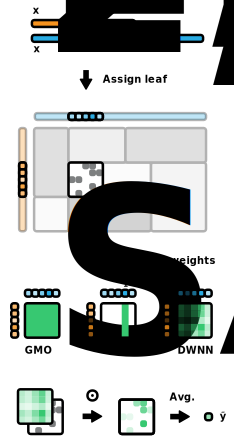
\includegraphics[width=.7\textwidth]{procedure}
%     \caption{Depiction of the inference procedure of a bipartite decision tree, visualy comparing GMO, GMOsa and the DWNN strategies for determining the final output value from the leaf partition. [mention that leaves can be discontiguous, but this is not represented]}
%     \label{fig:procedure}
% \end{figure}
% 
% The proposed approach (\autoref{sec:bipartite-model-trees}) places itself as a middle ground between the two extremes. We still utilize all the annotations in the leaf, while also still prioritizing similar instances when generating the final prediction. Therefore, we offer a more flexible framework to fine-tune biclustering decision trees along the bias-variance spectrum.
% 
% [our work for DWNN]
% 
% [dwnn allow us to use a similar idea to konstantino's also for TT]
% 
% [add a more tangible example in which the original PBCT inference would not be ideal]



\section{Experimental Setup}
\label{sec:experimental setup}

In this section, we describe the validation procedure and materials used in this work. First, we present the evaluation protocol utilized, followed by datasets and comparison methods. We publicly disclose all the code and data necessary to reproduce our results (see \autoref{sec:availability}).


\subsection{Validation procedure of bipartite learning problems}
\label{sec:bipartite validation}

% mention semi-inductiveness
% 

%There are two ways of splitting bipartite datasets into a training set (also called the learning set) and testing sets to validate machine learning models: \emph{instance-wise} and \emph{dyad-wise} splits.
There are two ways of splitting bipartite datasets into learning\footnote{Most commonly called the \emph{training} set. We call it the \emph{learning} set in order to represent it with an L and simplify the acronyms, as previously done by \cite{schrynemackers_protocols_2013,pliakos_global_2018}.} and test sets to validate machine learning models: \emph{instance-wise} and \emph{dyad-wise} splits.
We analyse results for all split types by first performing an instance-wise split in each dimension, resulting in four partitions of the dataset, and then performing a dyad-wise split on the partition with learning rows and learning columns.
This results in the four test sets defined below and illustrated in \autoref{fig:train test split}.
%Although scores were calculated for each of them,
%the inductive setting is our main focus, as described in \autoref{sec:bipartite learning}.
%Further, we explain the splitting process in more detail, and an illustration is provided by \autoref{fig:train test split}.
%
\begin{itemize}
    \item \textbf{Learning set (LD):}
    $(X_\text{1, learning},\;X_\text{2, learning}, \;Y_\text{learning dyads})$
    \item \textbf{Transductive test set (TD):}
    $(X_\text{1, learning},\;X_\text{2, learning}, \;Y_\text{test dyads})$
    \item \textbf{Semi-inductive test sets:}
    \begin{itemize}
        \item \textbf{Column-inductive test set (LT):}
            $
                (X_\text{1, learning},
                \;X_\text{2, test},
                \;Y_\text{learning rows, test columns})
            $
        \item \textbf{Row-inductive test set (TL):}
            $
                (X_\text{1, test},
                \;X_\text{2, learning},
                \;Y_\text{test rows, learning columns})
            $
    \end{itemize}
    \item \textbf{Inductive test set (TT):}
    $(
        X_\text{1, test},
        \;X_\text{2, test},
        \;Y_\text{test rows, test columns}
    )$
\end{itemize}

\begin{figure}[bth]
    \centering
    \def\svgscale{.3}
    \input{figures/illustrations/split.pdf_tex}
    \caption{Diagram of the training and test sets in the bipartite context (see \autoref{sec:bipartite validation}).}
    \label{fig:train test split}
\end{figure}
 
%There are two ways of splitting bipartite datasets into learning (or training) and testing sets to validate machine learning models. We call them \emph{instance-wise} and \emph{dyad-wise} splits.

%Instance-wise splits partition the instances and corresponding outputs separately for each dimension: $(X_1,\; Y)$ into $(X_\text{1, learning}, Y_\text{learning rows})$ and $(X_\text{1, test},\; Y_\text{test rows})$, or the same for $X_2$. 
%Dyad-wise splits act on the dyads set $D$ directly, partitioning it into $(D_\text{learning},\; Y_\text{learning dyads})$ and $(D_\text{test}, \; Y_\text{test dyads})$.
%%(in our case, $Y_\text{learning rows, learning columns} = Y_\text{learning dyads} \cup Y_\text{testing dyads}$).
%%
%Notice that there is no guarantee that an instance $\x_1$ in $D_\text{test}$ would not also be present in $D_\text{learning}$.
%%Notice that there is no guarantee that an instance $\x_1 \in \mathcal{X}_1$ or $\x_2 \in \mathcal{X}_2$ in $D_\text{test}$ would not also be present in $D_\text{learning}$.
%%Notice that there is no guarantee that an instance $\x \in \mathcal{X}_1 \cup \mathcal{X}_2$ in $D_\text{test}$ would not also be present in $D_\text{learning}$.
%Therefore, we must work with the assumption that $D_\text{test}$ can be constructed from $D_\text{learning}$, which effectively means that only the set of known outputs $Y$ is split into learning and test sets: $(X_1,\; X_2,\; Y)$ into $(X_1,\; X_2,\; Y_\text{learning dyads})$ and $(X_1,\; X_2,\; Y_\text{test dyads})$.
%In other words,
Dyad-wise splits intrinsically imply a \emph{transductive}~\cite{chapelle_semi-supervised_2006,lu_link_2011,zhou_semi-supervised_2021} learning setting.
%
Therefore, although common in the literature, dyad-wise splitting fails to evaluate the ability of a model to generalize to unseen instances (called \emph{inductiveness}), as pointed out by \cite{park_flaws_2012,schrynemackers_protocols_2013,pahikkala_toward_2015}.
Various names for this partitioning procedure and test sets have been proposed in the literature~\cite{park_flaws_2012,schrynemackers_protocols_2013,pahikkala_toward_2015,liu_neighborhood_2016,pliakos_global_2018}. We opt for the concise two-letter acronyms above.

%Although each split type could be analysed separately~\cite{pliakos_global_2018}, we choose to analyse them together
%We analyse results for all split types by first performing row- and column-wise splits, resulting in four partitions of the dataset, and then performing a dyad-wise split on the partition with learning rows and learning columns.

%In the case of positive-unlabeled learning, the positive annotations represent all information available, and the dyad-wise split may only consider the set $Y_+$ of positive dyads ($y=1$), while the negative dyads $Y_-$ ($y=0$) are used for both training and testing: $D$ is divided between $D_\text{+, learning} \cup D_-$ and $D_\text{+, testing}$.


% %
% %Accordingly, we call the training set the \emph{LL set}.
% %LL, TL, LT, and TT were already presented with similar names in previous work~\cite{schrynemackers2015classifying,pliakos2018global,pliakos2020drugtarget}. %TODO other previous paper before schrynemackers2015
% %The authors call them $L_r \times L_c$, $T_r \times L_c$, and so on.
% %\cite{pahikkala2015more,ezzat2019computational,liu2016neighborhood} denotes LL-U, LT, TL and TT as S1, S2, S3 and S4, respectively.
% %\cite{liu2016neighborhood} uses a similar notation, but uses S1 to designate LL-M instead of LL-U. % TODO CHECK
% %%
% %The LL-U test set is most frequently used when building SGSO models~\cite{pahikkala2015more}.
% %%\cite{huang2020moltrans} also reports TL and LT scores.
% %Using LL-M is more common for matrix factorization methods~\cite{liu2016neighborhood,hao2017predicting,li2019dnilmflda}.



\subsection{Bipartite Cross-Validation}
\label{sec:cv}

Two-dimensional splitting was performed for cross-validation, similarly to \cite{schrynemackers_classifying_2015,pliakos_drug-target_2020}. Each of the two instance sets was split into $k$ folds, using stratification to encourage consistent fold densities. The row fold-column fold combinations yield $k^2$ TT test sets (see \autoref{sec:bipartite validation}). The corresponding semi-inductive test sets were also collected for each TT set, and the training set and transductive test set are then generated.
The value of $k$ was adjusted for each learning task, using more folds for smaller datasets (\autoref{tab:datasets}).
%\autoref{fig:cv} illustrates this procedure.

%To generate the transductive test set, we randomly sampled a percentage $p$ of the positive annotations, splitting the set of positive annotations $Y_+$ into $Y_\text{+, learning}$ and $Y_\text{+, test}$. These annotations were masked (replaced by $0$s) to generate the matrix representation of $Y_\text{learning dyads}$. For transductive evaluation, 

In our case of positive-unlabeled learning~\cite{bekker2020learning}, the set $Y$ consists only of positive annotations. A percentage of these annotations was then held out for generating the transductive test set $Y_\text{test dyads}$. In the matrix representation of $Y_\text{learning dyads}$, this means masking the positive annotations by turning them into zeros. We therefore refer to this quantity as the \emph{positives masking percentage} (PMP).
%the missing and held out annotations are represented as $0$s.
All the missing annotations in $Y$ (zeros that were not generated by the masking) were used as negative annotations for evaluation in the transductive setting. We explored four values for PMP: $0\%$, $25\%$, $50\%$, and $75\%$.
%In the matrix representation of 
%In the case of positive-unlabeled learning, the positive annotations represent all information available, and the dyad-wise split may only consider the set $Y_+$ of positive dyads ($y=1$), while the negative dyads $Y_-$ ($y=0$) are used for both training and testing: $D$ is divided between $D_\text{+, learning} \cup D_-$ and $D_\text{+, testing}$.

\subsection{Evaluation measures and statistical tests}
\label{sec:evaluation}

In a similar fashion to \cite{schrynemackers_protocols_2013,pliakos_global_2018,pliakos_drug-target_2020,liu_drug-target_2022}, we have employed the area under the precision and recall curve (AUPRC) and the area under the ROC curve (AUROC) to measure the performance.
%The AUPR is defined as the area under the curve generated using Precision (\autoref{eq:metrics}) in the x-axis and Recall (\autoref{eq:metrics}) in the y-axis, considering multiple classification thresholds. Similarly, the ROC curve is defined as the recall (true positive rate, \autoref{eq:metrics}) against the false positive rate (FPR, \autoref{eq:metrics}).    
%
%\begin{align}
%    % \label{eq:precision}
%    \text{Precision} = \frac{TP}{TP + FP}
%    % \label{eq:recall}
%    && \text{Recall} = \frac{TP}{TP + FN}
%    % \label{eq:fpr}
%    % && \text{FalsePositiveRate} = \frac{FP}{FP + FN}
%    && \text{FPR} = \frac{FP}{FP + FN}
%    \label{eq:metrics}
%\end{align}
%
% \begin{equation}
%     \label{eq:precision}
%     \text{Precision} = \frac{TP}{TP + FP}
% \end{equation}
% 
% \begin{equation}
%     \label{eq:recall}
%     \text{Recall} = \frac{TP}{TP + FN}
% \end{equation}
% 
% \begin{equation}
%     \label{eq:fpr}
%     \text{FalsePositiveRate} = \frac{FP}{FP + FN}
% \end{equation}
%
Moreover, we have employed the Friedman test, followed by the post-hoc Nemenyi test, as suggested in \cite{demsar_statistical_2006}. Graphically, the results are displayed in a critical difference diagram where methods placed in lower ranks are associated to better performance. Further, methods connected by a horizontal bar are not statistically significantly different.


%Furthermore, we have performed X-FOLD cross validation. It is worth noting that the cross-validation procedure in interaction prediction differs significantly from other machine learning tasks. As illustrated in Figure X, a dataset is divided into 4 partitions:

%\begin{itemize}
 %   \item TT: The train partition which contains X1, X2 and their respective interactions, Y;
  %  \item LT: A test partition where X2 contains unseen instances, but X1 was present in TT;
   % \item LT: A test partition where X1 contains unseen instances, but X2 was present in TT; 
    %\item LL: A test partition where both X1 and X2 were not present in the train partition (TT); 
    
%\end{itemize}


%We report our results using ....... explain diagram that we have


\subsection{Datasets}
\label{sec:datasets}

\autoref{tab:datasets} describes the datasets used in this work. As can be seen, we have employed a total of 15 datasets from several biological domains, including drug-target, RNA-disease and RNA-RNA interactions. In this case, all features correspond to similarities measured on the instances of an input space of the problem. For instance, the features of dataset DPI-E associated to $X_1$ (drugs) correspond to the similarities among instances from $X_1$ (drugs). Its counterpart, $X_2$, contains similarities among the instances from $X_2$, enzymes.

\begin{table}[ht]
\tiny
% \begin{tabular}{llll}
% \toprule
% Dataset        & Domain                    & Dimensionality    & Density \\ \midrule
% DPI-E          & Drug-enzyme               & 664 $\times$ 445  & 1.0\%   \\
% DPI-G          & Drug-GPCR                 & 95 $\times$ 223   & 3.0\%   \\
% DPI-I          & Drug-ion channel          & 204 $\times$ 210  & 3.5\%   \\
% DPI-N          & Drug-nuclear receptor     & 26 $\times$ 54    & 6.4\%   \\
% ERN            & Gene-transcription factor & 1164 $\times$ 154 & 1.8\%   \\
% SRN            & Gene-transcription factor & 1821 $\times$ 113 & 1.9\%   \\
% DAVIS          & Inhibitor-kinase          & 68 $\times$ 442   & 5\%     \\
% KIBA           & Inhibitor-kinase          & 2119 $\times$229  & 19.7\%  \\
% NPInter        & lncRNA-protein            & 586 $\times$ 446  & 18.1\%  \\
% mirTarBase     & miRNA-mRNA                & 1873 $\times$ 415 & 7.0\%   \\ 
% Lnc2Cancer     & lncRNA-cancer             & 367 $ \times 106$  & 0.1\%   \\
% LncRNA-disease & lncRNA-disease            & 156 $ \times 241$  & 0.1\%   \\
% LncRNA-miRNA   & lncRNA-miRNA              & 44 $ \times 218$   & 0.1\%   \\
% MiRNA-disease  & miRNA-disease             & 462 $ \times 252$  & 0.1\%   \\
% TE-piRNA       & TE-piRNA                  & 60 $ \times 93$    & 0.04\% \\ \bottomrule
% \end{tabular}
\begin{tabular}{llllrrl}
\toprule
Name & Domain & Dimensionality & Folds & Dyads & Positives & Density \\
\midrule
DPI-N & Drug-Nuclear receptor & $26 \times 54$ & $4 \times 4$ & 1404 & 90 & 6.41\% \\
TE-Pirna & Transposable element-piRNA & $60 \times 93$ & $4 \times 4$ & 5580 & 219 & 3.92\% \\
LncRNA-miRNA & LncRNA-miRNA & $44 \times 218$ & $3 \times 3$ & 9592 & 983 & 10.2\% \\
DPI-G & Drug-GPCR & $95 \times 223$ & $3 \times 3$ & 21185 & 635 & 3\% \\
Davis & Inhibitor-Kinase & $68 \times 442$ & $3 \times 3$ & 30056 & 1506 & 5.01\% \\
LncRNA-Disease & LncRNA-Disease & $156 \times 241$ & $3 \times 3$ & 37596 & 2485 & 6.61\% \\
LncRNA-Cancer & LncRNA-Cancer & $367 \times 106$ & $3 \times 3$ & 38902 & 2836 & 7.29\% \\
DPI-I & Drug-Ion channel & $204 \times 210$ & $2 \times 2$ & 42840 & 1476 & 3.45\% \\
MiRNA-Disease & MiRNA-Disease & $462 \times 252$ & $2 \times 2$ & 116424 & 13448 & 11.6\% \\
ERN & Gene-Transcription factor & $1164 \times 154$ & $2 \times 2$ & 179256 & 3293 & 1.84\% \\
SRN & Gene-Transcription factor & $1821 \times 113$ & $2 \times 2$ & 205773 & 3663 & 1.78\% \\
NPInter & LncRNA-Protein & $586 \times 446$ & $2 \times 2$ & 261356 & 47353 & 18.1\% \\
DPI-E & Drug-Enzyme & $664 \times 445$ & $2 \times 2$ & 295480 & 2926 & 0.99\% \\
KIBA & Inhibitor-Kinase & $2111 \times 229$ & $2 \times 2$ & 483419 & 95443 & 19.7\% \\
miRTarBase & MiRNA-Target gene & $1873 \times 415$ & $2 \times 2$ & 777295 & 54913 & 7.06\% \\
\bottomrule
\end{tabular}
\caption{Summary of the datasets used in this study. }
\label{tab:datasets}
\end{table}

DPI-N, DPI-G, DPI-I, DPI-E, SRN, ERN, Davis and KIBA are widely employed in the literature \cite{schrynemackers_classifying_2015,pliakos_network_2019, pliakos_integrating_2019, pliakos_drug-target_2020, ilidio_fast_2024, alves_semi-supervised_2023}. We have preprocessed NPInter and mirTarBase in our preliminary work~\cite{ilidio_fast_2024}. We have also collected five more datasets, TE-Pirna, LncRNA-miRNA, lncRNA-disease, lncRNA-cancer, and miRNA-disease, which, to the best of our knowledge, have never been used as benchmarks for interaction prediction in general.
%
For these last seven datasets, nucletide similarities were calculated using the normalized Smith-Waterman score. For the diseases, we used the similarity proposed by \citet{wang2007new}, since it is the most used one \cite{cheng2019computational}. The weight was set to 0.5.
%
Lnc2Cancer contains lncRNA-cancer interactions \cite{gao2021lnc2cancer}\footnote{http://bio-bigdata.hrbmu.edu.cn/lnc2cancer/}.
%To construct this dataset, we calculated similarities among the lncRNAs and the types of cancers. For the diseases, we used the similarity proposed by \citet{wang2007new}, since it is the most used one \cite{cheng2019computational}. The weight was set to 0.5. %The similarities among the lnc-RNAs were calculated using the normalized Smith-Waterman score.
%
The datasets LncRNA-disease, LncRNA-miRNA and miRNA-disease were made available in \cite{sheng2023data}, where the authors collected data from several repositories.
%The RNA similarities were calculated using the method proposed in \cite{chen2015constructing}. The miRNA similarities were calculated \cite{wang2010inferring}. Lastly, the disease similarity was once again measured using the method proposed by Wang \cite{wang2007new}
%The disease similarity was once again measured using the method proposed by Wang \cite{wang2007new}.
%
TE-piRNA contains interaction between transposable elements (TEs) and piwi-RNAs (piRNAs), and was collected by~\cite{dos2024transposable}.
%and both of them had their similarities calculated from the normalized Smith-Waterman, as aforementioned.
%The authors extracted Pse-in-One features from both TEs, which were used as input to the normalized Smith-Waterman score, thus generating similarities. 

% \begin{table}
% \begin{tabular}{lll}
% \toprule
% Name & Shape & Density \\
% \midrule
% dpin & $26 \times 54$ & 0.064 \\
% dpig & $95 \times 223$ & 0.03 \\
% dpii & $204 \times 210$ & 0.034 \\
% dpie & $664 \times 445$ & 0.0099 \\
% srn & $1821 \times 113$ & 0.018 \\
% ern & $1164 \times 154$ & 0.018 \\
% davis & $68 \times 442$ & 0.05 \\
% kiba & $2111 \times 229$ & 0.2 \\
% mirtarbase & $1873 \times 415$ & 0.071 \\
% npinter & $586 \times 446$ & 0.18 \\
% lncrnacancer & $367 \times 106$ & 0.073 \\
% lncrnadisease & $156 \times 241$ & 0.066 \\
% lncrnamirna & $44 \times 218$ & 0.1 \\
% mirnadisease & $462 \times 252$ & 0.12 \\
% tepirna & $60 \times 93$ & 0.039 \\
% \bottomrule
% \end{tabular}
% \end{table}


 %lncrna-cancer, lncrna-disease, lncrna-mirna, mirna-disease e te-pirna


\subsection{Comparison methods}
\label{sec:baselines}

In this section we present a list of the comparison methods used in this work. We provide more details about them in \autoref{sec:baselines details}.
Regarding hyperparameter tuning, a nested 2 by 2 cross-validation procedure was utilized, using AUPRC to select the best hyperparameter combination for each outer fold.
The specific hyperparameter sets considered for each method are also presented in \autoref{sec:baselines details}. Finally, refer to \autoref{sec:data-based} for descriptions of the global single output (GSO) and local multi-output (LMO) approaches.

\begin{itemize}
%\item Logistic: baseline logistic regression built using the GSO approach; 
\item MLP: baseline multi-layer perceptron built using the GSO approach. Random undersampling of negative annotations was used, resulting in balanced training datasets;

\item RLS-avg: baseline regularized least squares built using the LMO approach and a Gaussian network kernel~\cite{van_laarhoven_gaussian_2011};

\item RLS-Kron: Regularized least squares using the Kronecker product kernel~\cite{van_laarhoven_gaussian_nodate}, as explained in \autoref{sec:rlskron leaf}. It also uses a Gaussian network kernel~\cite{van_laarhoven_gaussian_2011};

\item BLMNII: a method built using the LMO approach, which uses a weighted-neighbors technique for the primary estimators and kernel ridge regression models as secondary estimators~\cite{mei2013drug}. It as well uses a Gaussian network kernel~\cite{van_laarhoven_gaussian_2011,mei2013drug};

\item NRLMF: Neighborhood-Regularized Logistic Matrix Factorization~\cite{liu_neighborhood_2016,liu_lpi-nrlmf_2017,liu_predicting_2020}, adapts matrix factorization to be able to perform inductive inference;

\item BICTR: The most recent PBCT-based method~\cite{pliakos_drug-target_2020}. It first reconstructs the output space using NRLMF and then builds an ensemble of predictive bi-clustering trees;

\item WkNNIR: Also proposed for inductive drug-target interaction prediction, WkNNIR uses ensembles of weighted nearest neighbors and interaction recovery, and was shown to surpass BICTR~\cite{liu_drug-target_2022};

\item Oxytrees[Deep, YR]: A variant of our method (\autoref{sec:oxytrees}) evalutated as a direct comparison to BICTR. It also uses NRLMF interaction matrix reconstruction (YR), and then builds an ensemble of Oxytrees, inducing the trees until leaf homogeneity instead of using leaf models;

\item Oxytrees[Logistic]: A baseline variant of our proposed method (\autoref{sec:oxytrees}) using a logistic regression trained using the GSO approach as the leaf model;

\item Oxytrees[RLS-Kron]: An ensemble of our main proposed method,  Oxytrees, using RLS-Kron as the leaf model (\autoref{sec:oxytrees});

\end{itemize}



% recover positives
% internal nrlmf validation
% feature subsampling

% [discuss network kernel of rls-kron and blmnii]


\section{Results and discussion}
\label{sec:results}
\FloatBarrier

In this section, we initially present results regarding the predictive performance of our Oxytrees in comparison to previous approaches. Next, we perform an ablation study to assess the effects of adding a leaf model and a matrix completion pre-training step to biclustering trees. Lastly, we analyse the computational complexity of our algorithms in comparison to the previous biclustering tree method.


\subsection{Comparing Oxytrees against previous proposals}
\label{sec:literature comparison}

%[auroc should be a more stable metric compared to auprc given the PU setting]

%[auprc should be preferable for early retrieval]

%[fully grown trees are better for auprc because they can model the underlying missingness mechanism]

%Oxytrees[RLS-Kron] is better than RLS-Kron alone

In this section, we compare three versions of our proposed models with several baselines from the literature, using the datasets described in \autoref{sec:datasets}. The results are presented by \autoref{fig:literature inductive}.
%
\begin{figure}[tbh]
    \centering
    \begin{subfigure}{\textwidth}
        \includegraphics[width=.49\textwidth]{results/literature_methods/TT/all_datasets/critical_difference_diagrams/AUROC (Inductive).pdf}
        \hfill
        \includegraphics[width=.49\textwidth]{results/literature_methods/TT/all_datasets/critical_difference_diagrams/AUPRC (Inductive).pdf}
        \caption{Positives masking percentage = 0\%}
    \end{subfigure}
    
    \begin{subfigure}{\textwidth}
        \includegraphics[width=.49\textwidth]{results/literature_methods/TT_25/all_datasets/critical_difference_diagrams/AUROC (Inductive).pdf}
        \hfill
        \includegraphics[width=.49\textwidth]{results/literature_methods/TT_25/all_datasets/critical_difference_diagrams/AUPRC (Inductive).pdf}
        \caption{Positives masking percentage = 25\%}
    \end{subfigure}
    
    \begin{subfigure}{\textwidth}
        \includegraphics[width=.49\textwidth]{results/literature_methods/TT_50/all_datasets/critical_difference_diagrams/AUROC (Inductive).pdf}
        \hfill
        \includegraphics[width=.49\textwidth]{results/literature_methods/TT_50/all_datasets/critical_difference_diagrams/AUPRC (Inductive).pdf}
        \caption{Positives masking percentage = 50\%}
    \end{subfigure}
    
    \begin{subfigure}{\textwidth}
        \includegraphics[width=.49\textwidth]{results/literature_methods/TT_75/all_datasets/critical_difference_diagrams/AUROC (Inductive).pdf}
        \hfill
        \includegraphics[width=.49\textwidth]{results/literature_methods/TT_75/all_datasets/critical_difference_diagrams/AUPRC (Inductive).pdf}
        \caption{Positives masking percentage = 75\%}
    \end{subfigure}   

    \caption{Comparisons of AUROC (on the left) and AUPR (on the right) of the proposed Oxytrees against previous methods for bipartite learning. The inductive setting is analysed, across four different values for the positives dropout percent (see \autoref{sec:bipartite validation}).
    }
    \label{fig:literature inductive}
\end{figure}
%
Oxytrees[RLS-Kron] had the best average ranking for all positives masking percentages analysed.
Remarkably, Oxytrees[RLS-Kron] trains expressively faster than BICTR, as thoroughly measured in \autoref{sec:empirical complexity}.
Average values for AUROC and AUPRC in each dataset are presented by \autoref{tab:auroc} and \autoref{tab:auprc}, respectively.

We also see that Oxytrees perform consistently better than RLS-Kron alone, strongly indicating that the tree structure does provide substantial advantages to the algorithm. It suggests that RLS-Kron is better suited to model the smaller groups of instances in each leaf, rather than the task in its entirety. This is similar in essence to how a linear function can often locally approximate another function with more complicated behavior.
%
Although not the focus of this study, \autoref{fig:literature semi-inductive} presents results for the semi-inductive setting. Oxytrees[RLS-Kron] were again the best model for all settings in terms of AUPRC. In terms of AUROC, Oxytrees[RLS-Kron], Oxytrees[Deep, YR] and BICTR had close results.
%
For the transductive setting with 0\% PMP (\autoref{fig:literature transductive}), NRLMF, BICTR and Oxytrees[Deep, YR] had very close scores, pointing that NRLMF alone is sufficient in this scenario. When more interactions are masked (\autoref{fig:literature transductive}), the forests apparently result in slight improvements, but further experiments are needed for confirmation.
%
These results clearly highlight the potential of Oxytrees for bipartite learning: Oxytrees[RLS-Kron] consistently displayed the best performance despite often running an order of magnitude faster than BICTR, its strongest competitor in terms of AUROC.

% 1 - Difference in performance between models at the leaf: KronRLS vs Logistic
Comparing the two different leaf models in all settings, we observe consistent superiority of Oxytrees[RLS-Kron] against Oxytrees[Logistic]. A crucial difference between the two models is that RLS-Kron uses all combinations $\phi_1^i\phi_2^j$ between elements of the feature vectors $\phi_1$ and $\phi_2$ in each domain, while the logistic regressor uses $\phi_1$ concatenated with $\phi_2$. We argue that the superior performance of RLS-Kron is due to this extra complexity: the larger number of input features seems to still be necessary to capture the behavior of our data.

% 2 - Difference between NLRMF + Oxytrees (Deep) and BICTR performance wise
Comparing Oxytrees[Deep, YR] against BICTR, we notice that the Oxytrees perform slightly better in almost all scenarios, and remarkably close otherwise. This is expected, since the only fundamental difference between the models is their impurity function (\autoref{sec:oxytrees impurity}). However, the expressive computational advantage of Oxytrees (\autoref{sec:oxytrees training} and \autoref{sec:empirical complexity}) indicates Oxytrees as the best option even for scenarios where BICTR was dominant.

%  6- Discuss numbers from the tables. Say that despite our method achieving better results and expanding the state-of-the-art, this problem is still very challenging since the numbers are overall still low
Considering the values for AUPRC and AUROC for each dataset (Tab. \ref{tab:auprc} and \ref{tab:auroc}), we notice very different results for each task, suggesting that the choice of predictive algorithm to use must take into consideration the specific scenario of the learning problem. Furthermore, the scores in the inductive (Tab. \ref{tab:auprc} and \ref{tab:auroc}) and semi-inductive (Tab. \ref{tab:auprc lt}, \ref{tab:auroc lt}, \ref{tab:auprc tl} and \ref{tab:auroc tl}) settings are considerably lower compared to the transductive setting (Tab. \ref{tab:auprc transductive} and \ref{tab:auroc transductive}), which highlights the general difficulty of considering new instances.

%Besides the computational advantages of Oxytrees, the main distinction between the two methods is the impurity function they use.
%%Oxytrees prioritize label columns that are correlated to select splits, while BICTR treats each label column independently (see \autoref{sec:oxytrees impurity}). We hypothesize that this characteristic of Oxytrees 
% BICTR tends to group either row \emph{or} column instances with similar labels when selecting splits, while Oxytrees tend to group \emph{dyads} with similar labels (see \autoref{sec:oxytrees impurity}). %, that is, both rows \emph{and} columns are considered together (see \autoref{sec:oxytrees impurity}).
% We hypothesize that exploring both domains at the same time is especially useful when more positive annotations are missing: for Oxytrees, if a negative dyad is in a tree node with many positive dyads, it is likely that the negative dyad is a wrongly annotated positive, since all dyads in the same node are likely to have the same label. The same is not true for BICTR and PBCTs: a truly negative dyad can be placed in a node with very similar row instances, for example, but since the column instances may considerably differ, we expect the dyads in the node to still have very different true labels. Therefore, the clustering performed by Oxytrees is more likely to reflect the true labels of the dyads and thus to be more resistant to missing annotations.
%
% 4 - Differences between the different percentages of masking 
%In accordance with this hypothesis, BICTR seems to perform comparatively worse overall as missing positives increase, especially in terms of AUROC.

% 5 - Relate the topics above with AUPRC vs AUROC
%This pattern is less clear for AUPRC, which is explained by the fact that AUPRC prioritizes the test dyads with the highest predicted probabilities~\cite{saito_precision-recall_2015}. Therefore, AUPRC would be already high if a model can correctly select a small set of dyads that are very likely to be positive, and positive dyads with low predicted probability are overlooked.
 
% 3 - Short sentence about performance of the baselines. Local vs Global. Kron is still quite strong bla bla, local methods are not doing that great. NRLMF by itself is not great either, mb that has an effect on the reconstruction...... 
Regarding the baselines other than BICTR, RLS-avg and RLS-Kron show the overall best performance (\autoref{fig:literature inductive}), followed by RLS-avg. Their performance was only worse than Oxytrees[RLS-Kron] for AUPRC, and worse than all tree-based models for AUROC.
%, suggesting that linear models could be a reasonable option if computational resources are limited.
On the other hand, NRLMF was one of the worst performers in the inductive setting compared to the other models. This shows that the original promising results of NRLMF in the transductive setting (found by \citet{liu_neighborhood_2016,liu_lpi-nrlmf_2017,liu_predicting_2020} and reproduced by us in \autoref{fig:literature transductive}) do not translate into the inductive setting. This also motivates the previously proposed combination of NRLMF and biclustering forests~\cite{pliakos_drug-target_2020}, restricting NRLMF to the transductive step of matrix completion and delegating the inductive modeling to the forest.
Furthermore, WkNNIR was not able to outperform BICTR in our experiments with 15 datasets, contrary to what was observed for drug-target interaction prediction~\cite{liu_drug-target_2022}.

% 4 - Differences between the different percentages of masking 
% oxytrees[kron] are better than other forests
% mlp has a jump in performance, probably due to architechture change




%% 5 - Relate the topics above with AUPRC vs AUROC
%We also notice that the linear models RLS-avg and RLS-Kron seem to be favored by AUPRC in comparison fo AUROC. This could be a result of AUPRC being chosen as the objective for hyperparameter optimization (\autoref{sec:baselines}). That being true, it would imply that using the Gaussian network kernel improves performance of these models, even in the inductive scenario. On a more fundamental level, AUPRC is more dependent on the highest predicted probabilities, and less sensitive to how the model performs in terms of the lowest predicted probabilities~\cite{schrynemackers_protocols_2013,saito_precision-recall_2015}. Therefore, the diverging results between AUPRC and AUROC can also be explained by the most likely interactions behaving linearly while less likely interactions having more complex behavior.
%%
%In any case, the linear models are still outperformed by Oxytrees[RLS-Kron], suggesting that Oxytrees can leverage this property of linear models while also encompassing less likely interactions.
%%
% An illustration of this idea is presented by \autoref{fig:}.
%%We refer to \cite{schrynemackers_protocols_2013} for a more in-depth discussion on the differences between AUROC and AUPRC in the context of interaction prediction.
%In conclusion, RLS-avg or RLS-Kron can be valuable alternatives for early-retrieval if computational resources are limited, while Oxytrees should be preferred in general if enough resources are available. An example of early-retrieval scenario is selecting just a handful of very likely drug-protein interactions to be experimentally validated.



%We first analyze the inductive case where the dyads being tested are completely new to the model, making it more challenging than its semi-inductive counterpart.    

%As can be seen in Figure X, in the inductive analysis, our proposed method, Oxytrees using DWN leads to superior results in most of the cases, specially regarding AUROC. More specifically, we see that Oxytrees(DWN) using NLRMF ranks higher in all evaluated cases, with statistical significance when 50\% and 75\% of the positive annotations are masked. That is, in the more extreme cases, where very few confirmed interactions are available, NRLMF + Oxytrees(DWN) leads to better performance. However, when considering the supervised case (0\%) and 25\% of masking, we observed no statistical significant difference between BiCTR and Oxytrees(RLS-Kron) 

%Regarding AUPRC, as shown in the lower part of Figure X, we noticed a less consistent pattern where Oxytrees(RLS-Kron) without NLRMF yielded better results among our variants, nonetheless, in general, BICTR and NRLMF + BGSO also produced competitive results. In this case, no statistical difference was observed among these three methods. Surprisingly, NRLMF + Oxytrees(DWN) was not competitive in most of the cases, except on the 75\% experiments. 


%Furthermore, we also notice that all baselines, DWN, MLP, NLRMF, BLMNII(RLS), LMO(RLS), performed very poorly, being consistently statistically outperformed by the other methods. RLS-Kron managed to statistically outperform the baselines in the majority of the cases, nonetheless it is still underwhelming when compared to  BICTR and variants of the Oxytrees. This highlights the potential of model trees, as combining NRLMF + BGSO with models such as, DWN or RLS-Kron, statistically improves the performance.       



% Paragraph about reasoning between difference in performance between AUPRC and AUROC
 

%Further, as aforementioned, interaction prediction is assumed to be a case of positive-unlabeled learning, thus reconstructing the output space is a logical step to account for unconfirmed negative annotations. Hence, it could be expected that the performance of any model would improve, as more possible positive annotations are made available. However, that is not always the case. As the benefits of NRLMF in the supervised case (0/%) are rather minimal. This could be partially credited to the quality of the reconstruction, as NLRMF, despite being originally proposed in this context, is not a competitive method on its own. 

%@PEDRO OTHER INFO THAT YOU WANT TO ADD


%s
%SEMI-INDUCTIVE,

%In the semi-inductive analysis, an unexpected behavior is noticed as NRLMF + Oxytrees (DWN) nor Oxytrees (RLS-Kron) do not lead superior results in neither of the evaluation metrics. When considering AUROC (Figure Z, upper part), we see that NRLMF + BGSO, thus Oxytrees using the average prediction at the leaves, systematically ranks first among all methods. Similarly to the inductive case, we noticed a more prominent difference when 50\% or 75\% of the annotations are masked. In these cases, NRLMF + BGSO statistically outperforms BICTR. Similarly (Figure Z, lower part), in terms of AUPRC, RLS-Kron is always ranked in the first position, nonetheless BICTR and NRLMF + BGSO are statistically equivalent. Once again, baselines failed to achieve desirable performance.  

%Considering that part of the test instances are used to construct both decision trees and its models at the leaves, as seen in Section X, the lower performance provided by the model trees is rather surprising. Given that predicting the average at leaves is mostly superior than using a model, we may suppose that the leaf models are overfitting to the interactions available in the training dataset, and thus failing to genralize to other instances.

%The fact that RLS-Kron, a relatively older method, very frequently outranks other competitors may emphaize the idea of overfitting. Despite DOING SOMETHING FODA, RLS-Kron is still a linear model which DOES STHM. Thus, the combination of a decision tree, a non-linear model, with a linear model should, in principle, should have easily surpassed RLS-Kron.

%@PEDRO MORE STUFF TO TALK ABOUT? 




\subsection{Ablation study}
\label{sec:ablation}

%To further validate our method, we perform an ablation study to analyze its performance. We consider the following hypotheses:
In this section, we investigate two hypotheses regarding the components of Oxytrees:

%In fact, a main rationale behind model trees is to combine a simple high-bias model (such as linear regression) with the high-variance and low-bias decision trees, balancing their respective strengths and weaknesses. Although simple models are often insufficient to represent the data as a whole, they often provide good local approximations to the learning task. Using a decision tree allows these models to be applied separately to specific regions of the feature space, in a similar fashion to how a nonlinear function can often be locally approximated by a linear one.

% TODO: Another benefit would be in terms of computational complexity...

%However, two trivial explanations must be ruled out for the hypothesized benefits to hold and for the proposed approach to be justifiable:
%
\begin{enumerate}
    %\item \textbf{The leaf model is doing all the work:} the simple model is already able to capture the underlying patterns in the data, and the tree partitioning is not adding any value to the model.
    %\item \textbf{Large leaves are enough:} setting the leaf size to be large enough would already provide the same benefits as the proposed approach. % This corresponds to setting the leaf model to the simplest possible estimator: the label average.
    \item \textbf{Large leaves could be enough:} The larger leaves of Oxytrees could be the main factor behind its superiority, and the specific leaf-model would play a minor role;
    \item \textbf{Matrix completion could aid Oxytrees:} Oxytrees could perform better if trained on reconstructed versions of the interaction matrix, generated with matrix factorization in a transductive manner. This was shown to be true for PBCT ensembles using Neighborhood-Regularized Logistic Matrix Factorization (NRLMF)~\cite{pliakos_drug-target_2020}, although only in a limited set of drug-target interaction datasets.
    % \item \textbf{The specific weights are irrelevant:} the distance-based weighting procedure is not adding any value to the model, and the same results could be achieved by using random weights in the leaves. [this is hard to explain, I think it has some reason but I still have to think it through]
\end{enumerate}

For that purpose, we compare ensembles of extremely randomized Oxytrees i) using and not using NRLMF for interaction matrix reconstruction (YR), as well as ii) with RLS-Kron and without it (outputting the mean of leaf labels as usual). Importantly, the leaves of all models were kept at the same size, with minimum dimensions of 5 by 5, and all features were evaluated for splits in each tree node. The four resulting variations of our algorithm are compared in terms of AUPRC across all datasets in \autoref{fig:ablation inductive auprc}.

\begin{figure}
    \begin{subfigure}{.49\textwidth}
        \centering
        %\includegraphics[height=2.5cm]{results/y_reconstruction/TT/all_datasets/critical_difference_diagrams/AUPRC (Inductive).pdf}
        \includegraphics[width=\linewidth]{results/y_reconstruction/TT/all_datasets/critical_difference_diagrams/AUPRC (Inductive).pdf}
        \caption{Positives masking percentage = 0\%}
    \end{subfigure}
    \hfill
    \begin{subfigure}{.49\textwidth}
        \centering
        %\includegraphics[height=2.5cm]{results/y_reconstruction/TT_25/all_datasets/critical_difference_diagrams/AUPRC (Inductive).pdf}
        \includegraphics[width=\linewidth]{results/y_reconstruction/TT_25/all_datasets/critical_difference_diagrams/AUPRC (Inductive).pdf}
        \caption{Positives masking percentage = 25\%}
    \end{subfigure}
    
    \begin{subfigure}{.49\textwidth}
        \centering
        %\includegraphics[height=2.5cm]{results/y_reconstruction/TT_50/all_datasets/critical_difference_diagrams/AUPRC (Inductive).pdf}
        \includegraphics[width=\linewidth]{results/y_reconstruction/TT_50/all_datasets/critical_difference_diagrams/AUPRC (Inductive).pdf}
        \caption{Positives masking percentage = 50\%}
    \end{subfigure}
    \hfill
    \begin{subfigure}{.49\textwidth}
        \centering
        %\includegraphics[height=2.5cm]{results/y_reconstruction/TT_75/all_datasets/critical_difference_diagrams/AUPRC (Inductive).pdf}
        \includegraphics[width=\linewidth]{results/y_reconstruction/TT_75/all_datasets/critical_difference_diagrams/AUPRC (Inductive).pdf}
        \caption{Positives masking percentage = 75\%}
    \end{subfigure}   

    %\caption{Performance comparison of the proposed Oxytrees with and without matrix completion. [complement]}
    \caption{AUPRC comparison in the inductive case, of Oxytrees with and without a leaf model, as well as using and not using matrix completion with NRLMF.}
    \label{fig:ablation inductive auprc}
\end{figure}

In all cases, Oxytrees using RLS-Kron performed better than those returning the mean label. Specifically, Oxytrees[RLS-Kron] significantly outperformed Oxytrees[Mean] for 0\% and 25\% positives masking. Furthermore, Oxytrees[RLS-Kron] without NRLMF had a better average rank than Oxytrees[RLS-Kron, YR] using NRLMF in the settings with 0\% and 25\% masking, but no statistical significance is observed. For 50\% and 75\%, their results are very close.
%
These results are summarized~by
%
\begin{enumerate}
    \item Using RLS-Kron as a leaf model significantly improves the average performance of biclustering single output forests, asserting the effectiveness of Model Trees for bipartite learning;
    \item Matrix reconstruction seems to not improve or even harm the performance of Oxytrees[RLS-Kron] in most cases.
    %, although further experiments are needed to statistically verify this result.
\end{enumerate}
%
%The first result implies that RLS-Kron is able to model the interactions in the leaves better than the simple label averages, maintaining potential for generalization.
%The second result could be explained by a) the predictions of NRLMF are not representative of our data; b) NRLMF is less representative than RLS-Kron and the RLS-Kron models are overfitting the predictions from NRLMF; c) the predictions of NRLMF cannot be effectively modeled by the linear relationship of RLS-Kron (the leaf models underfit the NRLMF predictions). We discard (a) by observing that NRLMF does not seem to harm the performance of Oxytrees[Mean], and also by noticing that NRLMF consistently performs better than a random baseline (for example, AUROC $>$ 0.5 in \autoref{tab:auroc}) and displays one of the best performances in the transductive case (\autoref{fig:literature transductive} and \autoref{tab:auprc transductive}). Regarding (b), RLS-Kron performs better than NRLMF when compared directly (\autoref{sec:literature comparison}), which seems to corroborate the hypothesis. However, the performance of Kron-RLS could deteriorate when applied to the small leaf partitions, and further experiments are required to investigate hypotheses (b) and (c).

%
No statistically significant results were obtained for AUROC, as shown in \autoref{fig:ablation inductive auroc}.% in \autoref{sec:additional results}.

% \subsubsection{Using similarities with neighbors is the best way of generating outputs}
% \subsubsection{Larger leaves are not enough to explain the performance improvement}

\subsection{Empirical computational complexity analysis}
\label{sec:empirical complexity}
%\subsection{Run time comparison}

In this section, we empirically assess the theoretical results presented in \autoref{sec:oxytrees training} and in \autoref{sec:batch inference} regarding the computational complexity of our algorithms. For all cases, we generate artificial training sets $X_1$, $X_2$ and $Y$ by filling three $n \times n$ matrices with uniform pseudo-random values between 0 and 1. \autoref{fig:fit complexity} compares extremely randomized versions of a single Oxytree[RLS-Kron], a single Oxytree[Deep] and a single PBCT[Deep] for multiple values of $n$. The [Deep] suffix means that the trees were grown to their maximum depth, whereas Oxytree[RLS-Kron] used a minimum leaf-size of 5 by 5 as a stopping criterion. \autoref{fig:predict complexity} compares the inference times of the proposed \autoref{alg:batch assign leaves} used by Oxytrees with the previous individual inference used by PBCT~\cite{pliakos_global_2018}. For each $n$ in \autoref{fig:predict complexity}, a completely random tree is used, and the same tree is used for both inference methods.
%
\begin{figure}
    \centering
    \begin{subfigure}{.47\textwidth}
        \includegraphics[width=\linewidth]{figures/results/empirical_complexity/training_empirical_complexity_2.pdf}
        \caption{Training time as a function of the number of instances.}
        \label{fig:fit complexity}
    \end{subfigure}
    \hfill
    \begin{subfigure}{.47\textwidth}
        \includegraphics[width=\linewidth]{figures/results/empirical_complexity/predicting_empirical_complexity_2.pdf}
        \caption{Inference time as a function of the number of instances.}
        \label{fig:predict complexity}
    \end{subfigure}
    \caption{Empirical complexity analysis. Single trees implementing the Oxytree and the PBCT algorithms were applied to artificial datasets, as described in \autoref{sec:empirical complexity}. The results are shown in logarithmic scale, so that the slope of a linear fit approximates the order of complexity of an algorithm. Each slope and its standard deviation obtained from the least squares minimization are presented in the legends. Horizontal lines indicate lower bounds for the number of samples to be used in the linear fit.}
    \label{fig:empirical complexity}
\end{figure}

As seen from the slope values found in \autoref{fig:empirical complexity}, the empirical results closely follow the theoretical expectations: Oxytrees have training time of order $\Theta(n^3)$ (as stated by \autoref{eq:complexity oxytree} with $m=n$) and inference time of order $\Theta(n^2)$ (as stated by \autoref{eq:complexity batch inference}). The order of complexity of PBCT training is asymptotically between $n^3$ and $n^4$, as suggested by \autoref{eq:complexity pbct}, while its inference complexity is between $n^2$ and $n^3$, which is compatible to the $n^2\log \; n$ complexity discussed in \autoref{sec:batch inference} and \autoref{sec:predict complexity analysis}.
%Finally, we note that extremely randomized trees (Extra-Trees)~\cite{geurts_extremely_2006} are much faster to train than greedy trees, besides having the same computational complexity. Therefore, we would observe a much more drastic improvement in terms of training times of Oxytrees in comparison to PBCTs if Random Forests~\cite{breiman_random_2001} were to be used instead of ensembles of Extra-Trees. Therefore, Oxytrees enable biclustering Random Forests on a new scale of bipartite learning datasets. However, we still choose to work with Extra-Trees for this study, due to previous reports demonstrating comparable predictive performance of these models in similar tasks~\cite{schrynemackers_classifying_2015}.


% \begin{figure}
%     \centering
%     \begin{subfigure}{\textwidth}
%         \includegraphics[width=\linewidth]{results/literature_methods/TT/parallel_coordinates/AUROC (Inductive).pdf}
%     \end{subfigure}
%     
%     \begin{subfigure}{\textwidth}
%         \includegraphics[width=\linewidth]{results/literature_methods/TT_25/parallel_coordinates/AUROC (Inductive).pdf}
%     \end{subfigure}
%     
%     \begin{subfigure}{\textwidth}
%         \includegraphics[width=\linewidth]{results/literature_methods/TT_50/parallel_coordinates/AUROC (Inductive).pdf}
%     \end{subfigure}
%     
%     \begin{subfigure}{\textwidth}
%         \includegraphics[width=\linewidth]{results/literature_methods/TT_75/parallel_coordinates/AUROC (Inductive).pdf}
%     \end{subfigure}
%     \caption{Parallel coordinates}
%     \label{fig:auroc tt parallel coordinates}
% \end{figure}


\section{Conclusion and future work}
\label{sec:conclusion}

In this work, we have investigated bipartite learning, a machine learning task aiming to model a function that maps a pair of objects $x_1$ and $x_2$ of different types to an output $y$. We proposed an ensemble of biclustering model trees, Oxytrees, which employs a novel tree building and batch inference algorithms, as well as constructs a model at each leaf to make its predictions.

Using 15 datasets and different percentages of positive annotations masked, we compared our method against several prominent baselines.
% including BICTR~\cite{pliakos_drug-target_2020}, the current state-of-the-art for inductive drug-target interaction prediction.
Our results showcased that Oxytrees yield superior or competitive predictive performance in all cases, besides having considerably lower computational complexity compared to previous biclustering trees.
%
%Additionally, we could notice that SOMETHING ABOUT RESULTS. Lastly, all materials used in the evaluation setup are available in a publicly available library \texttt{bipartite\_learn}\footnote{\url{https://github.com/pedroilidio/bipartite_learn}}. 
Regularized linear regression with the kronecker product kernel (RLS-Kron) was the best leaf model according to our results, compared to global single output logistic regression.
The model comparisons were mostly consistent across the different masking percentages of positive annotations.

We also introduce a new Python package, \texttt{bipartite\_learn}, providing datasets and efficient implementations of the algorithms compared in this study, in an accessible API based on Scikit-Learn (\autoref{sec:availability}).
%
%Nevertheless, the performance of BICTR seems to deteriorate faster compared to Oxytrees as this percentage increases.

As future work, we would like to explore further types of leaf models, namely adapting logistic regression to the Kronecker dyad-dyad kernel, similarly to what is done by RLS-Kron for linear regression.
Another topic for future exploration is the dependence of Oxytrees performance on the minimum leaf size, finding heuristics to set the appropriate value for each dataset.
%calibration (binary scoring metrics
% We would also like to investigate binary classification metrics such as the F1 score or the Matthews Correlation Coefficient, which heavily depend on how the model estimates the amount of missing positive annotations and thus on the calibration of the predicted probabilities.
%Moreover, we would like to expand the datasets used in the analysis, especially to incorporate tasks outside of the domain of biological networks.
Finally, we will also explore the potential of Oxytrees for regressive bipartite learning, such as drug-target affinity prediction, and compare our results with Deep Learning techniques that work on the raw unstructured data (such as protein sequences and molecular structures).
%Finally, we only analysed the ensembles of Extremely Randomized Oxytrees, but other tree-based techniques could be easily adapted through Oxytrees to the bipartite learning setting, such as Random Forests~\cite{breiman_random_2001}, gradient boosting, rotation forests and oblique trees.
% analyse early retrieval
%

%[greedy trees highlight our complexity improvements]

 

% Another possible explanation for the superiority of the proposed approach is that the weighting procedure captures the underlying missingness mechanism.
% In other words, the weighting corresponds to more distant features tend increases diversity between trees in an ensemble.


% Mitigate the effect of distant negative annotations

% possible explanations
% big leafs may already do the job
% the leaf model is doing all the work
%   we must use it as a baseline
% indirect weighting by node size:
%   random "similarities" would still do the job
%   consider leaf size when averaging trees in a forest (use RandomForestClassifier instead of RandomForestRegressor).

%
% \begin{equation}
% s(x_a,\;  x_b) = \mathbb{I}(x_a = x_b)
% \end{equation}
%
%
% \begin{equation}
%     \tilde y (x_\text{1, test}, x_\text{2, test}) = 
%         \frac{
%             \sum_{i \in \mathcal{I}_\text{leaf}}\sum_{j \in \mathcal{J}_\text{leaf}}
%             w^{ij}(x_\text{1, test}, x_\text{2, test})
%             y^{ij}_\text{train}
%         }{
%             \sum_{i \in \mathcal{I}_\text{leaf}}\sum_{j \in \mathcal{J}_\text{leaf}}
%             w^{ij}(x_\text{1, test}, x_\text{2, test})
%         }
% \end{equation}
% \begin{equation}
%     \tilde y (x_\text{1, test}, x_\text{2, test}) = 
%         \frac{
%             \sum_{i \in \mathcal{I}_\text{leaf}}\sum_{j \in \mathcal{J}_\text{leaf}}
%             \mathbb{I}(x_\text{1, test} = X^i_\text{1, train})
%             \mathbb{I}(x_\text{2, test} = X^j_\text{2, train})
%             y^{ij}_\text{train}
%         }{
%             \sum_{i \in \mathcal{I}_\text{leaf}}\sum_{j \in \mathcal{J}_\text{leaf}}
%             \mathbb{I}(x_\text{1, test} = X^i_\text{1, train})
%             \mathbb{I}(x_\text{2, test} = X^j_\text{2, train})
%         }
% \end{equation}

%When working with pairwise similarities, $x_\text{1, test} = X^î_\text{train} \iff x^i_\text{1, test} = 1$. Therefore,
%%
%\begin{equation}
%w^{ij}(x_\text{1, test}, x_\text{2, test}) =
%    \mathbb{I}(x_\text{1, test} = X^i_\text{1, train}) \mathbb{I}(x_\text{2, test} = X^j_\text{2, train})
%\end{equation}
%
%Under this formulation, a natural extension would be


% TODO experiments:
% big-leaf PBCT

\FloatBarrier
\backmatter

\section*{Declarations}

\bmhead{Competing Interests}
The authors have no relevant financial or non-financial interests to disclose.

\bmhead{Data and Materials Availability}
\label{sec:availability}
All the data and scripts needed to reproduce our results are made available in a supplementary git repository\footnote{\url{https://github.com/pedroilidio/oxytrees_paper}}.  
%
All the compared algorithms are implemented and made available through our Python library \texttt{bipartite\_learn}\footnote{\url{ https://github.com/pedroilidio/bipartite_learn}}.  

\bmhead{Acknowledgements}
The work received funding from the Flemish Government (AI Research Program), VOEWIAI02. The authors would like to thank FWO, 1235924N. This study was financed in part by the Coordenação de
Aperfeiçoamento de Pessoal de Nível Superior - Brasil (CAPES) - Finance Code 001. 


%% Some journals require declarations to be submitted in a standardised format. Please check the Instructions for Authors of the journal to which you are submitting to see if you need to complete this section. If yes, your manuscript must contain the following sections under the heading `Declarations':
%% 
%% \begin{itemize}
%% \item Funding
%% \item Conflict of interest/Competing interests (check journal-specific guidelines for which heading to use)
%% \item Ethics approval and consent to participate
%% \item Consent for publication
%% \item Data availability 
%% \item Materials availability
%% \item Code availability 
%% \item Author contribution
%% \end{itemize}
%% 
%% \noindent
%% If any of the sections are not relevant to your manuscript, please include the heading and write `Not applicable' for that section. 
%% 
%% %%===================================================%%
%% %% For presentation purpose, we have included        %%
%% %% \bigskip command. Please ignore this.             %%
%% %%===================================================%%
%% \bigskip
%% \begin{flushleft}%
%% Editorial Policies for:
%% 
%% \bigskip\noindent
%% Springer journals and proceedings: \url{https://www.springer.com/gp/editorial-policies}
%% 
%% \bigskip\noindent
%% Nature Portfolio journals: \url{https://www.nature.com/nature-research/editorial-policies}
%% 
%% \bigskip\noindent
%% \textit{Scientific Reports}: \url{https://www.nature.com/srep/journal-policies/editorial-policies}
%% 
%% \bigskip\noindent
%% BMC journals: \url{https://www.biomedcentral.com/getpublished/editorial-policies}
%% \end{flushleft}

\FloatBarrier

\bibliography{sn-bibliography}

\pagebreak

\begin{appendices}



%transductive

%, and involves both inductive and transductive approaches.


%inductive
%heterogeneous dyadic prediction
%bipartite interaction prediction


\section{Additional algorithms}
\label{sec:additional algorithms}
\FloatBarrier

\begin{function}[tb]
    \caption{BuildTree($X$, $Y$): General procedure for building a decision tree}
    \label{alg:dt build}
    
    \KwIn{The training data}
    \KwOut{A tree node pointing to its descendants}
    \SetKwFunction{rightchild}{RightChild}
    \SetKwFunction{leftchild}{LeftChild}
    \SetKwFunction{node}{Node}
    \SetKwFunction{leaf}{Leaf}
    \SetKwFunction{self}{BuildTree}
    \SetKwFunction{findbestsplit}{FindBestSplit}
    \BlankLine

    \If{Stopping criteria are met}{
        Create a leaf node \leaf\;
        \Return{\leaf}
    }
    
    \BlankLine
    $s^\star \gets$ \findbestsplit($X$, $Y$)
    \tcp*{Determine the split rule to be used}
    \BlankLine
    
    Create a new node \node containing $s^\star$\;
    
    \BlankLine
    Use $s^\star$ to obtain dataset partitions ($X_\text{left}$, $Y_\text{left}$) and ($X_\text{right}$, $Y_\text{right}$)\;
    
    \BlankLine
    \leftchild $\gets$ \self($X_\text{left}$, $Y_\text{left}$)
    \tcp*{Create children nodes}
    \rightchild $\gets$ \self($X_\text{right}$, $Y_\text{right}$)\;
    
    \BlankLine
    \Return{\node}
\end{function}

\begin{function}[tb]
    \caption{FindBestSplit($X$, $Y$): A generic split search procedure for greedy decision trees}
    \label{alg:find best split dt}
    
    \KwIn{The partition of the training set that reached a given tree node}
    \KwOut{The best split rule among the evaluated split candidates}
    \BlankLine
    %\SetKwFunction{SplitQuality}{SplitQuality}
    %\SetKwFunction{BestSplit}{BestSplit}
    %\SetKwFunction{SplitDataset}{SplitDataset}
    %\tcp{Index of the feature ($X$ column) used in the best split found}
    %Initialize \BestSplit object\;
    %Calculate $\savg{Y^{i}}_i$ and $\savg{(Y^{i})^2}_i$\;
    %$S_l \gets 0$ \tcp*{The same but for $Y_l$}
    % $f^* \gets 0$ \tcp*{best split's feature}
    % $\Delta I^* \gets 0$ \tcp*{best split's quality}
    % $t^* \gets 0$ \tcp*{best split's threshold}
    Determine the set $S$ of split rules to consider.
    \BlankLine

    $s^\star \gets \emptyset$  \tcp*{Initialize the best split}
    \BlankLine
    
    \ForEach {split rule $s \in S$}{
        Determine $\Delta I (s, X, Y)$\;
        \BlankLine
        \If{$\Delta I (s, X, Y) > \Delta I (s^\star, X, Y)$}{
            $s^\star \gets s$ 
        }
    }
    \BlankLine
    \Return $s^\star$
\end{function}


\FloatBarrier






\FloatBarrier
\section{The RLS-Kron algorithm [only a draft for now. Simplest option is to drop it.]}
\label{sec:rlskron}

\begin{equation}
    W = U_2
    [
        (\alpha + \mathbf{\lambda}_1 \otimes \mathbf{\lambda}_2\T)^{\circ -1}
        \odot (U_2\T Y U_1)
    ]
    U_1\T
\end{equation}
\begin{equation}
    \hat Y_\text{test} =
        S_\text{2, test}
        U_2
        [
            (\alpha + \mathbf{\lambda}_1 \otimes \mathbf{\lambda}_2\T)^{\circ -1}
            \odot (U_2\T Y U_1)
        ]
        U_1\T
        S_\text{1, test}\T
\end{equation}


$W=()$ is determined by minimizing the ridge-regularized frobenius norm as the loss function ...

\begin{equation}
    \mathcal{J} = \frac{1}{2} \|Y - \tilde Y\|^2 + \frac{\alpha}{2} \|W\|^2
    = \frac{1}{2} \|Y - \Phi W\|^2 + \frac{\alpha}{2} \|W\|^2
\end{equation}
%
\begin{equation} %TODO FIX THE ORDER OF THE multiplications
    \frac{\partial \mathcal{J}}{\partial W} = 0
    = \Phi \T (\Phi W - Y) + \alpha W
    %= (Y - XW) + (\alpha\mathbb{I}) W
    \implies W = (\Phi\T X + \alpha I)^{-1} \Phi\T Y
\end{equation}

\begin{equation}
    \mathcal{J} = \frac{1}{2} \|Y - \hat Y\|^2 + \frac{\alpha}{2} \|W\|^2
    = \frac{1}{2} \|Y - XW\|^2 + \frac{\alpha}{2} \|W\|^2
\end{equation}

\begin{equation} %TODO FIX THE ORDER OF THE multiplications
    \frac{\partial \mathcal{J}}{\partial W} = 0
    = X \T (X W - Y) + \alpha W
    %= (Y - XW) + (\alpha\mathbb{I}) W
    \implies W = (\Phi\T X + \alpha I)^{-1} \Phi\T Y
\end{equation}

\begin{align} %TODO FIX THE ORDER OF THE multiplications
    0 &= \frac{\partial \mathcal{J}}{\partial W}
    = \Phi \T (\Phi W - Y) + \alpha W
    = \Phi \T \Phi W - \Phi \T Y + \alpha W
    = (\Phi \T \Phi + \alpha \mathbb{I}) W - \Phi \T Y \\
    %= (Y - XW) + (\alpha\mathbb{I}) W
    &\implies W = (\Phi\T \Phi + \alpha I)^{-1} \Phi\T Y
    = (\Phi\T \Phi + \alpha I)^{-1} \Phi\T Y
    = (\Phi\T \Phi + \alpha I)^{-1} \Phi\T Y
\end{align}

%

%There are scenarios, however, where the specific values of $X$ are less interesting than the pairwise similarities between them. In those settings, while $X$ may not be directly available, we do have access to similarity matrices $S$ (also called \emph{kernel} matrices) in which $S^{ij}$ designates a similarity score between $X^{i}$ and $X^{j}$. Rather than simply considering $S$ in the same way we would treat $X$ in linear regression, we could instead employ the \emph{kernel trick}~\cite{murphy2012machine}: replacing the $XX\T$ terms in the above equations by $S$. In this case, we are assuming that similarities $S^{ij}$ represent the internal product of the vectors $X^{i}$ and $X^{j}$ in some feature space, which is based on the intuition that the internal product by itself can be regarded as a similarity metric.
%
%We also define $W$ slightly differently, ommiting the $X\T$ factor as $W = (S + \alpha I)^{-1} Y$, so that the final prediction is given by
%
\begin{equation}
    \hat Y = S W = (S + \alpha I)^{-1} S
\end{equation}

%For the bipartite interaction prediction case, besides standard adaptations as described in \autoref{sec:standard adaptations}, a unique formulation is presented by \citeonline{vanlaarhoven2011gaussian}. Similar in concept to the standard global single output procedure (\autoref{sec:standard adaptations}), the authors consider each interaction pair as a unitary instance. The authors then propose building a kernel matrix relating each pair of instances to another pair, and not each interacting entity to another of the same domain. If $S_1 \in \mathbb{R}^{n_1 \times n_1}$ and $S_2 \in \mathbb{R}^{n_2 \times n_2}$ are the intra-domain similarity matrices, the global kernel matrix $S$ is defined as
%
the Kronecker product of $S_1$ and $S_2$:
%
\begin{equation}
    S = S_1 \otimes S_2
\end{equation}
%
Each entry on $S$ thus represents the similarity between the pair $X_1^{i_1}$-$X_2^{j_1}$ and another pair $X_1^{i_2}$-$X_2^{j_2}$ by the product of the similarities between $X_1^{i_1}$ and $X_1^{j_1}$ and between $X_2^{i_2}$ and $X_2^{j_2}$.

The bipartite linear regression is then framed on the vectorized $Y$, denoted $\text{vec}(Y)$, built by concatenating the columns of $Y$ into a single $|Y|$ by $1$ column vector.
Purely for notation purposes, we organize the weight parameters as the vectorized version of a matrix $W$ with the same dimensions of $Y$.
%
\begin{gather}
    \text{vec}(\hat Y) = S\,\text{vec}(W) \approx \text{vec}(Y)
    \\
    \text{vec}(W) = (S + \alpha I)^{-1} \text{vec}(Y)
\end{gather}

%As the reader may imagine, $S$ gets prohibitively large for big datasets (it's a $n_1 n_2$-sized square matrix!), both in terms of memory usage and the time needed to perform the matrix inversion. The authors, however, provide a clever way of circumventing this issue by decomposing each of the $S_1$ and $S_2$ kernel matrices separately and exploiting the properties of the Kronecker product.

Given that $S_1$ and $S_2$ are symmetric square matrices, it follows from the spectral theorem that they can be decomposed as follows:  % TODO cite spectral theorem
%
\begin{gather*}
    S_1 = U_1 \Lambda_1 U_1\T \\
    S_2 = U_2 \Lambda_2 U_2\T
\end{gather*}
%
where, if $\mathbf{\lambda}_1$ represents the vector of eigenvalues of $S_1$, $\Lambda_1$ is the diagonal matrix of those eigenvalues ($\Lambda_1 = \text{diag}(\mathbf{\lambda}_1)$), with $U_1$ columns representing their corresponding eigenvectors $U^{\intercal[i]}$ for each $\mathbf{\lambda}_1^{i}$. The symmetry of the similarity matrices also implies that $U_1$ and $U_2$ are orthogonal, i.e. $U_1\T U_1 = U_1 U_1\T = \mathbb{I}$ and $U_2\T U_2 = U_2 U_2\T = \mathbb{I}$, or, equivalently, $U_1^{-1} = U_1\T$ and $U_2^{-1} = U_2\T$.
%
Utilizing the fact that $(AB) \otimes (CD) = (A \otimes C)(B \otimes D)$~\cite{schafer1966introduction}, the Kronecker product of $S_1$ and $S_2$ can be written as
%
\begin{equation}
    S = S_1 \otimes S_2
    = (U_1 \Lambda_1 U_1\T) \otimes (U_2 \Lambda_2 U_2\T)
    % = (U_1 \otimes U_2) (\Lambda_1 V_1\T \otimes \Lambda_2 V_2\T)
    % = (U_1 \otimes U_2) (\Lambda_1 \otimes \Lambda_2) (V_1\T \otimes V_2\T)
    = (U_1 \otimes U_2) (\Lambda_1 \otimes \Lambda_2) (U_1 \otimes U_2)\T
    = U \Lambda U\T
\end{equation}
%
in which we denote $U = U_1 \otimes U_2$ and $\Lambda = \Lambda_1 \otimes \Lambda_2$.
$W$ now becomes
%
\begin{equation*}
    \text{vec}(W) = (U \Lambda U\T + \alpha \mathbb{I})^{-1} \text{vec}(Y)
\end{equation*}
%
Further exploring the orthogonality of $U$, $U U\T = U \mathbb{I} U\T = \mathbb{I}$, so that
%
\begin{equation*}
    \text{vec}(W) = U (\Lambda + \alpha\mathbb{I})^{-1} U\T \text{vec}(Y)
\end{equation*}
%
The most crucial property of the Kronecker product for our application is its relationship with the vectorization operator~\cite{schafer1966introduction}: $(A \otimes B)\text{vec} (C) = \text{vec}(BCA\T)$, which allows us to write
%
\begin{equation*}
    \text{vec}(W)
    = U (\Lambda + \alpha\mathbb{I})^{-1} (U_1\T \otimes U_2\T) \text{vec}(Y)
    = U (\Lambda + \alpha\mathbb{I})^{-1} \text{vec}(U_2\T Y U_1)
\end{equation*}
%
Since $(\Lambda + \alpha\mathbb{I})^{-1}$ is diagonal, its multiplication by the vector $\text{vec}(U_2\T Y U_1)\T$ can be expressed as a Hadamard product (element-wise multiplication, denoted by $\odot$) between two vectors. Acting element-wise, the Hadamard product is unaffected by vectorization, so that we can simplify the above expression by employing the matrix
%
\begin{equation}
    (\alpha + \mathbf{\lambda}_1 \otimes \mathbf{\lambda}_2\T)^{\circ -1[ij]}
    = \frac{1}{\alpha + \mathbf{\lambda}_1^{i} \mathbf{\lambda}_2^{j}}
\end{equation}
%
In this context, $\mathbf{\lambda}_1 \otimes \mathbf{\lambda}_2\T$ represents the $n_1$ by $n_2$ matrix resulting from the \emph{outer product} of the vectors containing the eigenvalues of $S_1$ and $S_2$, respectively, while $A^{\circ -1}$ denotes the Hadamard inverse, corresponding to the matrix formed by taking the reciprocal of each element in $A$. Thus,
%
\begin{multline*}
    \text{vec}(W)
    = U \text{diag}(\Lambda + \alpha^{-1}\mathbb{I}) \odot \text{vec}(U_2\T Y U_1)
    =\\
    = (U_1 \otimes U_2) \text{vec}(
        (\alpha + \mathbf{\lambda}_1 \otimes \mathbf{\lambda}_2\T)^{\circ -1}
        \odot (U_2\T Y U_1)
    )
    =\\
    = \text{vec}(
        U_2
        [
            (\alpha + \mathbf{\lambda}_1 \otimes \mathbf{\lambda}_2\T)^{\circ -1}
            \odot (U_2\T Y U_1)
        ]
        U_1\T
    )
\end{multline*}
%
Which yields
%
\begin{equation}
    W = 
        U_2
        [
            (\alpha + \mathbf{\lambda}_1 \otimes \mathbf{\lambda}_2\T)^{\circ -1}
            \odot (U_2\T Y U_1)
        ]
        U_1\T
\end{equation}

Finally, predictions for a new group of instances in the test set are obtained as follows from the similarities with the train instances ($S_\text{1, test}^{ij}$ specifies the similarity between $X_\text{1, test}^{i}$ and $X_\text{1, train}^{j}$).
%
\begin{equation}
    \text{vec}(\hat Y_\text{test})
    = (S_\text{1, test} \otimes S_\text{2, test}) \text{vec}(W)
    = \text{vec}(S_\text{2, test} W S_\text{1, test}\T)
\end{equation}
%
which summarizes to
%
\begin{equation}
    \hat Y_\text{test} =
        S_\text{2, test}
        U_2
        [
            (\alpha + \mathbf{\lambda}_1 \otimes \mathbf{\lambda}_2\T)^{\circ -1}
            \odot (U_2\T Y U_1)
        ]
        U_1\T
        S_\text{1, test}\T
\end{equation}

%TODO rlskron did not worry about new instances
%TODO complexity
%TODO using all neighbors in BLM is prone to overfitting
%TODO converting usual problems to bipartite format
%TODO although nrlmf is fast, building a complete tree after is not
%TODO grid search can be even detrimental in small sparse datasets, since test sets are not representative


\section{Asymptotic computational complexity of bipartite decision trees}
\label{sec:complexity analysis}

In this appendix, we formally deduce the computational complexity expressions for the training and leaf assignment procedures of bipartite decision trees, comparing our method proposals to the previous algorithms introduced by \citet{pliakos_global_2018}.

% [assume candidate selection is less expensive than impurity calculation]

\subsection{Training time complexity}
\label{sec:fit complexity analysis}

We assume the number of instances in both dimensions to be of the same order of complexity. Formally, we define a quantity $n$ so that $|X_1| \in \Theta(n)$ and $|X_2| \in \Theta(n)$.
%
From \autoref{alg:find best split dt} alone, the complexity of the split search would be given by the number $|\s|$ of candidate splits times the time it takes to calculate $\Delta I$ for each of the splits: $\Theta(|\s| \;\Delta I(n))$. However, we must consider that it is often possible to obtain multiple values of $\Delta I$ for a single feature column $(X_a\T)^f$ much more efficiently using dynamic programming techniques. For instance, we can evaluate all split thresholds between two consecutive values of $(X_1\T)^f$ in $\Theta(\Delta I(n))$ time instead of $\Theta (n\;\Delta I (n))$. This is done by sorting $(X_1\T)^f$, applying the same permutation that sorted $(X_1\T)^f$ to the rows of $Y$, and iteratively obtaining the sums of columns of $Y$ from which $\Delta I$ can be calculated (see Equations \ref{eq:i rows oxytrees} and \ref{eq:i rows pbct}).
% 
% % [use theorem of set functions, permutation invariance]
% 
% \begin{align}
%     \Delta I(s_1, X_1, Y)
%         = \frac{1}{|Y\T|} \sum_{j} \left[
%             |Y|\sigma^2(Y^{Tj})
%             - |Y_\text{left}|\sigma^2((Y\T_\text{left})^j)
%             - |Y_\text{right}|\sigma^2((Y\T_\text{right})^j)
%         \right]
%     \text{,}
% \end{align}
% %
% \begin{align}
%     |Y|\sigma^2(Y^{Tj})
%         &= |Y|\overline{(Y^{Tj})^2} - |Y|\overline{(Y^{Tj})}^2
%         = \sum_i(Y^{ij})^2 - \frac{\left[\sum_i{Y^{ij}}\right]^2}{|Y|}
%         \\
%         &= \sum_i(Y^{ij})^2 - \frac{\sum_i\sum_k{Y^{ij}Y^{kj}}}{|Y|}
%         \\
%         &= \sum_i \left[(Y^{ij})^2 - \frac{Y^{ij}}{|Y|}\sum_k{Y^{kj}}\right]
% \end{align}
% \begin{align}
%     \Delta I(s_1, X_1, Y)
%         &= \frac{1}{|Y\T|} \sum_{j} \left[
%         - \frac{\left(\sum_i{Y^{ij}}\right)^2}{|Y|}
%         + \frac{\left(\sum_i{Y^{ij}_\text{left}}\right)^2}{|Y_\text{left}|}
%         + \frac{\left(\sum_i{Y^{ij}_\text{right}}\right)^2}{|Y_\text{right}|}
%         \right]
%         \\
%         &= \frac{1}{|Y\T||Y||Y_\text{left}||Y_\text{right}|} \sum_{j}
%             \left(
%                 |Y_\text{left}| \sum_i{Y_\text{right}^{ij}}
%                 - |Y_\text{right}| \sum_i{Y_\text{left}^{ij}}
%             \right)^2
% \end{align}
% %
% 
Therefore, the final computational complexity depends on the number $m$ of candidate features chosen to be evaluated (a hyperparameter), and not on the total number of split candidates:
\begin{equation}
    \Theta(\text{\ref{alg:find best split dt}}) = \Theta(m \Delta I (n))
\end{equation}
%
In general, the complexity of $\Delta I$ is linear with respect to the number of elements of $Y$. Thus, for PBCT we have $\Delta I(n) \in \Theta (n^2)$, which results in
%
\begin{align}
    \label{eq:complexity find split gmo}
    \text{\ref{alg:find best split gmo}}
        &\in \Theta(m n^2)
    \text{.}
\end{align}
For Oxytrees, however, $\Delta I(n) \in \Theta (n)$, since we employ one-dimensional proxies as described in \autoref{sec:oxytrees training}. After introducing an $n^2$ factor to account for the time spent building the proxies, we have
\begin{align}
    \label{eq:complexity find split bgso}
    \text{\ref{alg:find best split bgso}}
        &\in \Theta(n^2 + m n)
    \text{.}
\end{align}

To estimate the complexity of the whole tree-building process, we consider the ideal scenario of a balanced decision tree.
We also consider that the dimension of a split alternates at each level, so that a matrix $Y$ is separated in four equal-sized partitions after two levels. This results in the following recurrence relationship:
%
\begin{equation}
    T(n) = 4T\left(\frac{n}{2}\right) + \text{\ref{alg:find best split dt}}(n, m)
    \label{eq:recurrence}
\end{equation}
%
$T(n)$ is the time to build the tree from an $n$ by $n$ interaction matrix, and \ref{alg:find best split dt}$(n,\; m)$ in this case is the time taken to select a split.
The algorithm complexity of such recursive functions then follows the master theorem~\cite{cormen_introduction_2022}. The theorem gives the time complexity of a function $T$ obeying the recurrence relation $T(n) = aT(n/b) + F(n)$ and $c=\log_b a$:
%
\begin{equation}
    T(n) \in \begin{cases}
        \Theta(n^c) & \text{if } F(n) \in O(n^{c-\epsilon})\text{,} \\
        \Theta(n^c \log^{k+1} n) & \text{if } F(n) \in \Theta(n^c \log^k n)\text{,}\\
        \Theta(F(n)) & \text{if } F(n) \in \Omega(n^{c+\epsilon})
            \text{ and }F(n)\text{ is regular.}
    \end{cases}
    \label{eq:master_theorem}
\end{equation}
%
In \autoref{eq:master_theorem}, $\epsilon$ is a positive infinitesimal constant and $k$ is any non-negative integer. For the third case, we say a function $F(n)$ is regular if it satisfies the \emph{regularity condition}: $aF(n/b) \leq qF(n)$, for some constant $q < 1$ and all sufficiently large $n$~\cite{cormen_introduction_2022}.
% 
For our tree algorithms, \autoref{eq:recurrence} shows that $c=2$ and $F(n)$ represents the split search function.
Applying \autoref{eq:master_theorem} to Equations \ref{eq:complexity find split bgso} and \ref{eq:complexity find split gmo} finally results in Equations \ref{eq:complexity oxytree} and \ref{eq:complexity pbct}, respectively.

%\autoref{tab:O_comparison} also shows that BGSO trees are faster than GMO trees when considering a high number of features. Specifically, if $\tilde m(n) \in O(\log n)$, BGSO will be $\tilde m$ times faster than GMO. If $\tilde m(n) \in \Omega(\log n)$, BGSO will be $\log n$ times faster than GMO. The only case in which both are equivalent is when $\tilde m \in O(1)$.
%
%\begin{table}[tb]
%    \caption{
%        Comparison between asymptotic time complexities of decision tree-building procedures.
%        We assume $n \sim |X_1| \sim |X_2|$.
%        Similarly, $\tilde m$ represents the number of features to be considered for the split search in each node.
%        The last column refers to the case where $\tilde m \sim n$. This scenario could arise, for instance, when $X_a$ are pairwise similarities or kernel matrices. 
%    }
%    \centering
%    \begin{tabular}{c|c|c|c}
%        \toprule
%        Strategy
%            & Split search
%            & Tree building
%            & $\tilde m \propto n$
%        \\
%        \midrule 
%        %SLMO
%        %    & $O(\tilde m n^2 \log n)$
%        %    & $O(\tilde m n^2 \log n)$
%        %    & $O(n^3\log n)$
%        %\\
%        %SGSO
%        %    & $\Theta(\tilde m n^2)$
%        %    & $\Theta(\tilde m n^2 \log n)$
%        %    & $\Theta(n^2 S(n) \log n)$
%        %\\
%        GMO
%            & $\Theta(\tilde m n^2)$
%            & $\Theta(\tilde m n^2 \log n)$
%            & $\Theta(n^3 \log n)$
%        \\
%        Oxytrees
%            & $\Theta(n^2 + \tilde m n)$
%            %& $O(n^2 \log n + \tilde m n^2)$
%            & $\Theta(n^2 (\log n + \tilde m))$
%            & $\Theta(n^3)$
%        \\
%        \bottomrule
%    \end{tabular}
%    \label{tab:O_comparison}
%\end{table}

\subsection{Inference time complexity}
\label{sec:predict complexity analysis}

%[$n_\text{train} \propto n_\text{test}$ almost always]

Let $n_\text{train}$ represent the order of complexity of the number of training samples in both dimensions ($|X_\text{1, train}| \in \Theta(n_\text{train})$ and $|X_\text{2, train}| \in \Theta(n_\text{train})$). Similarly, $|X_\text{1, test}| \in \Theta(n_\text{test})$ and $|X_\text{2, test}| \in \Theta(n_\text{test})$.
For the traditional procedure of traversing the tree for each dyad individually, the complexity is given by
\begin{equation}
    \text{IndividualInference}(n) \in \Theta(n_\text{test}^2\log\, n_\text{train})
\end{equation}
in which $n_\text{test}^2$ represents the total number of test dyads and $\log\, n_\text{train}$ represents the depth of the tree.
For the proposed batch inference procedure (\autoref{sec:batch inference}), we first analyse the case in which $n_\texht{test} > n_\texht{train}$. The total time spent is given by
\begin{equation}
    \label{eq:time batch inference}
    \text{\ref{alg:batch assign leaves}}(n_\text{train},\; n_\text{test})
    \in \Theta( T(n_\text{train}) + n_\text{test}^2)
    \text{,}
\end{equation}
%
in which the term $n_\text{test}^2$ represents the final leaf assignment for each test dyad (\autoref{ln:final leaf assignment} of \autoref{alg:batch assign leaves}) and $T$ represents the recursive procedure followed until the leaves. Similarly to the rationale behind \autoref{eq:recurrence}, we consider a balanced tree in order to obtain
%
\begin{equation}
    T(n_\text{train}) = 4T\left(\frac{n_\text{train}}{2}\right) + n_\text{test}(n_\text{train})
    \text{.}
    \label{eq:recurrence predict}
\end{equation}
%
The last term corresponds to the linear process of segregating the instances in one of the dimensions (\autoref{ln:x segregation} of \autoref{alg:batch assign leaves}), considering that the expected number of test instances in a node will depend on the number of training instances in it.
Applying \autoref{eq:master_theorem}, we see that the $n_\text{test}^2$ term of \autoref{eq:time batch inference} dominates in all cases, no matter how $n_\text{test}$ asymptotically depends on $n_\text{train}$. That is,
\begin{equation}
    \label{eq:complexity batch inference n test greater}
    \text{\ref{alg:batch assign leaves}}(n_\text{train},\; n_\text{test})
    \in \Omega(n_\text{test}^2)
\end{equation}
for $n_\text{test} > n_\text{train}$.
For the scenario in which $n_\text{test} < n_\text{train}$,
%
\begin{equation}
    \label{eq:time batch inference}
    \text{\ref{alg:batch assign leaves}}(n_\text{train},\; n_\text{test})
        \in \Theta(
            T(n_\text{test}) 
            + 2 n_\text{test}^2 (\log\;n_\text{train} - \log\; n_\text{test}))
        )
    \text{,}
\end{equation}
%
with
%
\begin{equation}
    T(n_\text{test}) = 4T\left(\frac{n_\text{test}}{2}\right) + n_\text{test}
    \text{.}
    \label{eq:recurrence predict 2}
\end{equation}
%
$T$ corresponds again to the recursive procedure of \autoref{alg:batch assign leaves}, this time considering that the number of test instances in each node approximately halves with each tree level, until there is a single test instance per node in a given level. The second term of \autoref{eq:time batch inference} accounts for the remaining path that each of these instances must still traverse: $n_\text{test}^2$ is the total number of test instances and $(\log\;n^2_\text{train} - \log\; n^2_\text{test})$ is the expected length of the remaining path.
Since $n_\text{test} < n_\text{train}$, only two cases are investigated with \autoref{eq:master_theorem}:
%
\begin{align}
    \label{eq:complexity batch inforence n test lower}
    \text{\ref{alg:batch assign leaves}}(n_\text{train},\; n_\text{test})
        \in \begin{cases}
            \Theta(n_\text{test}^2) & \text{if }n_\text{test} \in \Theta(n_\text{train})\text{,}\\
            \Theta(n_\text{test}^2 \log\;n_\text{train}) & \text{if }n_\text{test} \in o(n_\text{train})
            \text{.}
        \end{cases}
\end{align}
%
Combining the conclusions of \autoref{eq:complexity batch inference n test greater} and \autoref{eq:complexity batch inforence n test lower}, we finally arrive at \autoref{eq:complexity batch inference}.


\section{Details on comparison methods}
\label{sec:baselines details}

This section presents further details on the baseline methods used in this study, listed in \autoref{sec:baselines}.

We included NRLMF \cite{liu_neighborhood_2016,liu_lpi-nrlmf_2017,liu_predicting_2020}, since it is, to the best of our knowledge, the most relevant matrix factorization method that can handle the fully inductive case.
It does so by regularizing the loss function to preserve neighborhoods between the original feature space and the latent space. Such neighborhoods can then be used to infer latent feature vectors (and thus predictions) for unseen instances.
NRLMF was successfully applied to several interaction prediction tasks, namely drug-target~\cite{liu_neighborhood_2016}, long non-coding RNA-protein~\cite{liu_lpi-nrlmf_2017}, and microRNA-lncRNA interactions~\cite{liu_predicting_2020}
%That is, it can predict new interactions without needing to reconstruct itself, making it applicable to all cases evaluated (Section X, EXPLANATION OF CROSS VALIDATION).

Oxytrees[Deep, YR] is included to validate our induction algorithm against BICTR~\cite{pliakos_drug-target_2020}. NRLMF is used by both methods to reconstruct the output space prior to training the forest.

Since logistic regression is a popular leaf model for model trees, we have included a baseline variant of our method using it with the GSO approach, Oxytrees[Logistic]. Furthermore, it also validates the use of RLS-Kron as the leaf model.   

Further, usual deep learning methods~\cite{huang_moltrans_2020,dehghan_tripletmultidti_2023} are not directly comparable since they are designed specifically for an application, e.g., drug-target \cite{liu2024ssldti}, RNA-disease \cite{tian2024mgcnss}. To account for neural networks, we included a multi-layer perceptron trained using the GSO approach as a baseline. 

As investigated in a previous work of ours~\cite{ilidio_fast_2024}, the semi-supervised variant of PBCT presents higher computational complexity, nonetheless it does not consistently lead to improvement in terms of performance \cite{ilidio_fast_2024}. Thus, we decide not to include it.       

The MLP architecture was selected between 10 layers of 100 neurons, 5 layers of 100 neurons, $\begin{bmatrix} 200 & 100 & 100 & 100 & 50 \end{bmatrix}$ and $\begin{bmatrix} 1024 & 512 & 256 & 128 & 64 & 32 \end{bmatrix}$, each number representing the size of each layer. The remaining hyperparameters were left as the default values of the Scikit-Learn package~\cite{pedregosa_scikit-learn_2011}, version 1.3.0.

Following the original WkNNIR study~\cite{liu_drug-target_2022}, the values evaluated for the number of neighbors used by WkNNIR were $\{1,2,3,5,7,9\}$, and for the learning rate were $\{0.1,0.2,\cdots,1\}$.

The Ridge regularization parameter of RLS-avg, RLS-Kron and BLMNII, was set to 1.
%
RLS-Kron, RLS-avg and BLMNII use a linear combination of a Gaussian network kernel (calculated from $Y$) with the original similarity kernel before training the models. We evaluated the values $\{0, 0.1, 0.25, 0.5, 0.75, 0.9, 1\}$ for the weight of this combination. The width of the Gaussian kernels was set to $1$, following the original authors.
%
The network kernel was not utilized for the RLS-Kron models in the leaves of Oxytrees.

% The Ridge regularization parameter of all linear models, including RLS-Kron, was set to 1, and no network-based kernel was used for .

NRLMF used a factor of $c=5$ to prioritize positive instances, as originally~\cite{liu_neighborhood_2016}. A maximum of 100 iterations with a minimum relative improvement of $10^{-5}$ for the loss function was performed. The number of neighbors was chosen between 3, 5 and 10, and the number of latent components was either 50 or 100. All remaining hyperparameters were randomly sampled from a log-uniform distribution between $2^{-4}$ and $2$. Due to the large hyperparameter space, 100 random combinations of hyperparameters were evaluated per outer fold for NRLMF, in contrast to the exhaustive search used with the other baselines. When used in combination with the forests, the hyperparameters were evaluated on the basis of the output of NRLMF, and not the final output of the forest. Furthermore, when combining NRLMF with forests, the original positive annotations are recovered, and only the NRLMF predictions for the negative (missing) annotations are kept~\cite{pliakos_drug-target_2020}.

All biclustering forests (BICTR and Oxytrees) utilized Extremely Randomized~\cite{geurts_extremely_2006} versions of the biclustering trees. That is, one random split candidate was selected for each candidate feature in each node. No bootstrapping of samples was performed, and all forests utilized 200 trees.
Following \cite{pliakos_network_2019,pliakos_drug-target_2020}, Oxytrees[Deep, YR] and BICTR had their trees grown until their maximum depth (reaching leaves with a single type of annotation) and evaluated $\lceil \sqrt{m}\rceil$ feature candidates in each node, from the $m$ total features. The remaining Oxytrees used minimum leaf dimensions of 5 by 5 as the only stopping criterion, and evaluated all $m$ features.

WkNNIR~\cite{liu_drug-target_2022} and BICTR~\cite{pliakos_global_2018} propose slight variations for the semi-inductive settings. We did not use them, since we primarily focus on inductive models.



\section{Additional results}
\label{sec:additional results}
\FloatBarrier

\begin{figure}[tbh]
    \centering
    \begin{subfigure}{\textwidth}
        \includegraphics[width=.49\textwidth]{results/literature_methods/TT/all_datasets/critical_difference_diagrams/AUROC (Semi-inductive).pdf}
        \hfill
        \includegraphics[width=.49\textwidth]{results/literature_methods/TT/all_datasets/critical_difference_diagrams/AUPRC (Semi-inductive).pdf}
        \caption{Positives masking percentage = 0\% (Semi-inductive setting)}
    \end{subfigure}
    
    \begin{subfigure}{\textwidth}
        \includegraphics[width=.49\textwidth]{results/literature_methods/TT_25/all_datasets/critical_difference_diagrams/AUROC (Semi-inductive).pdf}
        \hfill
        \includegraphics[width=.49\textwidth]{results/literature_methods/TT_25/all_datasets/critical_difference_diagrams/AUPRC (Semi-inductive).pdf}
        \caption{Positives masking percentage = 25\% (Semi-inductive setting)}
    \end{subfigure}
    
    \begin{subfigure}{\textwidth}
        \includegraphics[width=.49\textwidth]{results/literature_methods/TT_50/all_datasets/critical_difference_diagrams/AUROC (Semi-inductive).pdf}
        \hfill
        \includegraphics[width=.49\textwidth]{results/literature_methods/TT_50/all_datasets/critical_difference_diagrams/AUPRC (Semi-inductive).pdf}
        \caption{Positives masking percentage = 50\% (Semi-inductive setting)}
    \end{subfigure}
    
    \begin{subfigure}{\textwidth}
        \includegraphics[width=.49\textwidth]{results/literature_methods/TT_75/all_datasets/critical_difference_diagrams/AUROC (Semi-inductive).pdf}
        \hfill
        \includegraphics[width=.49\textwidth]{results/literature_methods/TT_75/all_datasets/critical_difference_diagrams/AUPRC (Semi-inductive).pdf}
        \caption{Positives masking percentage = 75\% (Semi-inductive setting)}
    \end{subfigure}   

    \caption{Comparisons of AUROC (left) and AUPRC (right) of the proposed Oxytrees against previous methods for semi-inductive bipartite learning. The analysis is conducted across four different positive interaction masking percentages.}
    \label{fig:literature semi-inductive}
\end{figure}

\begin{figure}[tbh]
    \centering
    \begin{subfigure}{\textwidth}
        \includegraphics[width=.49\textwidth]{results/literature_methods/TT_25/all_datasets/critical_difference_diagrams/AUROC (Transductive).pdf}
        \hfill
        \includegraphics[width=.49\textwidth]{results/literature_methods/TT_25/all_datasets/critical_difference_diagrams/AUPRC (Transductive).pdf}
        \caption{Positives masking percentage = 25\% (Transductive setting)}
    \end{subfigure}
    
    \begin{subfigure}{\textwidth}
        \includegraphics[width=.49\textwidth]{results/literature_methods/TT_50/all_datasets/critical_difference_diagrams/AUROC (Transductive).pdf}
        \hfill
        \includegraphics[width=.49\textwidth]{results/literature_methods/TT_50/all_datasets/critical_difference_diagrams/AUPRC (Transductive).pdf}
        \caption{Positives masking percentage = 50\% (Transductive setting)}
    \end{subfigure}
    
    \begin{subfigure}{\textwidth}
        \includegraphics[width=.49\textwidth]{results/literature_methods/TT_75/all_datasets/critical_difference_diagrams/AUROC (Transductive).pdf}
        \hfill
        \includegraphics[width=.49\textwidth]{results/literature_methods/TT_75/all_datasets/critical_difference_diagrams/AUPRC (Transductive).pdf}
        \caption{Positives masking percentage = 75\% (Transductive setting)}
    \end{subfigure}   

    \caption{Comparisons of AUROC (left) and AUPRC (right) of the proposed Oxytrees against previous methods for transductive bipartite learning. The analysis is conducted across different positive interaction masking percentages.}
    \label{fig:literature transductive}
\end{figure}



\begin{figure}
    \begin{subfigure}{.49\textwidth}
        \centering
        \includegraphics[width=\textwidth]{results/y_reconstruction/TT/all_datasets/critical_difference_diagrams/AUROC (Inductive).pdf}
        %\includegraphics[width=\textwidth]{results/y_reconstruction/TT/all_datasets/critical_difference_diagrams/AUROC (Inductive).pdf}
        \caption{Positives masking percentage = 0\%}
    \end{subfigure}
    \begin{subfigure}{.49\textwidth}
        \centering
        \includegraphics[width=\textwidth]{results/y_reconstruction/TT_25/all_datasets/critical_difference_diagrams/AUROC (Inductive).pdf}
        %\includegraphics[width=\textwidth]{results/y_reconstruction/TT_25/all_datasets/critical_difference_diagrams/AUROC (Inductive).pdf}
        \caption{Positives masking percentage = 25\%}
    \end{subfigure}
    
    \begin{subfigure}{.49\textwidth}
        \centering
        \includegraphics[width=\textwidth]{results/y_reconstruction/TT_50/all_datasets/critical_difference_diagrams/AUROC (Inductive).pdf}
        %\includegraphics[width=\textwidth]{results/y_reconstruction/TT_50/all_datasets/critical_difference_diagrams/AUROC (Inductive).pdf}
        \caption{Positives masking percentage = 50\%}
    \end{subfigure}
    \begin{subfigure}{.49\textwidth}
        \centering
        \includegraphics[width=\textwidth]{results/y_reconstruction/TT_75/all_datasets/critical_difference_diagrams/AUROC (Inductive).pdf}
        %\includegraphics[width=\textwidth]{results/y_reconstruction/TT_75/all_datasets/critical_difference_diagrams/AUROC (Inductive).pdf}
        \caption{Positives masking percentage = 75\%}
    \end{subfigure}   

    \caption{AUROC comparison in the inductive case, of Oxytrees with and without a leaf model, as well as using and not using matrix completion with NRLMF. See \autoref{sec:ablation}.}
    \label{fig:ablation inductive auroc}
\end{figure}


\begin{table}[tb]
    \tiny
    \centering
    \input{figures/results/latex_tables/0/AUPRC (Inductive)}
    \caption{AUPRC in the inductive case. The rank of each value is indicated within parentheses. The highest score (rank = 1) is presented in bold. The scores were averaged across the cross-validation folds. The number of folds per dataset is presented by \autoref{tab:datasets}.}
    \label{tab:auprc}
\end{table}
\begin{table}[tb]
    \tiny
    \centering
    \input{figures/results/latex_tables/0/AUROC (Inductive)}
    \caption{AUROC in the inductive case. The rank of each value is indicated within parentheses. The highest score (rank = 1) is presented in bold. The scores were averaged across the cross-validation folds. The number of folds per dataset is presented by \autoref{tab:datasets}.}
    \label{tab:auroc}
\end{table}


\begin{table}[tb]
    \tiny
    \centering
    \input{figures/results/latex_tables/0/AUPRC (Transductive)}
    \caption{AUPRC in the transductive case. The rank of each value is indicated within parentheses. The highest score (rank = 1) is presented in bold. The scores were averaged across the cross-validation folds. The number of folds per dataset is presented by \autoref{tab:datasets}.}
    \label{tab:auprc transductive}
\end{table}
\begin{table}[tb]
    \tiny
    \centering
    \input{figures/results/latex_tables/0/AUROC (Transductive)}
    \caption{AUROC in the transductive case. The rank of each value is indicated within parentheses. The highest score (rank = 1) is presented in bold. The scores were averaged across the cross-validation folds. The number of folds per dataset is presented by \autoref{tab:datasets}.}
    \label{tab:auroc transductive}
\end{table}


\begin{table}[tb]
    \tiny
    \centering
    \input{figures/results/latex_tables/0/AUPRC (LT)}
    \caption{AUPRC in the LT case. The rank of each value is indicated within parentheses. The highest score (rank = 1) is presented in bold. The scores were averaged across the cross-validation folds. The number of folds per dataset is presented by \autoref{tab:datasets}.}
    \label{tab:auprc lt}
\end{table}
\begin{table}[tb]
    \tiny
    \centering
    \input{figures/results/latex_tables/0/AUROC (LT)}
    \caption{AUROC in the LT case. The rank of each value is indicated within parentheses. The highest score (rank = 1) is presented in bold. The scores were averaged across the cross-validation folds. The number of folds per dataset is presented by \autoref{tab:datasets}.}
    \label{tab:auroc lt}
\end{table}


\begin{table}[tb]
    \tiny
    \centering
    \input{figures/results/latex_tables/0/AUPRC (TL)}
    \caption{AUPRC in the TL case. The rank of each value is indicated within parentheses. The highest score (rank = 1) is presented in bold. The scores were averaged across the cross-validation folds. The number of folds per dataset is presented by \autoref{tab:datasets}.}
    \label{tab:auprc tl}
\end{table}
\begin{table}[tb]
    \tiny
    \centering
    \input{figures/results/latex_tables/0/AUROC (TL)}
    \caption{AUROC in the TL case. The rank of each value is indicated within parentheses. The highest score (rank = 1) is presented in bold. The scores were averaged across the cross-validation folds. The number of folds per dataset is presented by \autoref{tab:datasets}.}
    \label{tab:auroc tl}
\end{table}

\FloatBarrier
% Case in which we are only interested in reaching the leaf
% \begin{align}
%     \text{\ref{alg:batch assign leaves}}(n_\text{train},\; n_\text{test})
%         \in \begin{cases}
%             \Theta(n_\text{test}) & \text{if }c>2\\
%             \Theta(n_\text{test}\log \;n_\text{train}) & \text{if }c=2\\
%             \Theta(\text{min}(n_\text{train},\;n_\text{test})^2) & \text{if }1\le c <2\\
%             \Theta(n_\text{test}^2 \log\;n_\text{train}) & \text{if } c<1
%         \end{cases}
% \end{align}

% \begin{align}
%     \text{\ref{alg:batch assign leaves}}(n_\text{train},\; n_\text{test})
%         \in \begin{cases}
%             \Theta(n_\text{test}) & \text{if }n_\text{test} \in \Omega(n_\text{train})\text{,}\\
%             \Theta(n_\text{test}\log \;n_\text{train}) & \text{if }n_\text{test} \in \Omega(n_\text{train}^2)\text{,}\\
%             \Theta(\text{min}(n_\text{train},\;n_\text{test})^2) & \text{if }n_\text{test} \in \Theta(n_\text{train})\cup o(n_\text{train}^2)\text{,}\\
%             \Theta(n_\text{test}^2 \log\;n_\text{train}) & \text{otherwise.}
%         \end{cases}
% \end{align}

%%=============================================%%
%% For submissions to Nature Portfolio Journals %%
%% please use the heading ``Extended Data''.   %%
%%=============================================%%

%%=============================================================%%
%% Sample for another appendix section			       %%
%%=============================================================%%

%% \section{Example of another appendix section}\label{secA2}%
%% Appendices may be used for helpful, supporting or essential material that would otherwise 
%% clutter, break up or be distracting to the text. Appendices can consist of sections, figures, 
%% tables and equations etc.



\section{Proof of globality [not ready for review]}
\label{sec:proof globality}

% \begin{equation}
%     \exists \rho, \phi \; \colon \; I(Y) = \rho \left( \sum_i \phi(Y^i) \right) \;\forall \;Y \iff I = \tilde \rho \left( \sum_{ij} \tilde \phi(Y^{ij})\right)
% \end{equation}

\begin{definition}
    Let $\mathcal{M}(\mathbb{R})$ be the space of all real matrices of arbitrary dimensions.
\end{definition}

\begin{definition}
    Let $P_\text{rows}(Y)$ and $P_\text{cols}(Y)$ be arbitrary permutations of rows and columns of
    %a real matrix $Y$, respectively.
    $Y\in \mathcal{M}(\mathbb{R})$, respectively.
\end{definition}
%
%Let $I(\cdot)$
[TODO]

\begin{definition}
    Finally, let $I\colon \mathcal{M}(\mathbb{R})\to \mathbb{R}$
    be an impurity function satisfying $I(Y) = I(P_\text{rows}(\phi(P_\text{cols}(Y))))$.
\end{definition}
%

An important result from \cite{zaheer_deep_2017}

\begin{theorem}
    \label{the:permutation invariance}
    $f \colon \mathbb{R}^{m} \to \mathbb{R}^n$ is permutation invariant if and only if
    $\exists\; g, $ such that $f(\y) = g\left(\sum_i h(\y^i)\right)$.
\end{theorem}

from \autoref{the:permutation invariance} and \autoref{def:unstructured}

\begin{equation}
    I(Y) = f_2 \left( \sum_j g_2\left( \sum_i h_2(Y^{ij}) \right) \right)
\end{equation}

from \autoref{the:permutation invariance} and \autoref{def:permutation invariance}

\begin{equation}
    I(Y) = f_1 \left( \sum_i \tilde g_1(Y^{i}) \right)
\end{equation}

% from \autoref{the:permutation invariance} and 
from \autoref{def:unstructured} and \autoref{def:permutation invariance}

\begin{equation}
    I(Y) = I(P(Y^T)^T)
\end{equation}

\begin{equation}
    I(Y) = f_1 \left( \sum_i \tilde g_1(P(Y^{i})) \right)
\end{equation}

if $\tilde g_1$ commutes with $P$

\begin{equation}
    I(Y) = f_1 \left( \sum_i P(\tilde g_1(Y^{i})) \right)
\end{equation}

and $f_1$ must be permutation invariant, so that

\begin{equation}
    I(Y) = f_2 \left( \sum_j g_2\left( \sum_i \tilde g_1(Y^{i}) \right)\right)
\end{equation}

and no information is gained (already shown).

if $\tilde g_1$ does not commute with $P$, $\tilde g_1$ must be permutation-invariant and

\begin{equation}
    I(Y) = f_1 \left( \sum_i g_1\left(\sum_j h_1(Y^{ij})\right) \right)
\end{equation}

for $\tilde g_1$ to commute with $P$, its domains must be compatible. \autoref{def:row-summarizability} defines that $k$ is independent from $m$ and therefore the commutation is not valid in general.

\begin{equation}
    \exists \rho \;\colon\; 
    I(Y) = f_1 \left( \sum_j g_1\left( \sum_i h_1(Y^{ij}) \right) \right)
\end{equation}

\autoref{the:bgso text} is reformulated into

\begin{multline}
    \exists f_1, g_1, h_1, f_2, g_2, h_2
    \\
    \mid
    f_2 \left( \sum_j g_2\left( \sum_i h_2(Y^{ij}) \right) \right)
    = f_1 \left( \sum_i g_1\left( \sum_j h_1(Y^{ij}) \right) \right)
    \;\forall \; Y \in \mathbb{R}^{*\times *}
    \\
    \iff g_1 \text{ or } g_2 \text{ is distributive.}
\end{multline}

\begin{multline}
    \exists\\
    f_1:\mathbb{G}_1^m \to \mathbb{R} \\
    f_2:\mathbb{G}_2^n \to \mathbb{R} \\
    g_1:\mathbb{H}_1^m \to \mathbb{G}_1 \\
    g_2:\mathbb{H}_2^n \to \mathbb{G}_2 \\
    h_1:\mathbb{Y} \to \mathbb{H}_1 \\
    h_2:\mathbb{Y} \to \mathbb{H}_2
    \\
    \text{such that } g_2 \text{ is not injective}
    % \mathbb{H}_2
    \\
    \text{and such that}
    \\
    f_2 \left( \sum_j g_2\left( \sum_i h_2(Y^{ij}) \right) \right)
    = f_1 \left( \sum_i g_1\left( \sum_j h_1(Y^{ij}) \right) \right)
    \;\forall \; Y \in \mathbb{R}^{*\times *}
    \\
    \iff g_1 \text{ or } g_2 \text{ is distributive.}
\end{multline}

% \begin{equation}
%     f_2 \left( \sum_j g_2\left( \sum_i h_2(Y^{ij}) \right) \right)
%     = f_1 \left( \sum_i g_1\left( \sum_j h_1(Y^{ij}) \right) \right)
%     \iff g_2 \text{ is linear}
% \end{equation}

% \begin{equation}
%     g_2 \text{ is linear}
%     \implies
%     \exists \rho \;\colon\; 
%     % \rho \left( \sum_{ij} \phi(Y^{ij}) \right)
%     \rho \left( \sum_{ij} \phi(Y^{ij})\right)
%     = f_2 \left( \sum_j g_2\left( \sum_i h_2(Y^{ij}) \right) \right)
% \end{equation}

% set $\rho = g_2 \circ f_2$ and $h_2 = \phi$.

% \begin{equation}
%     g_2 \text{ is not linear}
%     \implies
%     %\nexists \rho \;\colon \;
%     % \rho \left( \sum_{ij} \phi(Y^{ij})\right)
%     \nexists \; f_1,g_1,h_1 \;\colon \;
%     f_1 \left( \sum_i g_1\left( \sum_j h_1(Y^{ij}) \right) \right)
%     = f_2 \left( \sum_j g_2\left( \sum_i h_2(Y^{ij}) \right) \right)
%     \;\forall \;Y, f_2, g_2, h_2
% \end{equation}
% 
% suppose exists

% \begin{equation}
%     \exists \; f_1,g_1,h_1 \;\colon \;
%     f_1 \left( \sum_i g_1\left( \sum_j h_1(Y^{ij}) \right) \right)
%     = f_2 \left( \sum_j g_2\left( \sum_i h_2(Y^{ij}) \right) \right)
%     \;\forall \;Y, f_2, g_2, h_2
% \end{equation}

% \begin{equation}
%     Y = \begin{bmatrix}
%         a_1 & a_2 & \cdots & a_n \\
%         \vdots & \vdots & \ddots & \vdots \\
%         a_1 & a_2 & \cdots & a_n
%     \end{bmatrix}
% \begin{equation}
\begin{equation}
    Y = \begin{bmatrix}
        a
    \end{bmatrix}
\end{equation}

\begin{equation}
    %\exists \; f_1,g_1,h_1 \;\colon \;
    f_1 \left( g_1\left( h_1(a) \right) \right)
    = f_2 \left( g_2\left( h_2(a) \right) \right)
\end{equation}

\begin{equation}
    Y = \begin{bmatrix}
        a_1 & a_2 & \cdots & a_n
    \end{bmatrix}
\end{equation}

\begin{equation}
    %\exists \; f_1,g_1,h_1 \;\colon \;
    f_1 \left( g_1\left( \sum_j h_1(a^j) \right) \right)
    = f_2 \left( \sum_j g_2\left( h_2(a^{j}) \right) \right)
\end{equation}

let $f = f_1^{-1} \circ f_2$

\begin{equation}
     g_1\left( \sum_j h_1(a^j) \right)
    = f \left( \sum_j g_2\left( h_2(a^{j}) \right) \right)
\end{equation}

\begin{equation}
    f \left( \sum_j g_2\left( \sum_i h_2(Y^{ij}) \right) \right)
    = \sum_i g_1\left( \sum_j h_1(Y^{ij}) \right)
\end{equation}

\begin{equation}
    f \left( \sum_j g_2\left( \sum_i h_2(Y^{ij}) \right) \right)
    = \sum_i  f \left( \sum_j g_2\left( h_2(Y^{ij}) \right) \right)
\end{equation}

\begin{equation}
    Y = \begin{bmatrix}
        a_1 & a_2 & \cdots & a_n
    \end{bmatrix}^T
\end{equation}


\begin{equation}
    f \circ  g_2\left( \sum_i h_2(a^{i}) \right)
    = \sum_i  f \circ  g_2\left( h_2(a^{i}) \right)
\end{equation}


\begin{equation}
    f \circ  g_2 = l_2
\end{equation}


the same in the other direction

\begin{equation}
    Y = \begin{bmatrix}
        a_1 & a_2 & \cdots & a_n
    \end{bmatrix}^T
\end{equation}

\begin{equation}
    %\exists \; f_1,g_1,h_1 \;\colon \;
    f_1 \left( \sum_i g_1\left( h_1(a^i) \right) \right)
    = f_2 \circ g_2\left( \sum_ih_2(a^{i}) \right)
\end{equation}

\begin{equation}
    f^{-1} \left( \sum_i g_1\left( h_1(a^i) \right) \right)
    = g_2\left( \sum_ih_2(a^{i}) \right)
\end{equation}

\begin{equation}
    \sum_j g_2\left( \sum_i h_2(Y^{ij}) \right)
    = f^{-1} \left( \sum_i g_1\left( \sum_j h_1(Y^{ij}) \right) \right)
\end{equation}

\begin{equation}
    \sum_j f^{-1} \left( \sum_i g_1\left( h_1(Y^ij) \right) \right)
    = f^{-1} \left( \sum_i g_1\left( \sum_j h_1(Y^{ij}) \right) \right)
\end{equation}

\begin{equation}
    Y = \begin{bmatrix}
        a_1 & a_2 & \cdots & a_n
    \end{bmatrix}
\end{equation}

\begin{equation}
    \sum_j f^{-1} \circ g_1\left( h_1(Y^ij) \right)
    = f^{-1} \circ g_1\left( \sum_j h_1(Y^{ij}) \right)
\end{equation}


\begin{equation}
    f^{-1} \circ  g_1 = l_1
\end{equation}



\begin{equation}
    f \left( \sum_j g_2\left( \sum_i h_2(Y^{ij}) \right) \right)
    = \sum_i g_1\left( \sum_j h_1(Y^{ij}) \right)
\end{equation}

\begin{equation}
    Y = \begin{bmatrix}
        a & a & \cdots & a \\
        \vdots & \vdots & \ddots & \vdots \\
        a & a & \cdots & a
    \end{bmatrix}
\end{equation}

\begin{equation}
    f \left( m \; g_2\left( n\; h_2(a) \right) \right)
    = n\; g_1\left( m \; h_1(a) \right)
\end{equation}

\begin{equation}
    Y = \begin{bmatrix}
        a_1 & a_0 & \cdots & a_0 \\
        a_0 & a_2 & \cdots & a_0 \\
        \vdots & \vdots & \ddots & \vdots \\
        a_0 & a_0 & \cdots & a_n
    \end{bmatrix}
\end{equation}

$h_1 (a_0) = 0$

\begin{equation}
    f \circ g_2\circ h_2
    = g_1 \circ h_1
\end{equation}

\begin{equation}
    g_2 =  f^{-1} \circ l_2
\end{equation}
\begin{equation}
    g_1 =  f \circ l_1
\end{equation}

\begin{equation}
    l_2\circ h_2
    = g_1 \circ h_1
    \implies h_2
    = l_2^{-1} \circ g_1 \circ h_1
\end{equation}

\begin{equation}
    f \left( \sum_j f^{-1} \circ l_2 \left( \sum_i l_2^{-1} \circ g_1 \circ h_1(Y^{ij}) \right) \right)
    = \sum_i g_1\left( \sum_j h_1(Y^{ij}) \right)
\end{equation}

\begin{equation}
    f \left( \sum_j f^{-1} \circ l_2 \left( \sum_i l_2^{-1} \circ f \circ l_1 \circ h_1(Y^{ij}) \right) \right)
    = \sum_i f \circ l_1\left( \sum_j h_1(Y^{ij}) \right)
\end{equation}

\begin{equation}
    f \left( \sum_j f^{-1} \left( \sum_i f \circ l_1 \circ h_1(Y^{ij}) \right) \right)
    = \sum_i f \left( \sum_j l_1 \circ h_1(Y^{ij}) \right)
\end{equation}

\begin{equation}
    f \left( \sum_j f^{-1} \circ f \circ l_1 \circ h_1(a^{j}) \right)
    = \sum_i f \circ l_1 \circ h_1(a^{i})
\end{equation}

\begin{equation}
    f \left( \sum_i l_1 \circ h_1(a^{i}) \right)
    = \sum_i f \circ l_1 \circ h_1(a^{i})
\end{equation}


$g_1$, $g_2$, and $f$ are all distributive.




\end{appendices}

%%===========================================================================================%%
%% If you are submitting to one of the Nature Portfolio journals, using the eJP submission   %%
%% system, please include the references within the manuscript file itself. You may do this  %%
%% by copying the reference list from your .bbl file, paste it into the main manuscript .tex %%
%% file, and delete the associated \verb+\bibliography+ commands.                            %%
%%===========================================================================================%%

%\bibliography{sn-bibliography}
%\bibliographystyle{plain}
% common bib file
%% if required, the content of .bbl file can be included here once bbl is generated
%%\input sn-article.bbl


\end{document}
